%# -*- coding: utf-8-unix -*-
% !TEX program = xelatex
% !TEX root = ../thesis.tex
% !TEX encoding = UTF-8 Unicode
%%==================================================
%% chapter01.tex for SJTU Master Thesis
%%==================================================

%\bibliographystyle{sjtu2}%[此处用于每章都生产参考文献]

\chapter{绪论}
\label{chap:intro}
\section{研究背景与意义}
随着信息技术的兴起和广泛应用,许多应用需要用户首先进行登录操作,这其实就是身份识别方式,只有通过了身份认证的用户才会被系统认为是授权用户。用户的身份认证方式可以为分为三种~\cite{Huang2011A},如图~\ref{fig:identification-method}所示:
\begin{figure}[!htp]
  \centering
  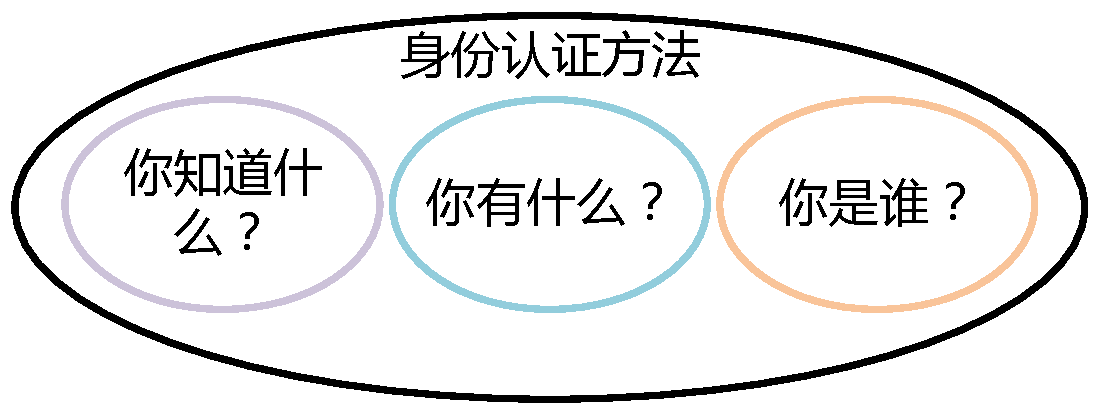
\includegraphics[width=0.5\textwidth]{figure/identification-method.pdf}
  \bicaption
    {身份认证方式}
    {Identification methods}
  \label{fig:identification-method}
\end{figure}

\textbf{(1)根据用户知道的信息。(你知道什么?)}日常生活中,最常用的是密码登录,这是一种依赖用户知道什么来识别是否为授权用户的方法,但一旦用户的密码被泄露,恶意用户输入相同的密码也会被系统识别为授权用户。

\textbf{(2)根据用户拥有的东西来。(你有什么?)}你回家会使用钥匙开门,钥匙就是你所拥有的东西,比起用户知道的信息,此处则体现为用户拥有的物理实体。

\textbf{(3)根据用户独特的身体特征。(你是谁?)} 随着智能手机技术进步和普及,目前人脸和指纹识别已经被用于手机系统登录和移动支付。人脸~\cite{12717}、指纹~\cite{Andrew2005Handbook}、虹膜~\cite{Wildes1997Iris}等是人体的固有特征,在随着时间变化上呈稳定状态,这样的认证方式比密码认证更加安全。 除此之外,个人独特的行为特征也可以被用于身份认证,比如:唇语识别~\cite{Cetingul2006Discriminative}、手写签名识别~\cite{Plamondona1989Automatic}、语音识别~\cite{Rashid2008Security}、步态识别~\cite{Boulgouris2005Gait}等。 


手写签名作为个体的一种重要的行为特征,在金融、法律、政府等领域广泛应用于用户身份的识别。 然而,这种认证方式也会受到恶意用户的攻击,举个例子,攻击者可以仿造存款用户的签名在一张取款支票上签名去银行取款,会造成实际用户的财产损失,降低银行存款安全性,大则可引发金融灾难。 而在政府或军事领域,仿造签名会造成更加难以想象的结果和混乱。 因此,在这些使用签名进行授权的领域,签名的识别变得尤其重要。在很久以前甚至现在,签名的识别主要依靠人工进行,签名验证者根据用户的历史签名来判断当前的签名是否为真实签名。这种方式,需要耗费昂贵的人力资源,且依赖于签名认证员的个人能力,容易造成误判。

信息技术使签名认证的自动化成为可能,自动签名认证系统得到研究和应用。 自动签名认证系统根据捕捉签名的方式不同,可以被分为两大类:离线签名认证系统和在线签名认证系统~\cite{鄢晨丹基于统计模型的}。 离线签名认证系统依靠签名图像的静态数据进行签名的比较来识别,而在线签名认证系统则依靠用户书写过程中记录下的时间序列数据(如书写速度、笔的压力等)来进行比较和识别。由于外加的时间维度信息,通常在线签名认证系统的表现优于离线签名认证系统。



无论是人工的签名识别还是自动签名认证系统,签名的识别过程都符合图~\ref{fig:signature-verification-architecture}
\begin{figure}[!htp]
  \centering
  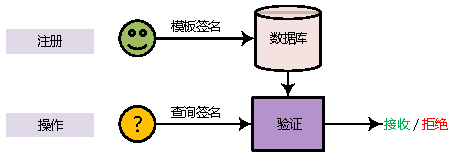
\includegraphics[width=0.7\textwidth]{figure/verification-work-flow.pdf}
  \bicaption
    {签名认证过程}
    {Signature verification architecture}
  \label{fig:signature-verification-architecture}
\end{figure}所示的签名认证过程。 在注册过程,用户需要输入多个他/她的签名存入数据库作为模板签名;在操作过程,用户签名作为查询签名提交给系统,系统将这个查询签名和模板签名进行比较,判断查询签名是否为真实签名。

一个签名认证系统的关键问题在于二方面:
\begin{enumerate*}[label=\itshape\alph*)\upshape]
    \item 需要能精准跟踪手写签名过程的行为信息。由于手写签名过程,笔记变化多样,而且运动幅度较小,对传感器的敏感度有较高要求。
    \item 用户体验和判别精度。用户体验体现在设备对用户的影响,比如是否需要特殊设备、是否需要用户佩戴设备等,还体现在模板签名数量。用户体验可能会和判别精度发生冲突,比如减少模板签名数量会导致判别精度下降,复杂的设备则能更细粒度跟踪签名运动轨迹,有利于判别精度的提升。
\end{enumerate*}

开展自动手写签名认证研究才能顺应用户对用户体验和安全提升上的诉求,将人力资源从签名识别中解放出来,提高签名识别的准确率和稳定性。目前国内外对手写签名认证的研究有很多基于开放数据集进行研究,存在一些问题,在普适性和用户体验上有待提高,探索签名的捕捉方式,可以降低签名认证的成本,让签名认证系统在现实中快速普及。

\section{国内外研究的现状与存在的问题}
这里从数据来源和手写签名认证建模两个方面,对近年来国内外学者在手写签名认证方面的研究进行分析。

(1) 数据来源

在数据来源方面,现有的手写签名认证系统的研究主要依赖于惯性传感器、手写平板设备和扫描图像,其中前二者可用于实现在线签名认证系统,而离线签名认证系统则依赖于扫描图像。

基于惯性传感器的方法~\cite{levy2018handwritten,griswold2019wearables,bunke2011online}利用穿戴在手上的惯性传感器 (如加速度计、陀螺仪等) 跟踪手部运动,提取个人签名时手部独特的运动特征。这种方法要求用户佩戴可穿戴设备(如定制设备、腕表和装有惯性传感器的笔等),会给用户造成额外的负担或困扰,而且设备穿戴的位置不宜固定,这会对签名认证的精度造成较大影响。{}

基于手写平板设备的方法~\cite{fischer2015robust,kholmatov2005identity,sae2013simple}利用手写笔或者手指在平板书写留下的动态轨迹来识别签名。这样的轨迹在静态轨迹基础上,还能获得书写时对平板压力和轨迹变化速度等时间序列数据,相比仅仅用静态图像的认证方式可以大大提高认证精度。但是这种认证方式需要一个手写平板,而且限制字迹只能写在平板而不是纸上,这是与日常生活中的书写场景是不同的。

基于扫描图像的方法~\cite{hafemann2017learning,hafemann2018fixed,ferrer2005offline,kalera2004offline}使用扫描仪扫描并切割出签名图像,直接比较存在数据库中的静态图像,与人工判别的方式在数据来源上有相似之处。由于没有书写过程的数据,这种仅仅比较写出结果的方法,往往无法判断出在字迹上看起来很相似的伪造签名。但这种签名认证方式的优势是具有通用性和较好的用户体验,不会给用户签名过程造成干扰,用户可以依照平时的签名习惯来签名。

(2) 手写签名认证建模

手写签名认证建模方面的方法有多种,离线和在线签名认证系统需要采取不同的建模方法。

离线签名认证系统通常采用图像匹配的方法~\cite{赵桂敏2003手写签名的快速认证},比如人工神经网络(Artificial Neural Network, ANN)~\cite{chandra2016offline}、像素匹配 (Pixel Matching Technique, PMT)~\cite{bhattacharya2013offline}等。 

在线签名认证系统~\cite{李成华基于1}采用的方法可以分为两类:\textit{a)} 基于函数的方法,使用长短时记忆网络 (Long Short-Term Memory, LSTM)~\cite{hochreiter1997long}、隐马尔科夫模型 (Hidden Markov Model, HMM)~\cite{rabiner1986introduction,雷涛隐马尔可夫模型下视频手写签名认证算法研究}、 动态时间规整 (Dynamic Time Warping, DTW)~\cite{鄢晨丹基于统计模型的}等这些函数型方法直接在时间序列上进行处理并识别;\textit{b)}基于特征的方法,这种方法将时间序列从时域数据转化为频域数据,可以用到的变换方法有离散傅里叶变换 (Discrete Fourier Transform, DFT)、离散余弦变换 (Discrete Cosine Transform, DCT)~\cite{李成华基于}等,进而通过频域特征上进行特征选择实现数据降维,再利用提取到的特征进行比较或者分类。匹配方法也可以使用DTW或者欧式距离,而分类方法可以使用一些机器学习方法,比如支持向量机 (Support Vector Machine, SVM)、随机森林 (Random Forest)、朴素贝叶斯 (Naive Bayes)等~\cite{周志华2016机器学习}。这些方法一般是在公开数据集上进行实现和评估,当有新数据源时,需要设计新的合适的模型。而且,由于使用的是公开数据集,这些研究很少评估系统的鲁棒性,比如不同时间段对签名的影响。

\section{本文研究内容与创新点}
\subsection{研究内容与所做的工作}
针对现有存在研究的主要问题,本文研究设计一种非侵入式的,具有鲁棒性、安全性、低时延的在线手写签名认证方案,主要的研究内容和所做的工作如下:

(1) 手写签名认证数据源的研究

本文提出利用声波感知技术来跟踪手写签名时的手部运动和笔的运动状态,进而推断是否为本人签名。声波对不是陌生的信号,人们用声带发射声波,用耳膜接收声波,以此来实现对这个世界的感知。本文采用声波相位相关信息,利用计算弦的方法避开了求相位时去直流的问题,实现了微小动作的跟踪。


(2) 手写签名认证模型的研究

针对声波相位相关信息设计了合适的特征提取和用户独立的识别模型。手写签名动作所产生的影响在相位信号中体现为低频信号,而高频信号则是由环境或者硬件造成的噪声所产生,因此通过将时域数据转换到频域数据,然后提取低频系数的方法,将手写签名动作的信息提取出来。当判别一个查询签名是否为真的时候,需要比较查询签名的特征与模板签名特征的之间的相似度,本文对多个模板签名的特征进行融合操作,获得几个固定数目的特征矩阵,查询签名的特征矩阵和这些矩阵作差获得相似矩阵。最后采用比传统分类器有更好表现的深度神经网络 (Deep Neural Network, DNN)\cite{Schmidhuber2015Deep} 作为二分类器来分类相似矩阵。

(3) 性能评估分析和原型系统实现

对该方案进行了全面的评估,包括验证精度、交叉用户可用性、硬件补偿的效果、系统鲁棒性、微基准实
验、对比实验和重放攻击等。准确性测试以 AUC (Area Under Curve) 和 EER (Equal Error Rate) 作为度量指标;在鲁棒性测试中,改变环境、距离、日期等来对系统进行测试;在安全性测试中,测试系统对重放攻击的抵抗能力;在微基准测试中,改变一些超参数观察系统的变化;在性能测试中,通过度量系统时延。利用三星Galaxy S6智能手机设计并实现基于声波的手写签名认证原型系统,对其运行效率进行了评估。


\subsection{研究创新点}

本文主要有如下两个方面的创新点:

(1)第一次提出使用声波感知技术来实现一个在线签名认证,并基于主流智能手机实现了一个非侵入式、用户友好、安全、低延迟、准确的在线签名认证系统。相比于之前的声波感知技术研究,在避免去直流的前提下提取到了相位相关信息,用以跟踪手写签名时所产生的微小的动作。

(2)使用DCT提取信号中低频部分作为手写签名行为的特征,使用深度学习进行分类,相比传统的分类方法获得了更好的表现。

\section{论文结构}

本文共分五章,每章的内容安排如下:

第一章为绪论,主要阐述了手写签名认证研究的背景和研究意义、国内外相关技术研究现状、本文的研究内容以及主要的创新点。

第二章是手写签名认证相关技术的分析,首先分别从手写签名认证中的感知技术和手写签名认证中的建模方法两个方面对现有的研究进行了综述,然后分析总结了现有研究存在的问题。基于存在的问题,提出了本文的技术路线,最后介绍了本文涉及到的相关理论和技术。

第三章是基于声波的手写签名认证的关键技术研究,首先对要解决的问题进行了描述,然后提出一种包含四个模块的基于声波的手写签名认证方案,然后对声波相位相关信号感知技术、特征提取技术、相似性度量技术和深度学习模型等关键技术进行了深入研究,详细介绍了方案中各模块的设计思想和技术细节。

第四章对基于声波的手写签名认证方案进行了实验验证,首先描述了实验方法和采集的数据集,提出验证指标和用于对比的方案,之后实验验证本文方案的识别性能,最后探究影响识别性能的主要因素。

第五章实现了一个基于安卓智能手机的手写签名认证系统,首先对系统的用户需求进行分析,然后完成系统架构的设计,最后评估系统的性能效果。

第六章是总结和展望,对本文的研究内容进行了总结,对未来的工作进行了展望。

\chapter{手写签名认证相关技术分析}
\label{chap:related-work}
目前手写签名认证的任务呈现普适性、便利性、模型用户无关的发展趋势,对实施技术的要求越来越高,本章首先介绍手写签名认证研究综述,分析总结现有研究存在的问题,然后针对存在的问题提出本文的技术路线,最后对本文涉及到的相关理论与技术进行介绍。
\section{手写签名认证研究综述}
手写签名认证研究所涉及到的技术领域比较广泛,如传感器技术、图像技术、通信技术、机器学习等等。应用这些技术需要解决的最核心问题主要有两点,即“签名行为的数据怎么采集”和“采集到的数据怎么处理”,本文从这两方面对现有研究进行综述。
\subsection{手写签名认证中的感知技术}
(1) 基于扫描图像的手写签名认证

从图像上签名通常可以分为三类~\cite{Hanmandlu2005Off}:简单的、草书的、图形的签名,如表~\ref{tab:signatures-images}所示。
\begin{table}[!hpb]
  \centering
  \bicaption
    {真实签名与仿造签名图像~\cite{Hanmandlu2005Off}}
    {Genuine and forged signatures}
  \label{tab:signatures-images}
  \begin{tabular}{|c|m{0.2\textwidth}|m{0.2\textwidth}|m{0.2\textwidth}|} \toprule 
    类型 & 真实签名 & 熟练仿造签名 & 不熟练仿造签名\\ \midrule
   简单& 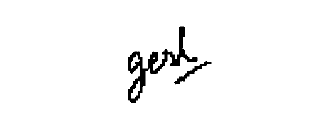
\includegraphics[width=0.2\textwidth]{figure/signature-1.png}&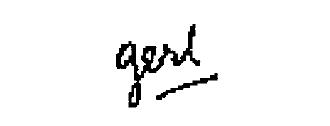
\includegraphics[width=0.2\textwidth]{figure/signature-2.png}&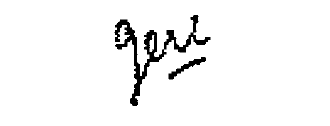
\includegraphics[width=0.2\textwidth]{figure/signature-3.png} \\ \midrule
    草书&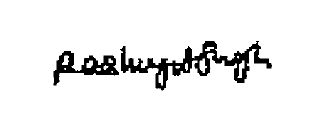
\includegraphics[width=0.2\textwidth]{figure/signature-4.png}&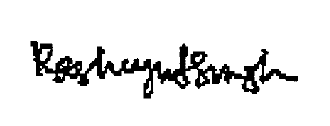
\includegraphics[width=0.2\textwidth]{figure/signature-5.png}&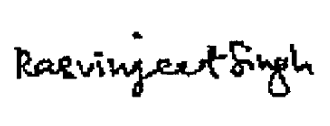
\includegraphics[width=0.2\textwidth]{figure/signature-6.png} \\ \midrule
    图形&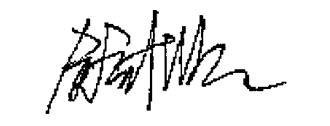
\includegraphics[width=0.2\textwidth]{figure/signature-7.png}&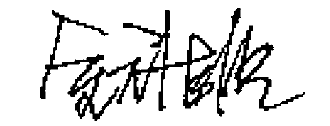
\includegraphics[width=0.2\textwidth]{figure/signature-8.png}&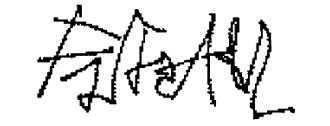
\includegraphics[width=0.2\textwidth]{figure/signature-9.png} \\ 
        \bottomrule
  \end{tabular}
\end{table}
简单的签名便是平时的普通签名;草书签名是写的过程有比划连在一起的签名;图形的签名则是用草书方式描述几何模式的签名。从图像上看真实签名、熟练仿造签名、不熟练仿造签名之间有很大相似之处,但是细看不同之处也有很多,离线签名认证利用这些从纸上扫描出来的图像进行识别。

Madasu~\cite{Hanmandlu2005Off}等让签名者使用黑笔在白纸上签名,之后使用扫描仪以200 dpi的分辨率扫描获得图像,并经过50\%的重采样将像素点数量减少到原来的一半,40名志愿者参与数据集构建,每名志愿者提供15个真实签名和15个仿造签名,总共1200个签名图像。Subhash~\cite{chandra2016offline}等人邀请了18名志愿者,每名志愿者提供15个真实签名和15个仿造签名,总共540个尺寸为$850\times360px$的签名图像。除了自己手机签名数据集外,目前公开的签名图像数据集有:MCYT\footnote{http://atvs.ii.uam.es/atvs/mcyt75so.html}、CEDAR\footnote{https://cedar.buffalo.edu/Databases/CDROM1/}、Brazilian PUC-PR~\cite{freitas2008brazilian}。 签名的公开数据库文字上以英文居多,Brazilian PUC-PR则提供巴西葡萄牙语的签名数据。采集签名的最传统方式是直接让志愿者写在纸上,然后扫描,这种方式耗费人力。而最近,可以让签名者将签名写在平板上,仅仅使用静态轨迹数据就可以作为离线签名的数据集,同时兼顾离线签名认证研究和在线签名认证研究对数据集的需求。

(2) 基于惯性传感器的手写签名认证
  
在手写签名的过程中,签名者通过手和笔的运动来留下签名字迹,运动过程中手和笔的运动加速度和方向会发生变化,因此可以通过给手或者笔配备惯性传感器(可以将惯性传感器佩戴在手上,如智能腕表,也可以将惯性传感器装在笔上)实现对此运动过程的记录。常见的惯性传感器包括加速度计和陀螺仪,这两个惯性传感器均可产生三维的时间序列数据,分别记录物体线性加速度和角运动,用于描述物体在三维空间中的运动状态。

Alona~\cite{Levy2018Handwritten}等人提出一种可穿戴的手写签名认证系统如图~\ref{fig:smartwatch-inertial-sensor}所示,
它使用一个戴在签名手上的智能腕表上的惯性传感器和加速度计实现对签名动作的记录,虽然腕表目前的普及率还远不如智能手机,但腕表逐渐被大众所接受,所以这种方法还是具有普适性的。Isaac\cite{8698222}等人使用腕表实现了在多个场景下的手写身份识别,并对多种不同强度的攻击方式进行评估。Bunke~\cite{Bunke2015Online}等人在普通笔的笔尖附近贴上了一个带线的加速度计,使用如图~\ref{fig:pen-inertial-sensor}所示,通过细带电缆将加速度时间序列传输到电脑端,据此分析签名动作。
\begin{figure}[!htp]
  \centering
  \begin{minipage}[t]{0.22\textwidth}
    \centering
    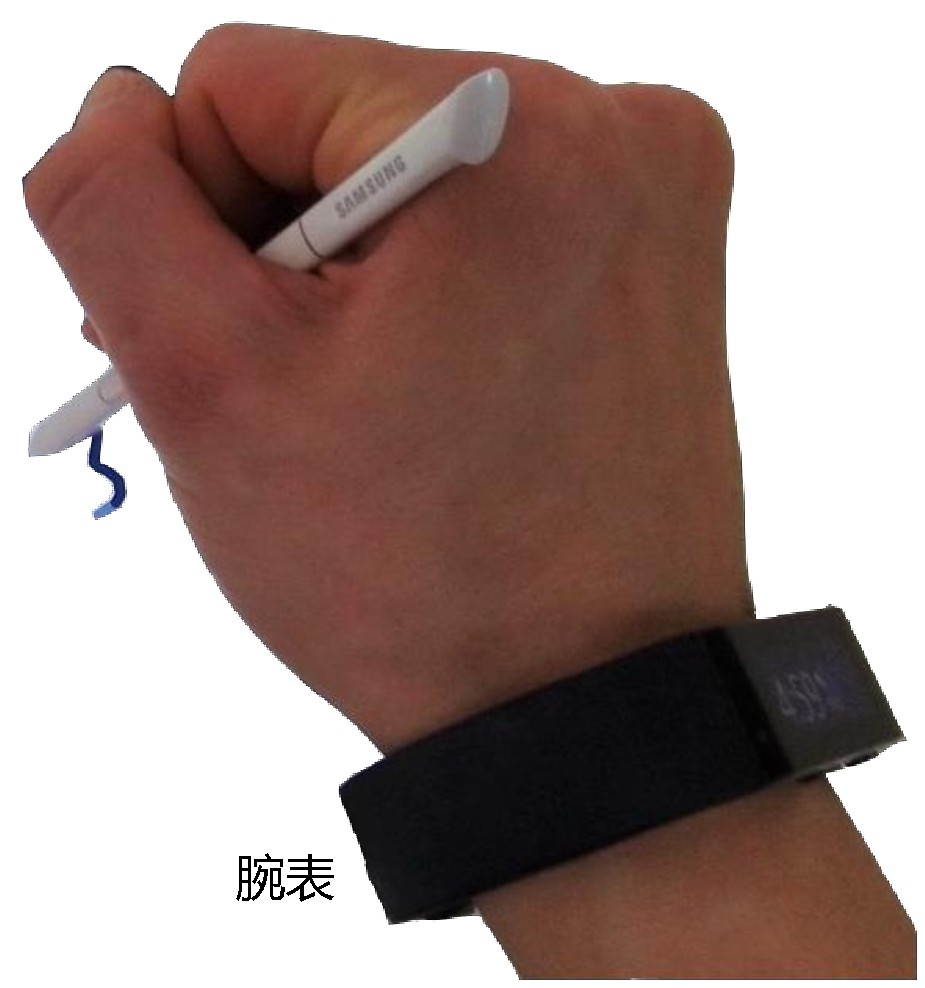
\includegraphics[width=\textwidth]{figure/smartwatch.pdf}
      \bicaption{用腕表上惯性传感器}
      {Using inertial sensors on swatches}
        \label{fig:smartwatch-inertial-sensor}
  \end{minipage}
  \centering
  \begin{minipage}[t]{0.49\textwidth}
    \centering
    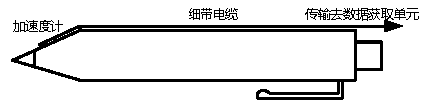
\includegraphics[width=\textwidth]{figure/acceleration-pen.pdf}
    \bicaption
    {用笔上的惯性传感器}
    {Using inertial sensors on pens}
    \label{fig:pen-inertial-sensor}
   \end{minipage}
\end{figure}

(3) 基于手写平板设备的手写签名认证


如图~\ref{fig:signing-tablet}所示,
\begin{figure}[!htp]
  \centering
  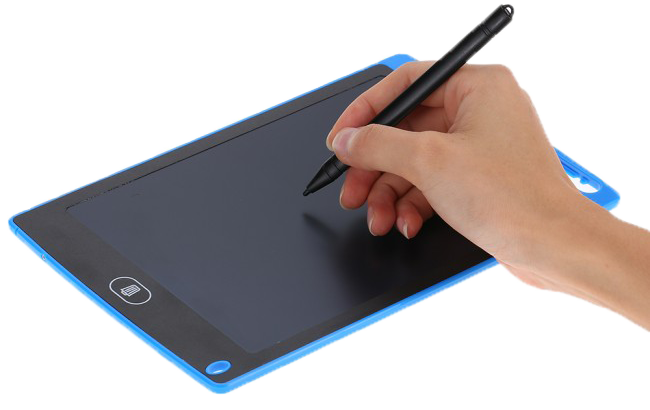
\includegraphics[width=0.3\textwidth]{figure/tablet.png}
  \bicaption
    {在平板上签名}
    {Signing on a tablet}
  \label{fig:signing-tablet}
\end{figure}
签名使用手写笔在平板上签名,由平板记录签名轨迹,手写屏除了能记录轨迹还能记录压力值,如果使用智能笔则还能记录笔的倾斜角,因此采集到的时间序列数据可以包括:采样点的二维坐标、笔尖压力值、笔的水平偏角和垂直偏角~\cite{房育勋在线签名认证若干关键问题研究}。Alona~\cite{Levy2018Handwritten}等人在用腕表上惯性传感器跟踪签名动作的同时,记录签名轨迹,轨迹数据除了可以给仿造者提供仿造学习材料,还可以用于和两个经典系统~\cite{fischer2015robust,kholmatov2005identity}做对比实验。

目前,可用于在线签名认证研究的公开数据集有:MCYT-100\footnote{http://atvs.ii.uam.es/atvs/mcyt100s.html}、SUSIG~\cite{kholmatov2006sigsa}、SVC2004~\cite{10.1007/978-3-540-25948-0_3}、SCUT-MMSIG~\cite{10.1007/978-3-319-69923-3_78}等。

MCYT-100是MCYT数据库的一个子集,包含100个签名者的数据,每个签名者有25个真实签名和25个仿造签名,总共5000个签名样本。至于SUSIG数据库,Kholmatov~\cite{kholmatov2006sigsa}等人使用一个分辨率为300 dpi、具有128层垂直压力感知、100 Hz采样率的压力感知触摸平板,邀请110位志愿者参与真实签名的收集,其中包括年龄在21岁到52岁之间的29位女性和81位男性,每位志愿者分两个时间段提供20个真实签名,而仿造签名由仿造者观看签名过程并练习后为每个真实签名者提供5个仿造签名,实验结果证明签名是一个复杂度取决于签名者生物特征。SV2004是2004年香港科技大学举办在线认证比赛提供的数据库,针对比赛中的两个任务,该数据库提供两个数据集,每个数据集都包含100个签名集合,每个签名集合包含20真实签名和20熟练仿造签名,不同的是其中一个数据集只包含坐标时间序列,而另外数据集则还包含笔的方向和压力,两个数据集中前40个签名集合完全不同,而后60个集合仅仅是笔的方向和压力不同。比赛中,成绩最好的第一个任务EER=2.84\%,第二个任务EER=2.89\%。

SVC2004包含中文签名和英文签名,SCUT-MMSIG则是由华南理工大学采集的纯中文签名,所以如果做针对中文签名认证研究的研究者可以考虑这两个签名数据作为评估数据集。

本领域的研究者基于公开数据集做了很多工作。Kholmatov~\cite{kholmatov2005identity}赢得SVC2004的冠军。2015年,Fischer~\cite{fischer2015robust}在两个数据集上进行了评估,在MCYT数据集上使用5个模板签名时在随机仿造(random forger)和熟练仿造(skilled forger)情况下的EER分别为1.06\%和3.94\%,在SUSIG数据集使用5个模板签名时在随机仿造和熟练仿造情况下的EER分别为1.34\%和3.09\%。

\subsection{手写签名认证中的建模方法}

已经有一些文章对签名认证研究进行了综述,如上世纪80年代Rejean~\cite{plamondon1989automatic}等人的综述,那时研究者开始用人工神经网络实现签名认证,90年代的Franck~\cite{leclerc1994automatic}和2000年代的Donato等人~\cite{impedovo2008automatic}的综述,在2012年Donate等人对之前的综述进行了补充~\cite{impedovo2012handwritten}。近年来,Luiz G.~\cite{hafemann2017offline}等人对离线签名认证进行了综述,并加入基于深度学习的相关研究内容,Prathiba~\cite{prathiba2014online}等人对在线签名认证进行了综述。

Kai~\cite{huang1997off}提取了签名图像的多种粒度的局部对比几何特征,为每种粒度的特征使用一个适配的多层感知机,多个感知机的输出作为一个决策感知机的输入,决策感知机用于输出最后二分类的结果,在一个超过3000个样本的数据集中达到90\%的分类准确率。

为所有用户训练的模型称为写者独立模型(writer-independent model, WI model),需要为每个用户训练一个的模型称为写者依赖模型(writer-dependent model, WD model)。有些系统会使用熟练仿造签名进行用户独立模型的训练~\cite{rivard2013multi,eskander2013hybrid},有些系统使用熟练仿造签名进行用户独立模型训练~\cite{yilmaz2016score,rantzsch2016signature,hafemann2017learning}后会再用另外一个不同的数据集进行测试。有些系统混合使用用户独立模型和用户依赖模型,使用用户独立模型用于特征提取,利用提取到的特征为每个用户训练一个小型的用户依赖模型,综合了两种模型的优点。随着深度学习在图像领域的广泛应用,现在可以用DNN直接从图像中学习得到特征。Hafemann~\cite{hafemann2016writer}使用一个卷积神经网络(Convolutional Neural Network, CNN)作为特征提取器,再用SVM为每个用户训练一个用户依赖模型,之后进一步提出了多任务的卷积神经网络框架~\cite{hafemann2017learning},可同时提取到区分签名真实性和用户间差异的特征。

来自签名的动态特征提供了某个时间的笔画数目和顺序、速度、笔的压力等相关信息,可以使签名唯一性得到更好的保障。 Alisher~\cite{kholmatov2005identity}的在线签名认证系统将签名的识别视为一个二分类的模式识别问题,DTW被用于建立给定签名的合法性:给定一个签名与被申明用户的参考签名计算DTW距离,计算出与最近、最远、模板参考签名的DTW距离,生成3维的特征向量用于后续的分类,在使用熟练仿造者的测试中,EER达到2.8\%。S.A. Daramolo~\cite{daramola2010efficient}为了建立签名的特征序列之间的一致关系,将DTW用于训练和分类。Alona~\cite{levy2018handwritten}等人结合使用DCT和DTW,得到一个特征向量,最后输入到一个用户独立的二分类器进行判别。

HMM被证明可以有效用于签名认证,因为它可以高度适应个体间差异,Mohammad M. Shafli 和 Hamid R. Rabiee~\cite{shafiei2003new}介绍了使用变长分段和HMM实现的在线签名认证系统,实现了错误接受率(False Accept Rate, FAR)和错误拒绝率(False Reject Rate)分别为4\%和12\%的性能。

Syed Khaleel Ahmed~\cite{ahmed2009automatic}等人设计的签名认证系统由4个模块组成,分别是特征提取模块、参考模块、样本模块、智能决策模块:特征提取模块用于捕捉二维坐标和笔的压力的时间序列;参考模块用于存储训练数据;样本模块包含用于验证的数据;智能决策模块则是一个自组织映射神经网络,用于对数据进行聚类,将高维数据映射为一维或二维数据。%Alona~\cite{levy2018handwritten}等人使用DCT对惯性传感器的数据转换去前几位低频系数,减少了数据量,将查询签名的DCT系数和模板签名的低频系数求DTW距离并去最小值,得到一个特征向量,最后输入到一个用户独立的二分类进行判别。

\section{现有研究存在的问题}
根据上文对于手写签名认证的研究综述,对现有研究存在的问题进行分析总结。

(1) 手写签名认证的感知技术中存在的问题

目前,手写签名认证中通常采用的感知技术方案主要有三种:基于惯性传感器、基于扫描图像、基于手写平板设备的解决方案。基于惯性传感器的主要问题是需要在用户或者笔上佩戴惯性传感器:如果是笔上安装惯性传感器,则要求定制的笔,不便于推广;如果是要求用户佩戴腕表之类的设备,则该设备必须在用户写字的手上,在可穿戴设备还没大量普及的前提下该要求过于苛刻,而且腕表在手上的位置变化也会影响到判别的错误率。基于扫描图像的方法,比较符合用户的习惯,但是由于动态特征的缺失,熟练的仿造者可以花足够的时间去仿造签名以达到在静态形状上尽可能像,这给离线签名认证系统带来了巨大挑战。基于手写平板设备的方法,需要手写平板,如果用手指写则不符合用户平时的签名习惯,如果也是用笔在平板上写并且给予书写轨迹的反馈,由于需要特殊的设备而提高了普及化的难度。

(2) 手写签名认证建模技术中存在的问题

DTW是一种非常经典用于计算两个不同长度序列之间距离的算法,其在模式识别中的应用十分广泛。然而,DTW技术具有两个明显的缺点:1)计算开销大;2)对仿造签名进行规整使得验证更加困难。

而HMM模型是无记忆性的,它的当前状态只与其前一个状态有关,无法利用更多复杂信息。

使用深度学习进行用户无关的模型训练会引发巨大的训练开销,而且越是复杂的网络要求有足够大的数据集防止其过拟合。目前的系统大多在公开数据集进行测试,过于追求精度的提升,很少有度量在识别时间上的开销,因此复杂的方法在现实中不一定可行。

\section{本文的技术路线}

本文针对目前手写签名认证中的感知技术和手写签名认证中的建模方法的研究中存在的问题,提出了本文的技术路线,如图~\ref{fig:technology-roadmap}所示,主要是具有递进关系的四种技术研究,下面将分别介绍这四种技术。
\begin{figure}[!htp]
  \centering
  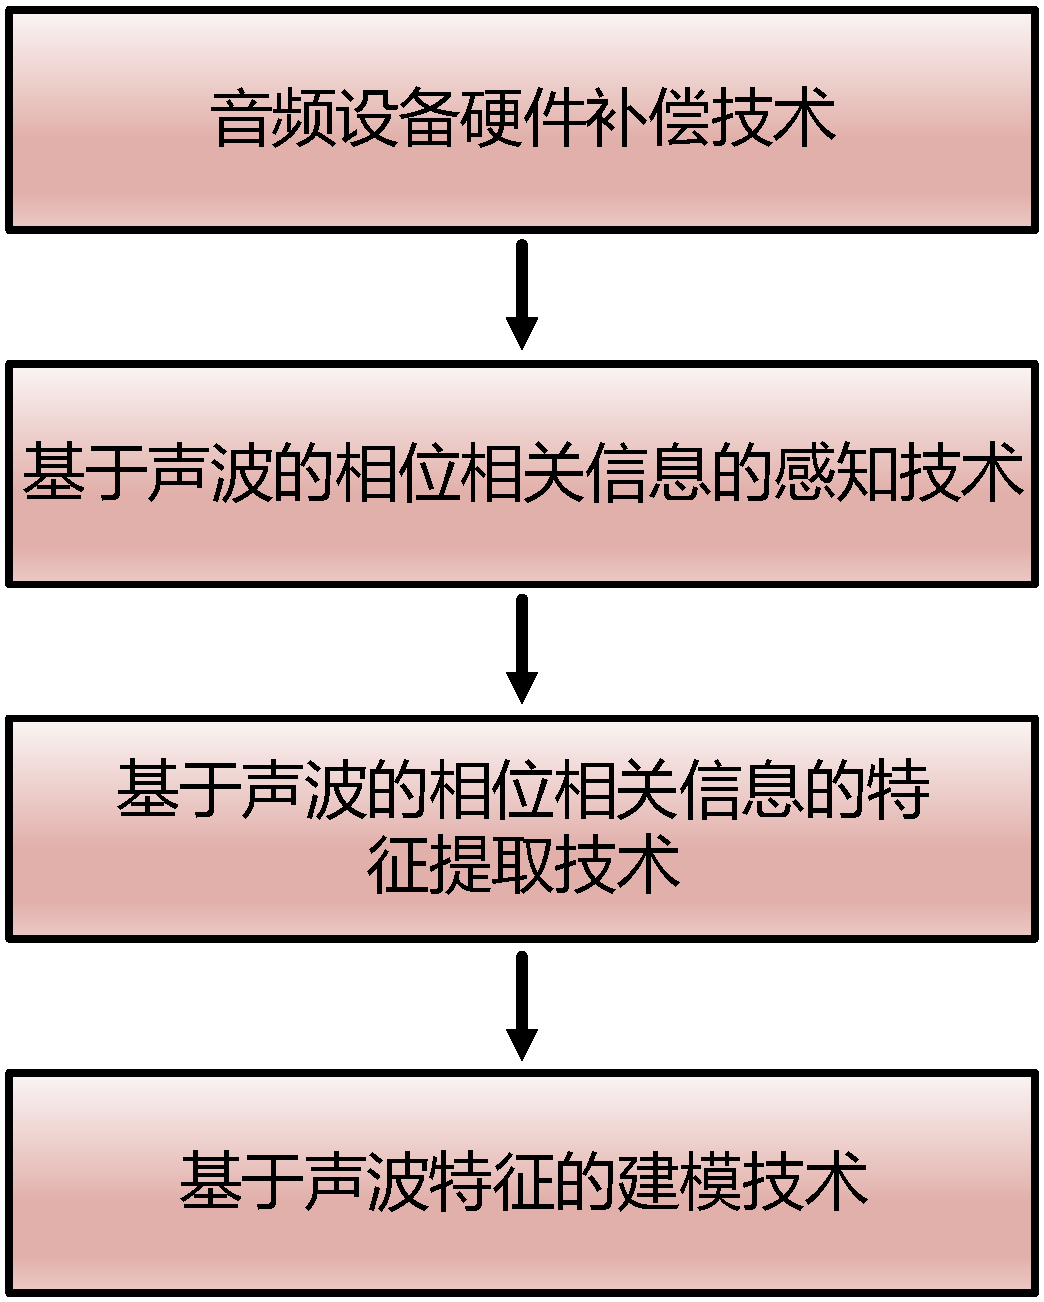
\includegraphics[width=0.3\textwidth]{figure/technique-road.pdf}
  \bicaption
    {本文的技术路线}
    {The technology roadmap}
  \label{fig:technology-roadmap}
\end{figure}

(1) 音频设备硬件补偿技术

本文的数据采集和原型系统实现是基于智能手机上的音频设备。然而,智能手机上的音频设备主要用于娱乐、通信等,其主要设计用途并不包括声波感知,因此当利用智能手机发送高频的声波信号(17 kHz以上),尤其是同时发送多个高频声波信号时,每个频率上声波实际发送能量差异可能会很大。本文针对智能手机上音频设备的硬件不足,进行了硬件补偿,以便目标频率声波的发射能量不至于太小。

(2) 基于声波的相位相关信息的感知技术

从麦克风设备中获得的是一个原始的音频数据,其中包括了人交谈的声音、环境噪音等人耳可听见和不可听见的声音。这些声波信号并不是本文所需要的,需要对原始的接收信号进行转换以获得两个经降采样的正交信号,这两个正交信号可用于计算相位。相位信息与声波的传播路径长度直接相关,环境中一些周期性运动例如笔记本散热器叶片的转动也会对相位信息产生影响,因此需要对两个正交信号进行去噪,然后提取相位相关的信息。

(3) 基于声波的相位相关信息的特征提取技术

声波的相位信息和声波传播路径直接相关,签名时手的运动引起声波传播路径长度的变化,从而导致相位的波动,而手的运动对相位的影响呈现为低频信号,高频信号则为噪声。本文使用DCT将相位相关信号从时域转换到频域,取低频系数作为特征提取和选择的结果。

(4) 基于声波特征的建模技术

本文认为签名真实性的判别是个二分类问题。对一个用户,在收集模板签名之后,根据所有模板签名的特征矩阵,计算出三个用于和查询签名比较的矩阵(最小值、最大值、平均值),和查询签名的特征矩阵通过做差得出距离矩阵。本文设计一个多层CNN模型,以距离矩阵作为输入进行二分类。

\section{相关理论与技术简介}

\subsection{智能手机音频设备的位置和配置}

三星Galaxy S6是三星公司在2015年5月推出的一款智能手机,是本文原型系统ASSV使用的智能手机,如图~\ref{fig:audio-device-smartphone}所示。
\begin{figure}[!htp]
  \centering
  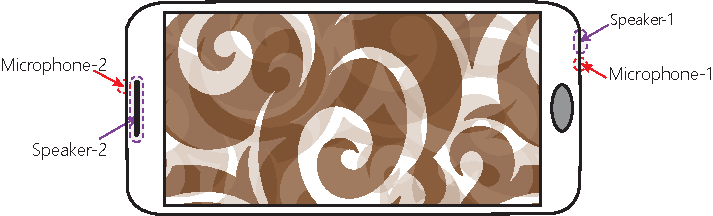
\includegraphics[width=0.5\textwidth]{figure/smartphone.pdf}
  \bicaption
    {智能手机上的音频设备}
    {Audio devices on smartphones}
  \label{fig:audio-device-smartphone}
\end{figure}
该智能手机搭载了2个扬声器和2个麦克风:
\begin{enumerate*}[label=\alph*)]
    \item 一个降噪麦克风(Microphone-2)位于机身的上壁,对高频信号较为敏感,且原来用户打电话时的发生点,可以用于记录背景噪声;
    \item 一个主麦克风(Microphone-1)位于机身的下壁,对人声比较敏感(通常低于8 kHz),用于记录通话语音;
    \item 一个通话扬声器(Speaker-2)位于屏幕上部,用于通话时对准耳朵;
    \item 一个主扬声器(Speaker-1)位于机身的下壁,位于主麦克风的旁边。
\end{enumerate*}

\begin{table}[!hpb]
  \centering
  \bicaption{三星Galaxy S6的硬件配置}{Hardware settings of Samsung Galaxy S6}
  \label{tab:smartphone-hardware-setting}
  \resizebox{\textwidth}{!}{
\begin{tabular}{|l|l|l|}
\hline
\multirow{2}{*}{Body}     & Dimensions  & 143.4 x 70.5 x 6.8 mm (5.65 x 2.78 x 0.27 in)                          \\ \cline{2-3} 
                          & Weight      & 138 g (4.87 oz)                                                                            \\ \hline
\multirow{4}{*}{Platform} & OS          & Android 5.0.2 (Lollipop), upgradable to Android 8.0 (Oreo); TouchWiz UI \\ \cline{2-3} 
                          & Chipset     & Exynos 7420 Octa (14 nm)                                                \\ \cline{2-3} 
                          & CPU         & Octa-core (4x2.1 GHz Cortex-A57 \& 4x1.5 GHz Cortex-A53)                \\ \cline{2-3} 
                          & GPU         & Mali-T760MP8                                                            \\ \hline
\multirow{2}{*}{MEMORY}   & Card slot   & No                                                                      \\ \cline{2-3} 
                          & Internal    & 32/64/128 GB, 3 GB RAM                                                  \\ \hline
\multirow{4}{*}{Sound}    & Loudspeaker & Yes                                                                     \\ \cline{2-3} 
                          & 3.5mm jack  & Yes                                                                     \\ \cline{2-3} 
                          &             & 24-bit/192kHz audio                                                     \\ \cline{2-3} 
                          &             & Active noise cancellation with dedicated mic                            \\ \hline
\multirow{5}{*}{Battery}  &             & Non-removable Li-Ion 2550 mAh battery                                   \\ \cline{2-3} 
                          & Charging    & Fast battery charging 15W                                               \\ \cline{2-3} 
                          &             & Qi/PMA wireless charging (market dependent)                             \\ \cline{2-3} 
                          & Talk Time   & Up to 17 h (3G)                                                         \\ \cline{2-3} 
                          & Music play  & Up to 49 h                                                              \\ \hline
\end{tabular}
}
\end{table}
该型号智能手机的硬件配置如表~\ref{tab:smartphone-hardware-setting}~\footnote{https://www.gsmarena.com/samsung\_galaxy\_s6-6849.php}所示,其具有较好的计算性能和较大的内存空间,支持24-bit/192kHz的音频设备,可以满足本研究对设备的要求。

\subsection{声波信号下转化}
将智能手机上麦克风的采样率设置为48 kHz,由于接收和发射声波的设备在同一智能手机共享一个时钟频率,因此接收端和发送端之间不存在载频偏移(Carrier Frequency Offset, CFO)。因此,可使用图~\ref{fig:sound-signal-down-conversion}
\begin{figure}[!htp]
  \centering
  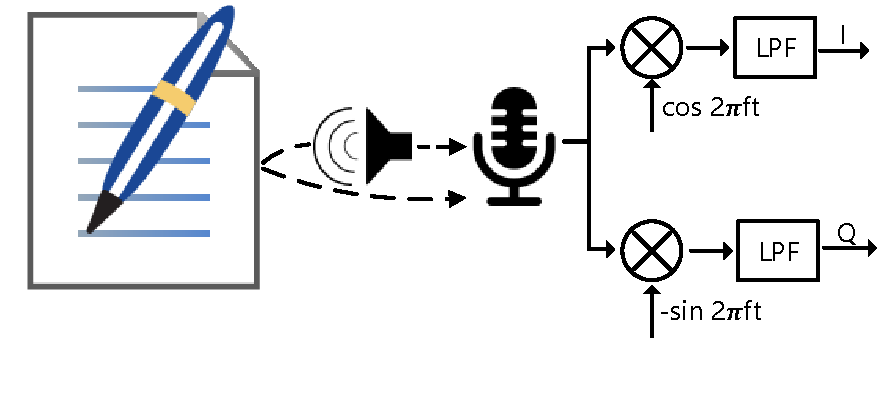
\includegraphics[width=0.5\textwidth]{figure/down-conversion.pdf}
  \bicaption
    {声波信号下转化}
    {Sound signal down conversion}
  \label{fig:sound-signal-down-conversion}
\end{figure}
所示的相干解调器结构将接收到的声波信号下转化为基带信号~\cite{tse2005fundamentals},接收信号被分成两份副本,分别乘以发射信号$-cos2\pi ft$和它的相位偏移信号$-sin2\pi ft$,再经过一个低通滤波器获得同相(In-phase)和正交(Quadrature)分量。

LLAP~\cite{wang2016device}中对信号下转化的过程进行了解释。为了更好地理解数字下转化过程,假设一个信号路径$p$的路径长度随时间变化的函数为$d_p\left( t\right)$。来自路径$p$的信号可以表示为:
\begin{equation}
  R_{p}\left( t\right) = 2A^{'}_{p}cos \left( 2\pi ft - 2\pi fd_{p}\left( t \right) / c - \theta_{p} \right).
\end{equation}
其中,$2A^{'}_{p}$是接收信号的强度,$2\pi fd_{p}\left( t \right)/c$是产生于传播延迟$\tau=d_{p}\left(t\right)/c$的相位间隔,$c$是声音传播速度。初始相位$\theta_p$是硬件延迟和由于反射而发生相位反转的结果。按照图~\ref{fig:sound-signal-down-conversion}中的结构,将接收信号乘以$cos\left( 2\pi ft \right)$,得到:
\begin{equation}
\begin{aligned}
&2A_{p}^{'}cos \left( 2\pi ft - 2\pi fd_{p}\left( t\right)/c - \theta_{p} \right) \times cos\left( 2\pi ft\right) \\ 
= \quad &A_{p}^{'}\left( cos\left( -2\pi fd_{p}\left( t\right)/c - \theta_{p} \right) + cos\left( 4\pi ft - 2\pi fd_{p}\left( t\right)/c - \theta_{p} \right)  \right).
\end{aligned}
\end{equation}
第二个子项的频率为$2f$,属于高频,可以被低通滤波器去除。所以可以获得基带信号的同相分量(I-component)为:
\begin{equation}
 I_{p}\left( t\right) = A_{p}^{'}cos \left( -2\pi fd_{p}\left( t\right)/c - \theta_{p} \right).
\end{equation}
相似地,可以获得正交分量(Q-component)为:
\begin{equation}
Q_{p}\left( t\right)=A_{p}^{'}sin\left( -2\pi fd_{p}\left(t \right)/c - \theta_{p} \right).
\end{equation}
结合这两个分量,分别作为复数的实部和虚部,可以得到复数形式的基带信号($j^2=-1$):
\begin{equation}
B_{p}\left( t\right) = A_{p}^{'}e^{-j\left( 2\pi fd_{p}\left( t\right)/c + \theta_{p} \right)}.
\end{equation}
因此,在路径$p$上的相位为:
\begin{equation}
\phi_{p}\left( t\right) = -\left( 2\pi fd_{p}\left( t\right)/c + \theta_{p} \right).
\end{equation}
当$d_{p}\left(t\right)$变化一个声波波长的长度$\lambda = c/f$时,相位$\phi_{p}\left( t\right)$变化$2\pi$。
\subsection{离散余弦变换}
\label{sec:dct}
正交变换和逆变换在维纳滤波器中充当重要角色,DCT~\cite{ahmed1974discrete}是一种正交变换,可以用于实现一个维纳滤波器和模式识别中的特征选择。在模式识别中DCT可以用于特征选择,对原始数据进行降维,以便于进行分类。一个序列$X(m),m=0,1,\cdots,(M-1)$的DCT可以为定义为:
\begin{equation}
\label{equ:dct}
\begin{aligned}
G_{x}\left( 0\right) &= \frac{\sqrt{2}}{M} \sum_{m=0}^{M-1}X\left( m\right), \\
G_{x}\left( k\right) &= \frac{2}{M} \sum_{m=0}^{M-1}X\left( m\right)cos\frac{\left(2m+1\right)k\pi}{2M}, k=1,2,\cdots,(M-1).
\end{aligned}
\end{equation}
$G_{x}(k)$是第k个DCT系数。值得注意的是,基向量集合$\{ 1/\sqrt{2}, cos((2m+1)k\pi)/(2M) \}$实际上是一组离线切比雪夫多项式。
DCT的逆变换(Inverse Discrete Consine Transform, IDCT)可以被定义为:
\begin{equation}
\label{equ:idct}
X(m) = \frac{1}{\sqrt{2}}G_{x}(0) + \sum_{k=1}^{M-1}G_{x}(k)cos\frac{(2m+1)k\pi}{2M}, m=0,1,\cdots,(M-1). 
\end{equation}
在性能上,DCT好于离散傅里叶变换,接近于最优的Karhunen-Loeve Transform (KLT)。DCT的算法最简单的可以根据上述公式进行计算,原文\cite{ahmed1974discrete}中提出了可以使用快速傅里叶变换进行高效计算,之后研究者们提出了一些高效算法~\cite{winograd1978computing,lee1984new,hou1987fast}。

\subsection{卷积神经网络}
CNN~\cite{goodfellow2016deep}是一种用于处理网格状数据的特殊ANN,通常包括卷积和池化两类操作,在图像处理领域得到广泛应用。通常被实现为交叉相关函数的卷积操作,在一个输入二维图像(也可以是更高维的张量)和一个卷积核上生成一个如下的特征图:
\begin{equation}
 S(i,j)=(K\times I)(i,j)=\sum_{m}\sum_{n}I(i+m,j+n)K(m,n).
\end{equation}


其中,$I$、$K$、$S$分别是输入图像、卷积核和特征图,图~\ref{fig:convolution-process}
\begin{figure}[!htp]
  \centering
  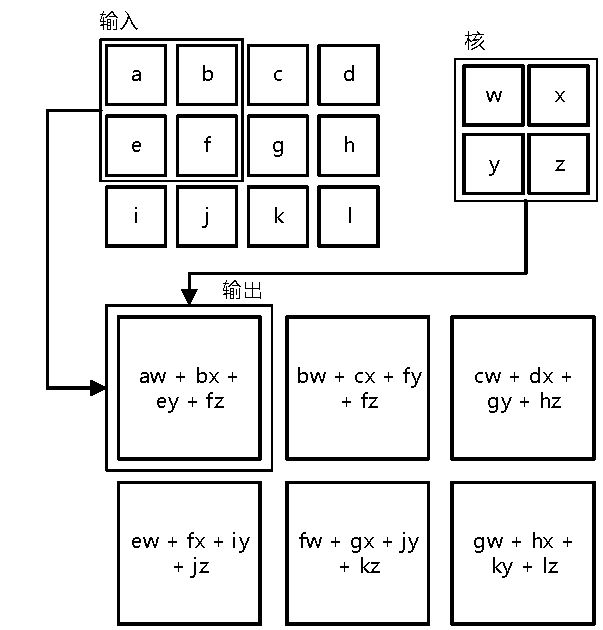
\includegraphics[width=0.4\textwidth]{figure/convolution-process.pdf}
  \bicaption
    {卷积过程}
    {Convolution process}
  \label{fig:convolution-process}
\end{figure}
演示了一个在二维张量上的卷积运算过程。稀疏交互、参数共享和等变表示是卷积运算中的三个思想,三个思想之间互相影响,卷积神经网络只需要较少的模型参数便能实现可靠地特征提取。池化函数使用某个位置的相邻输出的总体统计特征来代替网络在该位置的输出,可对输入进行降维,为神经网络提供了某种程度平移不变性,常用的池化函数有最大池化函数、平均池化函数等。


\section{本章小结}
本章是手写签名认证相关技术的分析,首先分别从手写签名认证中的感知技术和手写签名认证中的建模方法两个方面对现有的研究进行了综述,然后分析总结了现有研究存在的问题。基于存在的问题,提出了本文的技术路线,最后介绍了本文中所涉及到的相关理论和技术。

\chapter{基于声波的签名认证方案的关键技术研究}
\section{问题描述与方案设计}
\subsection{问题描述}
本文要解决的问题是利用声波的相位相关信息实现手写签名认证,提出了一种基于声波的一个非侵入式、用户友好、安全、低延迟、准确的在线签名认证方案。其中需要考虑的几个关键的技术问题是音频设备硬件补偿技术技术问题、基于声波的相位相关信息的感知技术问题、基于声波的相位相关信息的特征提取技术问题以及基于声波特征的建模技术问题。基于智能手机产品设计实现了一个手写签名认证系统,并在实际场景下部署测试了该系统。

本文列举两个签名认证的例子来描述应用场景,场景一描述生活中在银行柜台取款的常见场景便于理解手写签名认证系统的实际作用,场景二则描述了本文所设计系统的可应用场景:

\textbf{(1)场景一}

一位叫波波的小伙子去银行取存款,申明他是某个存款账户的拥有者,银行职员要求他签名以便进行下一步操作。根据银行的实际情况,小伙子可能会在一张普通的纸上签字也可能在一个手写平板上签字。接着手写签名认证系统运行:首先它从数据库中查询了之前该小伙子留下的参考签名;接着它使用设定的算法比较查询签名和参考签名,计算出查询签名和参考签名之间的相似度。如果系统实时运行的话,银行职员根据签名认证系统的输出结果进行下一步操作。显然,对于基于普通纸张的签名,一个静态的图像将会从纸张上扫描所得,此时签名认证系统为离线签名认证系统;然而,基于手写平板的签名,一个额外的时间信息通常被用于提交认证的进度,此时的签名认证系统为在线认证系统。

\textbf{(2)场景二}

本文的签名认证方案可以作为一种需要和其他认证方案相结合的辅助认证方案,例如可以和现有的离线签证认证系统或者人工签名认证相结合,最终的系统利用多模的优势提高签名认证的精度。如图~\ref{fig:sign-senario}
\begin{figure}[!htp]
  \centering
  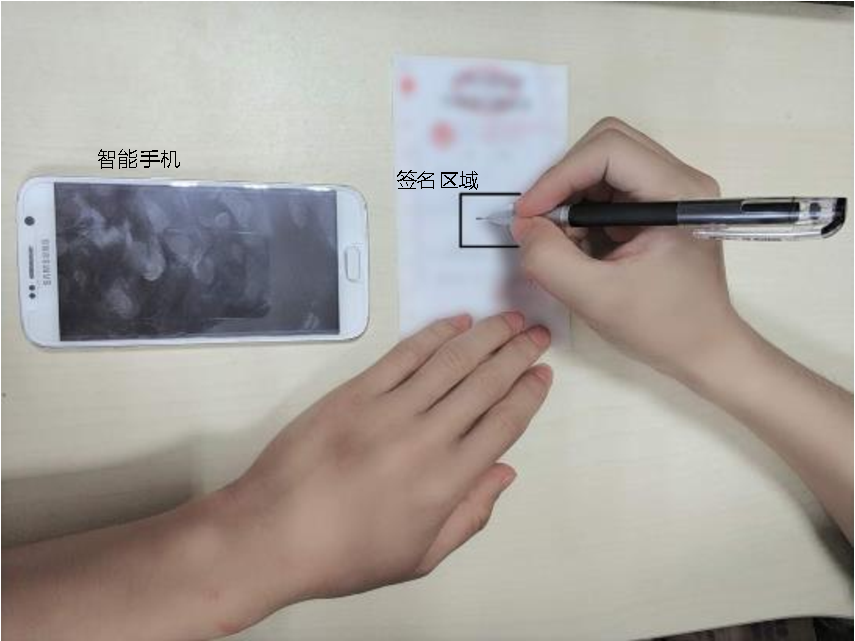
\includegraphics[width=0.4\textwidth]{figure/acoustic-senario.pdf}
  \bicaption
    {签名场景}
    {Senario of signing}
  \label{fig:sign-senario}
\end{figure}
所示,当一个人在一张现金支票上的签名区域签名时候,将他/她的智能手机放在签名区域旁边记录手和笔在签名动作过程中的模式,该模式将会发送到银行进行识别;纸上的签名将被扫描作为离线签名认证系统的输入;两种签名认证方案使用不同的权重,进行融合。可在支票打印一个二维码,通过二维码可以把智能手机获得签名模式和这张支票联系起来。


在两个场景中,默认参考签名已经预先被系统记录下。场景二是本文系统所适用的场景,签名者来的操作包括:获取支票、寻找签名区域、拿笔准备写、开启声波跟踪、开始手写、结束手写、结束声波跟踪、获得验证结果,如图~\ref{fig:signing-steps}所示。智能手机可以在场景中使用声波跟踪签名过程中手和笔的运动模式。然而使用智能手机收发声波跟踪手和笔运动实现在线认证的方案仍然面临着诸多挑战:首先,个人的签名仍然可以被观察和练习,这是目前所有签名认证系统所面临和需要克服的挑战;另外,声波可以被其他恶意的音频接收设备所接收,之后再播放出来实行重放攻击。
\begin{figure}[!htp]
  \centering
  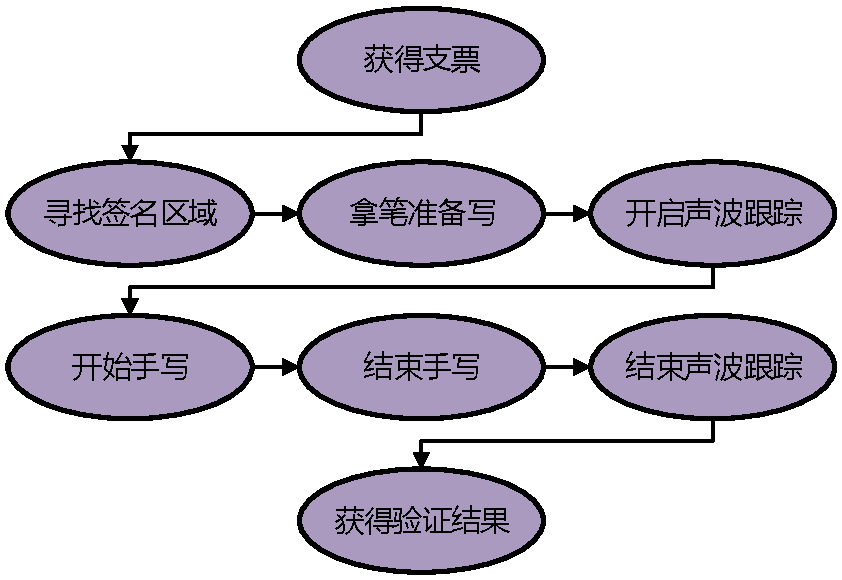
\includegraphics[width=0.5\textwidth]{figure/senario-actions}
  \bicaption
    {场景二签名步骤}
    {Signing steps in Senario 2}
  \label{fig:signing-steps}
\end{figure}

\subsection{方案设计}
针对上述问题,本文设计提出了一种基于声波的签名认证方案,如图~\ref{fig:acoustic-hsv-method}所示。该方案主要将声波感知技术引入到手写签名认证的研究中,包含四个关键步骤:声波收发、声波相位相关信息采集、特征提取、分类模型。
\begin{figure}[!htp]
  \centering
  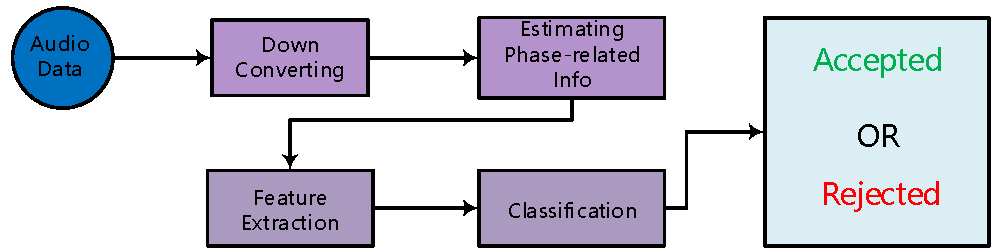
\includegraphics[width=0.6\textwidth]{figure/system-architecture.pdf}
  \bicaption
    {基于声波的手写签名认证方案}
    {Acoustic-based handwritten signature verification method}
  \label{fig:acoustic-hsv-method}
\end{figure}

(1) 声波收发

在发射声波之前,首先需要设计使用扬声器发射的音频文件,这个音频文件的设计需要考虑用户体验、系统可用性、系统鲁棒性这些特点,而且还需要适配扬声器的硬件特性,进行相应的硬件补偿。


(2) 声波相位相关信息采集

在收到声波反射信号之后,对声波信号进行向下转换从而获得基带信号的两个正交分量。通常在求相位之前,需要对这两个正交分量去直流,然后计算出相位信号,但是在这两个正交信号变化过于多样时,去直流变得异常困难。本文提出使用求弦长的方法,估算了相关信息(速度和加速度)。除了解决去直流问题,还需要预先对两个正交信号进行去噪。


(3) 特征提取

尽管声波的相关信息是经过降采样的,它的数据量仍然较大,不宜直接进行分类。本步骤对信号进行频域分析并做余弦变换,选择低频信息作为特征,并计算查询签名与参考签名之间的距离矩阵。

(4) 分类模型

本文采用CNN作为二分类的分类模型。模型在调整好参数和使用一些防止过拟合的方法后,使用上一步骤中距离矩阵作为输入进行二分类,输出一个范围为0到1的概率值,输出值越大表明输入签名是真实签名的概率越大。

\section{音频设备硬件补偿技术的研究}\label{sec:audio-research}

本节先介绍原型系统ASSV中的声波信号的设计理念,然后针对设计好的声波信号结合智能手机采取硬件补偿的措施。

\subsection{声波信号的设计}

用于在智能手机上发射的声波实际上是使用扬声器播放一个按特定目的设计的音频信号,因此关于声波信号的设计实际就是关于音频文件中二进制数据序列的设计。为了使麦克风上接收的信号可分析,本文设计一种特定的声音让扬声器发射,在此设计中主要考虑三个方面:用户体验、系统可用性、系统鲁棒性。

\textbf{\textit{(a)} 声波信号设计需要考虑用户体验。}为了让系统提供用户友好型的交互和良好的用户体验,由智能手机发送的声波不应该是人耳可听见的。根据Rodr{\'\i}guez Valiente~\cite{rodriguez2014extended}的综述,当声波的频率高于17 kHz的时候,声音对人便变得不可听。因此,本文生成的声波的频率均大于17 kHz,而且这些声波均可以被商用音频设备(包括本文所用到的智能手机上的扬声器)发射。

\textbf{\textit{(b)} 声波信号设计需要考虑系统可用性。}与LLAP~\cite{wang2016device}中所发射的声波信号相似,为了测量随着传播路径变化的声波信号的相位,本研究生成声波信号的时候使用连续波(Continuous Wave, CW)信号:
$$
Acos2\pi ft, 
$$
其中$A$代表信号强度,而$f$代表信号频率。再则,ASSV使用同一个智能手机上的扬声器和麦克风来发射和接收声波,这两个音频设备在同一个智能手机上使用同一个时钟频率,所以不存在载频偏移问题。

\textbf{\textit{(c)} 声波信号设计需要系统鲁棒性。}本系统需要具有鲁棒性,即使多径效应丰富的环境下也能保持可用。如图~\ref{fig:signal-travel-paths}所示,将声波的传播路径分成4种类型:手和笔的反射路径、直接路径、静止路径和动态多径。
第一种类型,如图~\ref{fig:signal-path-pen-hand-reflected-path}所示,信号从扬声器发出,经过笔和手的反射,传播回到麦克风中。该路径长度随着手写动作的进行而发生变化,实际上,路径是跟踪签名活动中人行为特征的真正所需要的路径;
第二种类型,本文称这种路径为直接路径。如图~\ref{fig:signal-path-direct-path}所示,信号直接从扬声器传播到麦克风,没有经任何物体反射,因为直接传播路径使所有可能传播路径中最短的一条,所以从直接路径上传播的信号具有最大的能量,换而言之,具有最大的信号波振幅;
第三种类型,本文称这种路径为静止路径,如图~\ref{fig:signal-path-static-multipath}所示,声波仅仅被障碍物反射了一次,图中的障碍物可以是桌子、人的身体等一些在智能手机附近可以阻挡声音的障碍物,直接路径和静止路径传播的声波信号在本文被看作背景信号,手写签名过程中手和笔的运动并不能对背景信号产生丝毫影响;
第四种类型如图~\ref{fig:signal-path-dynamic-multipath}所示,声波信号从扬声器出发,经过手写过程中的手和笔的反射,再次经过障碍物的反射,最后才传播回到麦克风中,因为障碍物是不确定的,通常是由形状不规则的非结构化的物体组成,所以经过这种路径传播的声波信号总体上被认为是不稳定和不确定的。
\begin{figure}[!htp]
  \centering
  \begin{subfigure}[b]{0.49\textwidth}
    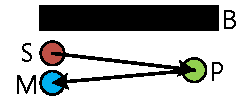
\includegraphics[width=\textwidth]{figure/signal-path-pen-hand-reflected-path}
    \caption{}
    \label{fig:signal-path-pen-hand-reflected-path}
  \end{subfigure}
  \begin{subfigure}[b]{0.49\textwidth}
    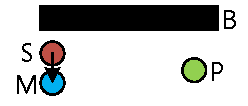
\includegraphics[width=\textwidth]{figure/signal-path-direct-path}
    \caption{}
    \label{fig:signal-path-direct-path}
  \end{subfigure}
  \begin{subfigure}[b]{0.49\textwidth}
    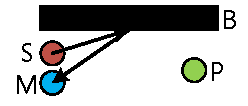
\includegraphics[width=\textwidth]{figure/signal-path-static-multipath}
    \caption{}
    \label{fig:signal-path-static-multipath}
  \end{subfigure}
  \begin{subfigure}[b]{0.49\textwidth}
    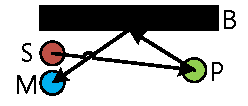
\includegraphics[width=\textwidth]{figure/signal-path-dynamic-multipath}
    \caption{}
    \label{fig:signal-path-dynamic-multipath}
  \end{subfigure}
  \bicaption[信号传播路径]
  {信号传播路径 - (a) 手和笔的反射路径; (b) 直接路径; (c) 静止路径; (d) 动态多径。\textbf{S}, \textbf{M}, \textbf{P}, \textbf{B} 分别代表 扬声器(\textbf{S}peaker), 麦克风(\textbf{M}icrophone), 笔(\textbf{P}en), 障碍物(\textbf{B}lock)。}
  {Signal traveling paths - (a) Hand and pen reflected path; (b) Direct path; (c) Static multipath; (d) Dynamic multipath. \textbf{S}, \textbf{M}, \textbf{P}, \textbf{B} represent \textbf{S}peaker, \textbf{M}icrophone, \textbf{P}en, \textbf{B}lock respectively.}
  \label{fig:signal-travel-paths}
\end{figure}


本文使用信号的指数形式来解释最终的接受信号。假设$x_{i}^{'}(t)=A_{i}^{'}e^{-a_{i}^{'}t},x_{j}^{''}(t)=A_{j}^{''}e^{-a_{j}^{''}t},x_{m}^{'''}(t)=A_{m}^{'''}e^{-a_{m}^{'''}t},x_{n}^{''''}(t)=A_{n}^{''''}e^{-a_{n}^{''''}t}$分别表示第一种类型、第二种类型、第三种类型、第四种类型路径的信号,其中$i,j,m,n$是正整数用于表示“其中一条路径”的意思。假设$X^{'}(t),X^{''}(t),X^{'''}(t),X^{''''}(t)$分别表示四种类型路径上信号的和,$I,J,M,N$分别代表四种类型路径集合中各自的路径数量,可以得到:
\begin{eqnarray}
X^{'}(t) &=\quad  \sum_{i=1}^{I}x_{i}^{'}(t)      &=\quad   \sum_{i=1}^{I}A_{i}^{'}e^{-a_{i}^{'}t}, \\ \label{eq:path-1}
X^{''}(t) &=\quad  \sum_{j=1}^{J}x_{j}^{''}(t)     &=\quad  \sum_{j=1}^{J}A_{j}^{''}e^{-a_{j}^{''}t}, \\ \label{eq:path-2}
X^{'''}(t) &=\quad   \sum_{m=1}^{M}x_{m}^{'''}(t)    &=\quad   \sum_{m=1}^{M}A_{m}^{'''}e^{-a_{m}^{'''}t} ,\\ \label{eq:path-3}
X^{''''}(t) &=\quad   \sum_{n=1}^{N}x_{n}^{''''}(t)  &=\quad   \sum_{n=1}^{N}A_{n}^{''''}e^{-a_{n}^{''''}t}. \label{eq:path-4}
\end{eqnarray}
$X(t)$表示麦克风接收的信号,则可以得到:
\begin{equation}
\begin{aligned}
X(t)=X^{'}(t) + X^{''}(t) + X^{'''}(t)+ X^{''''}(t). \label{eq:path-total}
\end{aligned}
\end{equation}
将式~\ref{eq:path-1}、式~\ref{eq:path-2}、式~\ref{eq:path-3}和式~\ref{eq:path-4}代入式~\ref{eq:path-total}中,可以得到:
\begin{equation}
\begin{aligned}
X(t)=\sum_{i=1}^{I}A_{i}^{'}e^{-a_{i}^{'}t} + \sum_{j=1}^{J}A_{j}^{''}e^{-a_{j}^{''}t} +\sum_{m=1}^{M}A_{m}^{'''}e^{-a_{m}^{'''}t}+ \sum_{n=1}^{N}A_{n}^{''''}e^{-a_{n}^{''''}t}. \label{eq:path-total-final}
\end{aligned}
\end{equation}

式~\ref{eq:path-total-final}中第一项是本研究所关心可用于跟踪手写行为的变量,第二项与第三项可以认为是常量,第四项是不稳定变化的。第二项和第三项可以通过作差法去除。第四项是在设计声波信号时需要着重考虑的。通常,结合来自不同频率上的信号的结果可以缓解第四种类型的传播路径最后对结果的影响,这种方法可以被用于提高轨迹跟踪或者活动识别的精度。

本文选择多个频率高于17 kHz的声波信号组成最后的发射信号。根据香浓采样定理,麦克风在采样频率为48 kHz时,可接收的声波频率不应高于24 kHz,实际由于硬件原因,这个上限会更小。看似所选用的不同频率的信号越多则越有利于缓解动态多径所产生的影响,但是实际上并不能这样做,这是因为频率越多,每个频率上的信号分得的能量便越小,能量减小导致信噪比下降。本文通过实验来解释这个现象,分两次发射不同的声波,第一次发生18 kHz声波,第二次发射 18 kHz 和 18.6 kHz的声波,每次发射3秒,取最后一秒利用快速傅里叶变换(Fast Fourier Transform, FFT)进行频域分析。如图~\ref{fig:frequency-analysis-one-frequency}和图~\ref{fig:frequency-analysis-two-frequency}所示,
\begin{figure}[!htp]
  \centering
  \begin{minipage}[t]{0.49\textwidth}
    \centering
    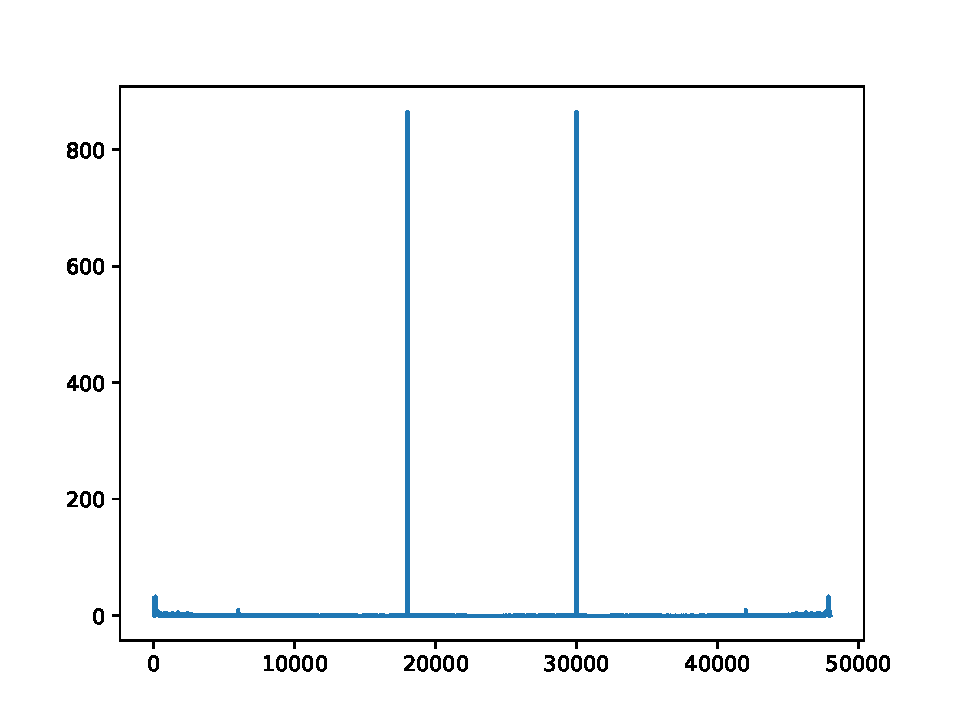
\includegraphics[width=\textwidth]{figure/one-freq-fft.pdf}
      \bicaption{单频率声波频域分析}
      {Frequency analysis on one-frequency sound}
        \label{fig:frequency-analysis-one-frequency}
  \end{minipage}
  \centering
  \begin{minipage}[t]{0.49\textwidth}
    \centering
    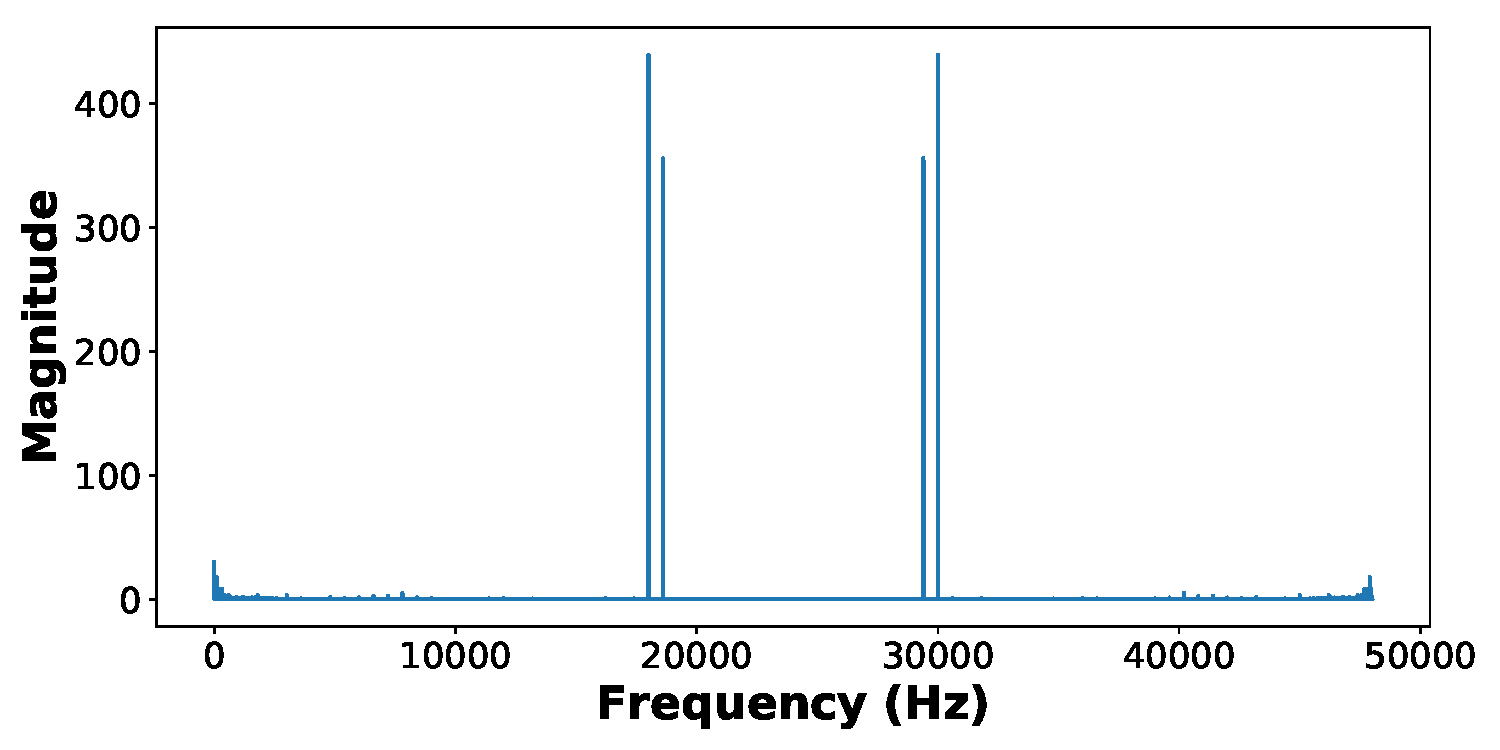
\includegraphics[width=\textwidth]{figure/two-freq-fft.pdf}
    \bicaption
    {双频率声波频域分析}
    {Frequency analysis on two-frequency sound}
    \label{fig:frequency-analysis-two-frequency}
   \end{minipage}
\end{figure}
双频率声波的18 kHz和18.6 kHz频率上的能量相加才是单频声波的18 kHz频率上的能量。本文采用8个频率合成发射声波,在研究中所选的频率集合$S_{freq}$可以表示为:
\begin{equation}
  S_{freq}=  \left\lbrace f | f=17350+700i, i \in \left[ 0,7 \right] \cap \mathbb{N} \right\rbrace.
\end{equation}
其中,8个频率开始频率为17350 Hz,每个频率所占频带和抗干扰保护频带分别为200 Hz和500 Hz。8个不同频率的信号被计算并标准化到取值范围$[-1,1]$,如下所示:
\begin{equation}
  Signal=\frac{1}{|S_{freq}|}\sum_{f \in S_{freq}}cos 2\pi ft.
\end{equation}

\subsection{音频设备硬件补偿}
由于智能手机的扬声器不是专为声波感知而设计的,能量在不同频率的信号上不是均匀分布的,如图~\ref{fig:nocompensation}所示,
\begin{figure}[!htp]
  \centering
  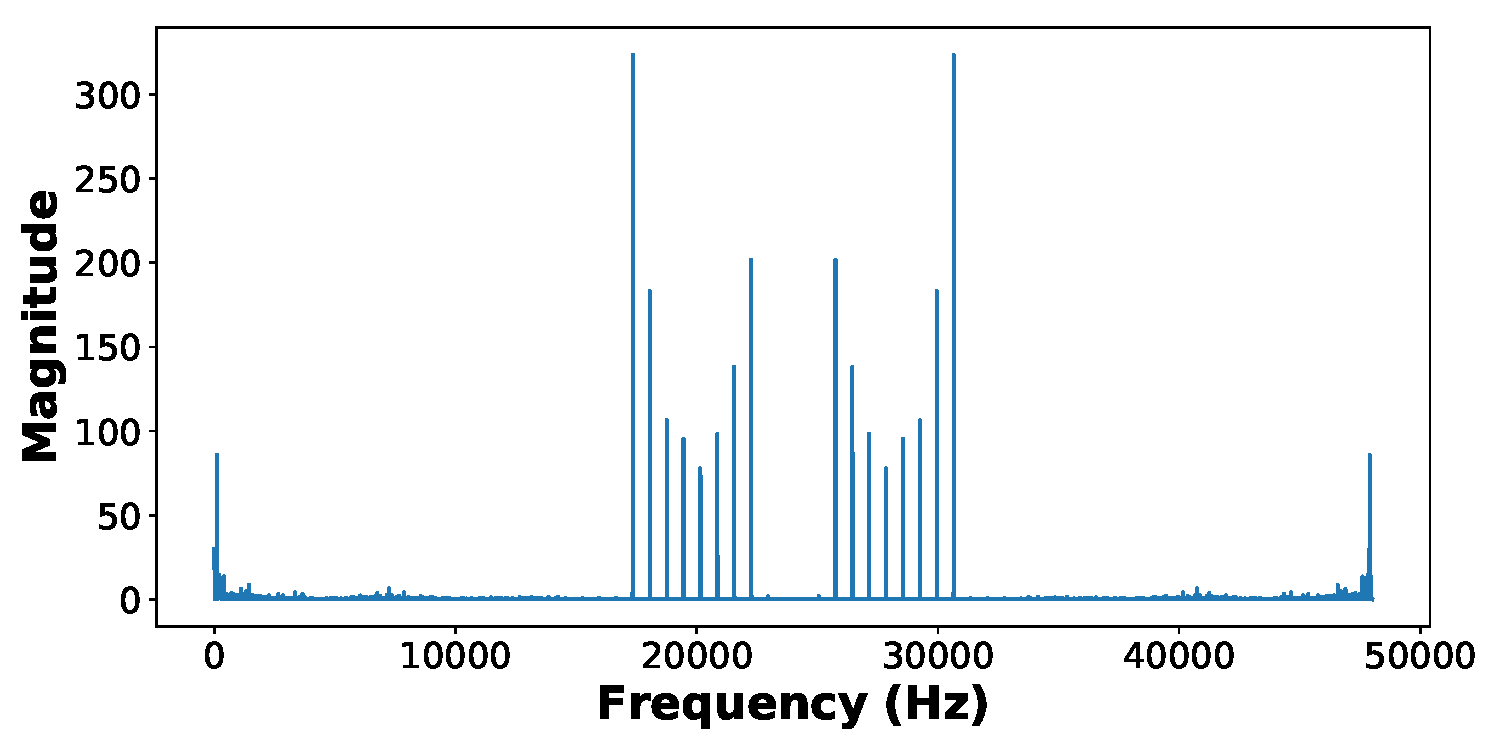
\includegraphics[width=0.6\textwidth]{figure/nocompensation.pdf}
  \bicaption
    {在硬件补偿之前的频域效果}
    {Frequency-domain effect without dardware compensation}
  \label{fig:nocompensation}
\end{figure}
通过对1秒时间的接收信号进行傅里叶变换,观察到有些频率上的信号能量十分小,而有些频率上的信号能量比较大。由于低能量的信号会导致低信噪比(signal-to-noise ratio, SNR),本文需要使用针对音频设备硬件的补偿技术:

(1)发射声波信号$Signal$ 5秒钟,挑选出第3秒这一秒的数据序列,这个数据序列在采样率为48 kHz的情况下一秒的数据有48000个数据点。

(2)对所选的数据序列进行傅里叶变换,从而获得所选频率上的幅度。假设$f_{i} = 17350 + 700i$代表第$i$个频率,$A_{i}$代表对傅里叶变换所得复数系数进行$abs$操作,$abs$是一个Python中计算绝对值的函数。

(3)将发射声波$Signal$替换为:
\begin{equation}
Signal_{compensated}=\alpha \sum_{i=0}^{|S_{freq}|-1} \frac{1}{A_i} cos 2\pi f_{i}t.
\end{equation}
其中$\alpha$是幅度缩放系数以保证$\alpha \sum_{i=0}^{|S_{freq}|-1}\frac{1}{A_i}=1$。

\section{基于声波的相位相关信息的感知技术研究}\label{sec:sensing-research}
为了获得接收声波中的相位相关信息,需要先对接收信号进行下转化(signal down conversion),然后根据获得的两个正交分量计算相位相关信息。

\subsection{信号下转化}
在计算相位相关信息之前,首先需要对接收信号进行信号下转化,将信号从通带信号(passband signal)转化为基带信号(baseband signal),这个过程在LLAP~\cite{wang2016device}中有所描述,本文重点描述与其的不同之处。

为了易于实现ASSV,本文使用巴特沃斯低通滤波器(low-pass Butterworth filter)作为所需的低通滤波器,而不是Cascaded Integrator Comb (CIC)滤波器。不失一般性,本文首先描述单一频率声波信号的信号下转化过程,如图~\ref{fig:sound-signal-down-conversion}所示。在此过程中,接收信号分两个分支进行操作:其中一个分支中,接收信号乘以$cos2\pi ft$并紧跟一个低通滤波操作,获得基带信号的同相分量(In-phase, I);另外一个分支中,接收信号乘以$-sin2\pi ft$并紧跟一个低通滤波操作,获得基带信号的正交分量(Quadrature, Q)。对两个分支经低通滤波获得的输出进行降采样,将数据量缩小到原来的$1/300$。既然在扬声器上的声波发射频率和麦克风上的声波接收频率均为48 kHz,所以最后数据的采样率是160 Hz,这其实是计算开销和判别准确性之间的一个折衷。


在实验的同时,有人在说话,有空调在运行,有个人电脑的散热器在转动,所以接收信号受到繁杂的环境噪声影响,如图~\ref{fig:noisy-denoised-component}所示,
\begin{figure}[!htp]
  \centering
  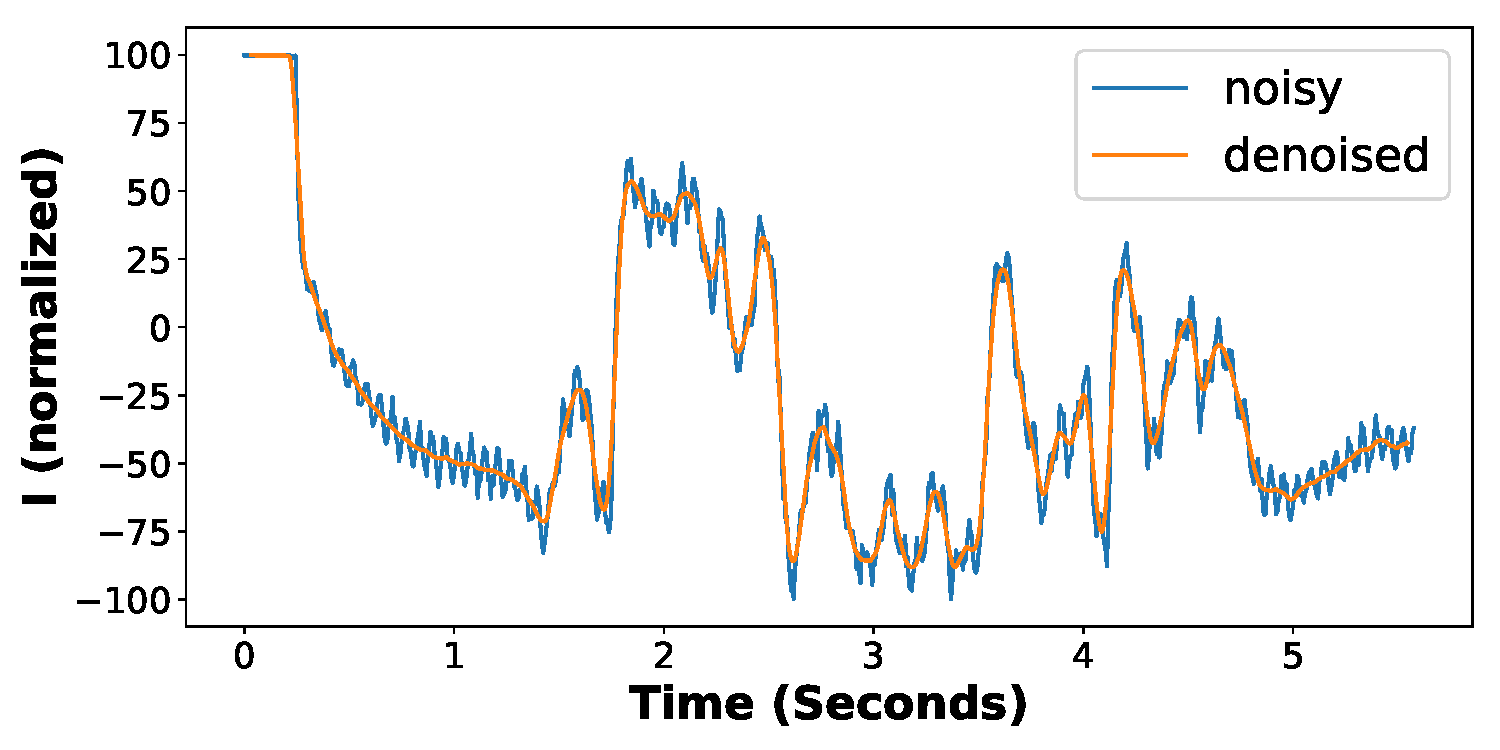
\includegraphics[width=0.6\textwidth]{figure/noisy-I.pdf}
  \bicaption
    {有噪声和去噪后的同相分量}
    {Noisy and denoised In-phase components}
  \label{fig:noisy-denoised-component}
\end{figure}
可以看到充满噪声的同相分量的曲线。虽然大多数噪声(比如人说话的声音)已经被低通滤波器所滤去,但是一些噪声仍然存在于基带信号中。在同相和正交分量中,可以发现一个周期性的噪声信号,此信号可以通过如下三个步骤进行测量:

(1)在没有手写动作影响的情况下,获得一段主要受到环境噪声影响的同相或者正交分量;

(2)使用一个基于函数的方法找出这段曲线中所有的波峰;

(3)计算两个波峰之间时间间隔的平均值,用于估算噪声的波动周期。

获得噪声信号的周期之后,本文直接在时域信号上使用另外一个基于函数的趋势季节分解(Trend-Seasonal Decomposition, STD)~\cite{cleveland1990stl}方法,该方法使用滑动平均的方式实现,目前有乘法STD和加法STD。在乘法STD中,原始序列为趋势序列、季节序列和残差序列之积,适用于季节的幅度随着时间变大而变大的情形;在加法STD中,原始序列为趋势序列、季节序列和残差序列之和,适用于季节的幅度不随着时间的变化而变化。STD函数要求输入一个周期,即使用波峰之间时间间隔估算出的周期,分解后之后可以获得三个序列:

a.趋势序列。趋势序列包含低频信号,本文中该低频信号随着手写动作的变化而变化;

b.季节序列。季节是一个周期性序列,其周期是调用STD时所输入的值;

c.残差序列。残差序列是一个这样的一个序列,为了满足相加模型:$Y[t] = T[t] + S[t] + e[t]$,其中,$Y[t]$代表原始序列,$T[t]$代表趋势序列,$S[t]$代表季节序列,$e[t]$为残差序列。

图~\ref{fig:trend-seasonal-decomposition-effect}展示分解效果,
\begin{figure}[!htp]
  \centering
  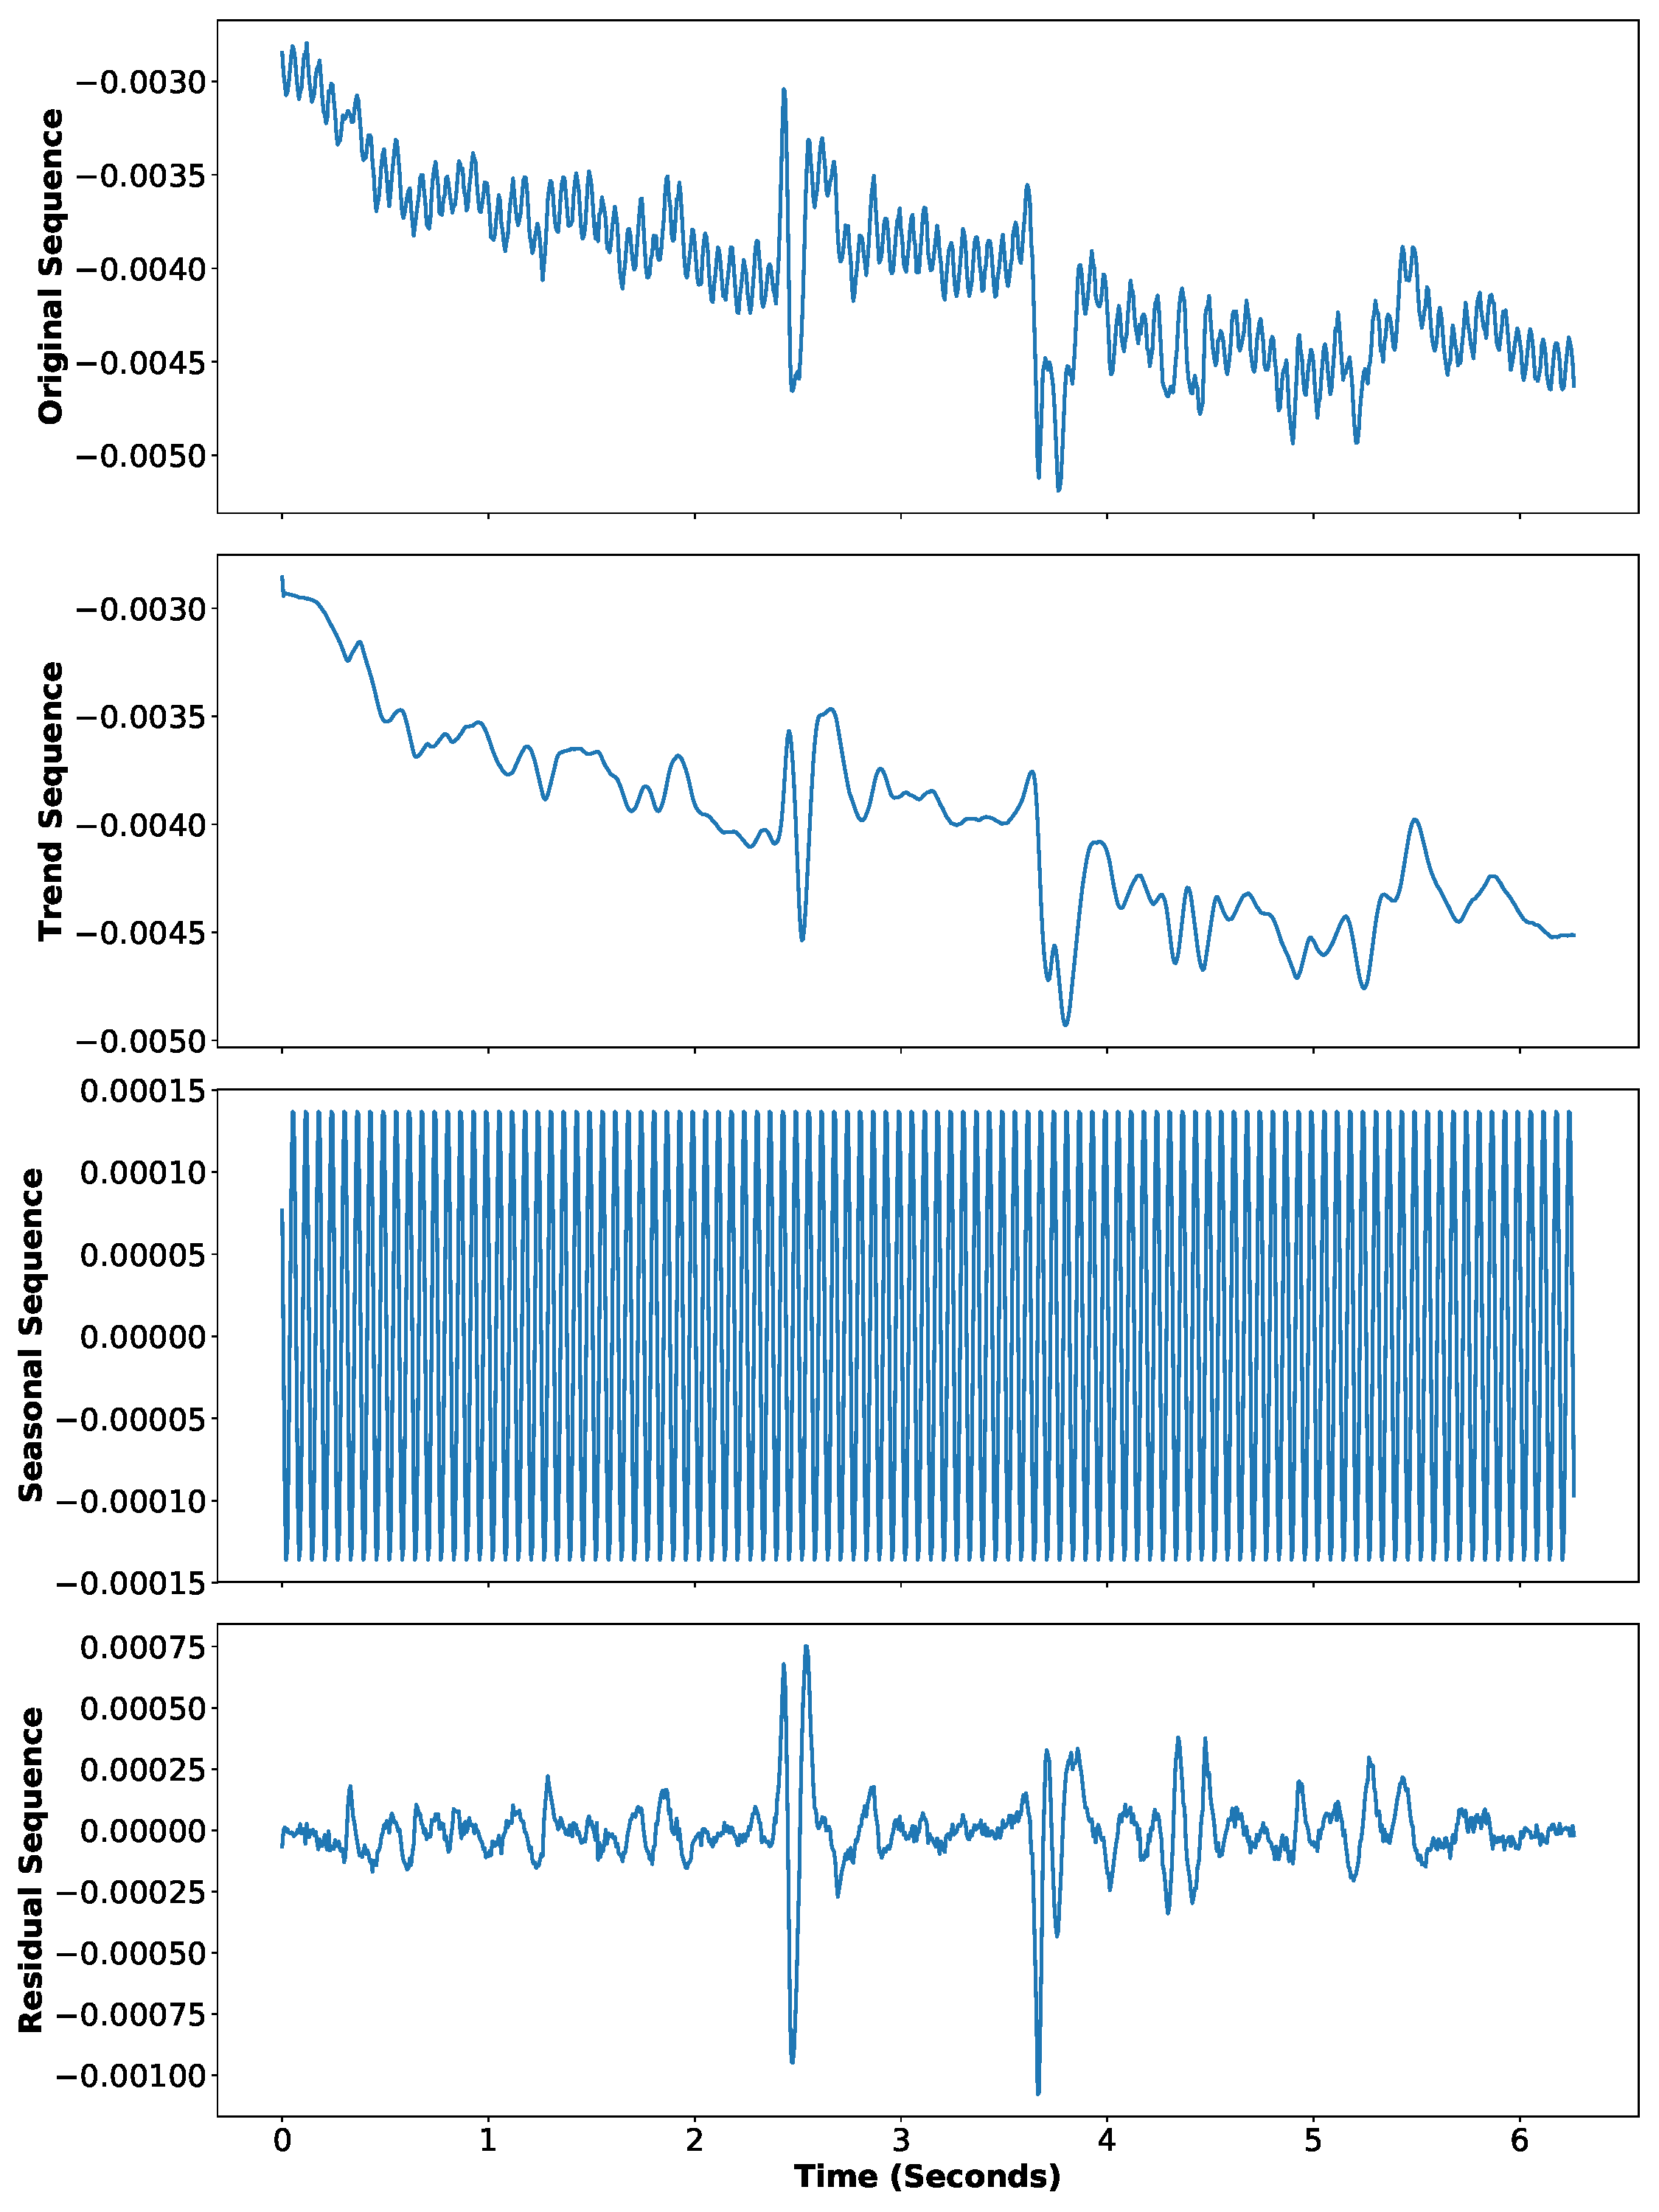
\includegraphics[width=0.55\textwidth]{figure/std-effect.pdf}
  \bicaption
    {趋势季节分解效果}
    {Trend-Seasonal Decomposition Effect}
  \label{fig:trend-seasonal-decomposition-effect}
\end{figure}
从上到下的子图分别是原始序列、趋势序列、季节序列和残差序列。在STD的输出序列中,本文只采用趋势序列作为结果序列,如图~\ref{fig:noisy-denoised-component}所示,充满噪声的是原始序列,而相对平滑的是趋势序列,该图展现STD在本文中良好的去噪声效果。

本文使用的是离线版本的STD,只有当声波信号被全部接收和下转化之后,STD才能对整个信号使用。既然该基于函数的方法使用滑动平均的方法,STD实际上可以被实现成在线版本STD2~\cite{std2},在线版本更适用于实际应用,可以减少延迟。

\subsection{计算相位相关信息}
为了更好地理解估计相位相关信息的方法,首先展示2个关键发现,然后使用它们的数学原理。

\textbf{第一个关键发现。}研究三种运动模式下的相位变化:(a) 在每个方向都有中等幅度移动的运动;(b)在每个方向都有较小移动的运动;(c)在每个方向只有较小幅度的移动。当智能手机上扬声器和麦克风启动,同相和正交分量的幅度从零开始持续增加到一个稳定的值,这个阶段在ASSV中大约持续1秒时间,正如图~\ref{fig:large-magnitude-movements}、图~\ref{fig:medium-magnitude-movements}和图~\ref{fig:small-magnitude-movements}中路径$O\rightarrow S$所示。这三幅图展示了三种运动模式下的I/Q变化轨迹,其中点C是运动轨迹的中心,而x轴和y轴分别代表同相分量(I-component)和正交分量(Q-component)。深入地分析这三幅图,如果点C为圆心,可以发现圆弧的度数就是相位的大小,为了计算这个度数,$C(x_{0},y_{0})$的位置需要从同相分量和正交分量的序列估计出来。

如图~\ref{fig:large-magnitude-movements}所示,对于每个方向上都有大幅度移动的运动模式,这种运动模式会造成相位在同一个方向(顺时针方向)上运动较长时间,在这种情况下$x_0$和$y_0$通过分别计算同相分量和正交分量的平均值而得到。
\begin{figure}[!htp]
  \centering
  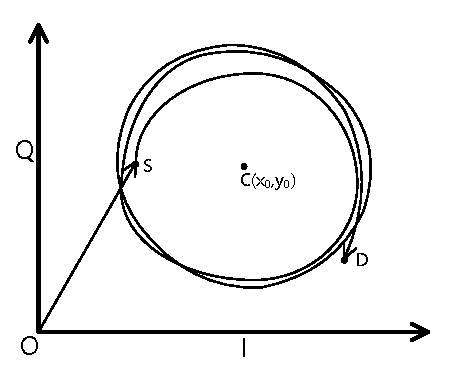
\includegraphics[width=0.5\textwidth]{figure/large-magnitude-movement.pdf}
  \bicaption
    {大幅度运动}
    {Large-magnitude movements}
  \label{fig:large-magnitude-movements}
\end{figure}

如图~\ref{fig:medium-magnitude-movements}所示,对于每个方向上都有中等幅度移动的运动模式,相位变化的方向变化较快,以致于同相分量和正交分量不是均匀分布,而是集中在\textit{Area 1},但是同相分量和正交分量的最小值和最大值还是达到了,对于这种情况,第一种情况中所使用的方法不再适用,但是仅仅依赖于最小值和最大值的方法LEVD~\cite{wang2016device}仍然可以工作得很好。
\begin{figure}[!htp]
  \centering
  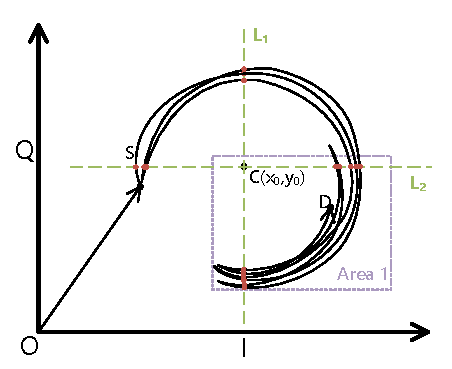
\includegraphics[width=0.5\textwidth]{figure/medium-magnitude-movement.pdf}
  \bicaption
    {中等幅度运动}
    {Medium magnitude movements}
  \label{fig:medium-magnitude-movements}
\end{figure}

如图~\ref{fig:small-magnitude-movements}所示,对于每个方向上的移动都是比较小的运动,相位的改变方向过于频繁,这种情况是手写运动中相位变化最常见的一种模式,在之前情况中所使用的方法将不适用,在这种情况下计算$x_{0}$和$y_{0}$变得很有挑战性。
\begin{figure}[!htp]
  \centering
  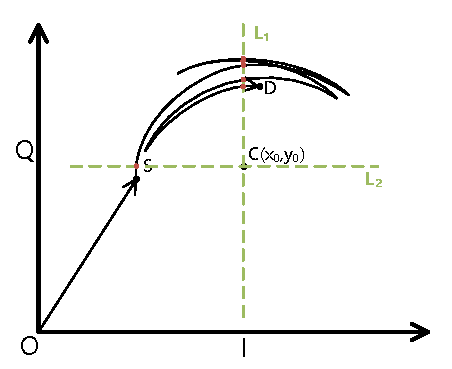
\includegraphics[width=0.5\textwidth]{figure/small-magnitude-movement.pdf}
  \bicaption
    {小幅度运动}
    {Small magnitude movements}
  \label{fig:small-magnitude-movements}
\end{figure}

\textbf{第二个关键发现。}研究了相位和弦长度变化之间的关系,对于半径一定的圆,越大的弦长意味着越大的圆心角,而圆心角在本文中就是相位(图~\ref{fig:large-magnitude-movements}、图~\ref{fig:medium-magnitude-movements}和图~\ref{fig:small-magnitude-movements})。基于这个观察,一个衡量弦长变化的方法被提出用于估量相位相关的信息,而非直接计算相位。

假设$Q[t]$和$I[t]$分别是正交分量和同相分量序列,其中$t=1,2,3,...,n$。图~\ref{fig:discrete-point-trace}展示
\begin{figure}[!htp]
  \centering
  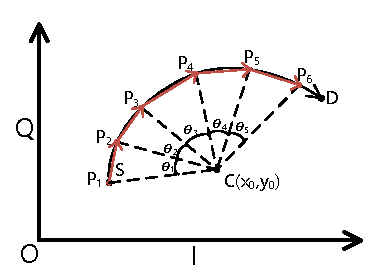
\includegraphics[width=0.5\textwidth]{figure/estimation-geometry.pdf}
  \bicaption
    {I/Q估计的上离散点}
    {Discrete points on the I/Q trace}
  \label{fig:discrete-point-trace}
\end{figure}
了$I[t]$和$Q[t]$的二维形状。$P_k$是一个在I/Q轨迹上的离散点,它的坐标是$(I[t],Q[t])$,其中$k=1,2,...,n$。$\theta_{k}$是对应于弦$P_{k}P_{k+1}$的圆心角。既然半径在很短的时间变化很小(在ASSV中为6 ms),可以得出:
$$
\begin{cases} 
  \theta_{k} \leq \theta_{k+1}, & \text{for } P_{k}P_{k+1} \leq P_{k+1}P_{k+2}  \\
  \theta_{k} > \theta_{k+1},  & \text{for } P_{k}P_{k+1} > P_{k+1}P_{k+2}
\end{cases}
.
$$
所以弦长的变化可以用于计算相位的变化。进一步,假设半径为$r$,使用数学方法证明这个推理,使其更有说服力:
\begin{align}
\Delta Chord_{k,k+1} &= \left\|P_{k+1}P_{k+2}\right\| - \left\|P_{k}P_{k+1}\right\|  \\ \label{eq:phase-approx}
&= 2rsin\frac{\theta_{k+1}}{2} - 2rsin\frac{\theta_{k}}{2} \nonumber \\  
&= 2r\left(sin\frac{\theta_{k+1}}{2} - sin\frac{\theta_{k}}{2}\right)  
.
\end{align}
利用$sin$的泰勒展式的第一项,可以得到:
\begin{align}
   sin\frac{\theta_{k+1}}{2} \approx & \frac{\theta_{k+1}}{2} ,\label{eq:taylor-series1}\\ 
    sin\frac{\theta_{k}}{2} \approx & \frac{\theta_{k}}{2}. \label{eq:taylor-series2}
\end{align}
将式~\eqref{eq:taylor-series1}和式~\eqref{eq:taylor-series2}代入式~\eqref{eq:phase-approx},可以得到:
\begin{equation}
 \Delta Chord_{k,k+1} \approx r(\theta_{k+1} - \theta_{k})=r\Delta \theta_{k,k+1} \Rightarrow \Delta \theta_{k,k+1} \approx \frac{1}{r}\Delta Chord_{k,k+1}.  \label{eq:velocity}
\end{equation}
虽然半径$r$仍然是未知的,但是,考虑到当$r$保持相同的时候,$\Delta \theta_{k,k+1}$和$\Delta Chord_{k,k+1}$成正相关变化。因为$\Delta Chord$序列和相位变化的速度相关,所以相位变化相关的加速度可以通过计算$\Delta Chord$的导数而进一步获得:
\begin{equation}
Acceleration_{k} = \frac{\left( \Delta Chord_{k,k+1} - \Delta Chord_{k-1,k} \right) + \left( \Delta Chord_{k+1,k+2}- \Delta Chord_{k-1,k}\right)/2}{2}. \label{eq:acceleration}
\end{equation}
相比只用两个点的计算方法,这种估计方式更具有鲁棒性。
既然$\left\|P_{k}P_{k+1}\right\|$在ASSV中可以被计算为:
\begin{equation}
  \left\|P_{k}P_{k+1}\right\|= \sqrt{\left( I[k+1] - I[k] \right)^2 + \left( Q[k+1] - Q[k] \right)^2}
\end{equation}
相似地,计算$\left\|P_{k+1}P_{k+2}\right\|$,然后将$\left\|P_{k}P_{k+1}\right\|$和$\left\|P_{k+1}P_{k+2}\right\|$代入式\eqref{eq:velocity}中,使用估计所得的$\Delta Chord $和式~\eqref{eq:acceleration},$Acceleration$可以被计算得到。



\section{基于声波的相位相关信息的特征提取技术研究}
\subsection{使用DCT的动机}
经过上一步,可以获得声波信号的基带信号,里面包含了签名运动的信息。此基带信号的采样率为160 Hz,如果按一次签名6秒时间算,则一个频率上会获得960个数据点,8个频率上总共上7680个数据点,直接使用这7680个数据点进行分类,会导致分类器难以收敛,分类效果不佳。本文采取对时域信号进行频域分析,签名运动的信息通常被认为是包含在低频信号里,而噪声信息则存在于高频信号中。时频转换的常见方法有:离散小波变换(Discrete Wavelet Transform, DWT)、离散傅里叶变换(Discrete Fourier Transform, DFT)和离散余弦变换(Discrete Cosine Transform, DCT)~\cite{安霄霄手写签名的多重数字水印及认证算法研究}。


小波变换~\cite{chun2010tutorial}和短时傅里叶变换(Short-time Fourier Transform, STFT)具有相似之处,都可以获得时域和频域信息。如图~\ref{fig:stft}所示,
\begin{figure}[!htp]
  \centering
  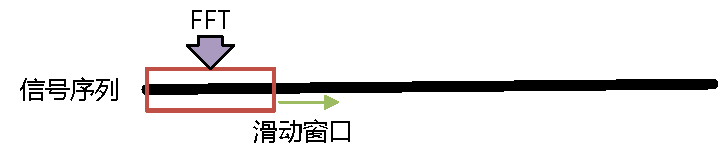
\includegraphics[width=0.7\textwidth]{figure/stft.pdf}
  \bicaption
    {短时傅里叶变换}
    {Short-time Fourier transform}
  \label{fig:stft}
\end{figure}
STFT使用一个滑动窗口,对窗口内的信号做快速傅里叶变换(Fast Fourier Transform, FFT),从而获得时域信息和频域信息用于绘制频谱图,了解频率随时间的变化情况,其中滑动窗口大小和窗口移动步长可以进行设置。然而窗口的大小限制了离散傅里叶变换的频率分辨率,离散小波变换能更好地解决这个问题。可以通过以下方式估计一个$f[n] \in l_{2}(Z)$:
\begin{equation}
f[n] = \frac{1}{\sqrt{M}}\sum_{k} W_{\phi}[j_{0},k]\phi_{j_{0},k}[n] + \frac{1}{\sqrt{M}}\sum_{j=j_{0}}^{\infty}\sum_{k}W_{\phi}[j,k]\phi_{j,k}[n].
\end{equation}
其中,$f[n]$,$\phi_{j_{0},k}[n]$ 和 $\phi_{j,k}[n]$ 是定义域为$[0,M-1]$,总共$M$个点的离散函数。集合$\{\phi_{j_{0},k}[n]\}$和集合$\{\phi_{j,k}[n]\}_{(j,k)\in Z^{2}, j \geq j_{0}}$相互正交,所以可以通过求内积的方式获得小波系数:
\begin{align}
W_{\phi}[j_{0},k]=&\frac{1}{\sqrt{M}}\sum_{n}f[n]\phi_{j_{0},k}[n]. \label{eq:approximation-efficients} \\
W_{\psi}[j,k] =& \frac{1}{\sqrt{M}}\sum_{n}f[n]\psi_{j,k}[n],  j \geq j_{0}. \label{eq:detailed-efficients}
\end{align}
式~\ref{eq:approximation-efficients}是近似系数,而式~\ref{eq:detailed-efficients}是细节系数。近似系数中包含低频信息,而细节系数包含高频信息,如图~\ref{fig:dwt}所示,原始信号经过小波变换可以得到近似系数和细节系数,而对近似系数和细节系数不断进行小波变换,从而得到想要的那段频率范围内的信息。
\begin{figure}[!htp]
  \centering
  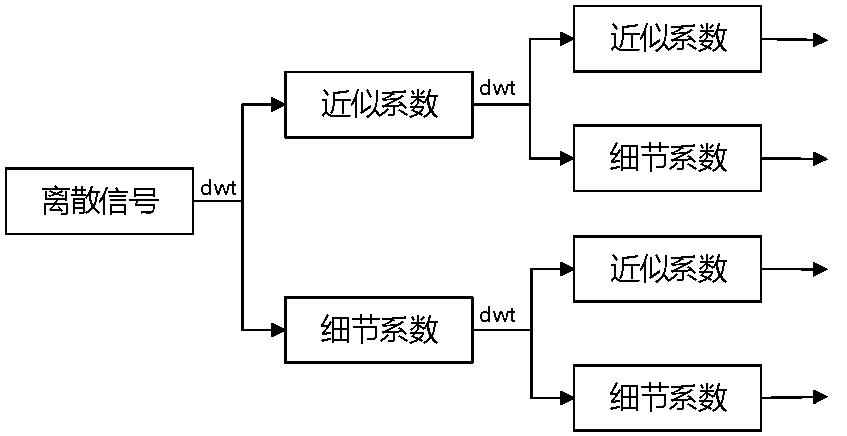
\includegraphics[width=0.5\textwidth]{figure/dwt.pdf}
  \bicaption
    {小波变换}
    {Discrete wavelet transform}
  \label{fig:dwt}
\end{figure}

离散傅里叶变换是常用的将时频变换的方法,假设$X_{k}$是信号的振幅序列,则傅里叶系数可通过以下的方式求得:
\begin{equation}
X_{k} = \sum_{n=0}^{N-1}x[n] \cdot e^{-j\frac{2\pi kn}{N}} \quad n=0,...,N-1.  \label{eq:dft}
\end{equation}
而离散傅里叶逆变换则是以下形式:
\begin{equation}
 x_{n} = \frac{1}{N}\sum_{k=0}^{N-1}X_{k} \cdot e^{j\frac{2\pi}{N}kn} \quad n=0,...,N-1. \label{eq:idft}
\end{equation}
从式~\ref{eq:idft}可以看出,计算DFT的时间复杂度为$O(n^{2})$,计算过程中存在很多重复的过程数据,快速傅里叶变换(Fast Fourier Transform, FFT)是离散傅里叶变幻的快速算法,将时间复杂度降为$O(nlog n)$。N个点的傅里叶变换的频谱分辨率为$\frac{2\pi}{N}$,这就解释了短时傅里叶变换的局限性:窗口越大傅里叶变换粒度变细,但是窗口数量减少,需要在时域信息和频域信息的多少之间进行权衡。傅里叶系数是复数系数,从式子~\ref{eq:dft}可知,第一个系数实际为所有数据点的和,傅里叶系数存在冗余。

离散余弦变换与傅里叶变换相关,最初的算法就提出了使用傅里叶变换实现余弦变换,余弦变换是一种无冗余系数的实数变换,详细参考~\ref{sec:dct}节。DCT的特点是前面系数包含低频信息,后面的系数包含高频信息,可以通过获取前几个系数来获得低频信息,不像离散小波变换需要经过多次变换才能获得所需的信息。因此,本文采用余弦变换用于特征提取和选择。

\subsection{特征矩阵和距离矩阵}  \label{sec:feature-distance-matrix}
在描述特征提取和选择过程之前,首先介绍两种矩阵:特征矩阵和距离矩阵。对于特征矩阵来说,每个手写签名都具有一个特征矩阵,这个矩阵包含所有提取和选择到的特征。对距离矩阵来说,它度量了查询签名和参考签名之间的相似度。通常认为,如果一个查询签名和相对应的参考签名具有较高的相似度,那么这个查询签名更有可能是一个真实签名,如果一个查询签名和相对应的参考签名具有较高的不相似度,那么这个查询签名更有可能是一个假签名。

对于每个接收的声波信号序列,因为在发送端有8个频率被使用到,因此可以获得8对 $\Delta Chord$和$Acceleration$序列。先将每个$\Delta Chord$或者$Acceleration$序列正规化到0-1的范围,然后采用DCT来获得信号的频域特征。DCT旨在实现数据的降维,它在信息包装和计算复杂度上有很好的权衡。不相关的DCT系数被产生,其中DCT系数的数量为输入序列的数据点数,前几个DCT系数通常被选取,而通常包含噪声信息的高阶系数通常被删除。结果,每个不同长度的时间序列都可以被转化为固定维度的特征向量,对于每个速度序列和加速度序列,本研究经验性地选择前10个DCT系数。

(1)特征矩阵

假设$W$是对于每个用户的参考签名数量。考虑8个频率,则特征向量的数量为$16*W$,其中包括$8*W$速度特征向量和$8*W$个加速度特征向量。对于每个参考签名,有8个速度特征矩阵,一个由这8个速度矩阵组成的形状为(8,10)的特征矩阵可以表示为:
\begin{equation}
  M_{i}^{vel}=\left( m^{vel}_{i,j,k}\right)_{8\times10} \quad i=1,2,..,W.
\end{equation}
接下来计算:
\begin{align} 
   a_{j,k}^{vel} =& min\{m^{vel}_{i,j,k}|i=1,..,W\} \\
   b_{j,k}^{vel} =& max\{m^{vel}_{i,j,k}|i=1,..,W\} \\
   c_{j,k}^{vel} =& \frac{1}{W}\sum_{1}^{W}m^{vel}_{i,j,k},
\end{align}
进而得到三个矩阵:
\begin{align}
A^{vel} =& \left(a_{j,k}^{vel}  \right)_{8\times10} \label{eq:vel-feature-matrices-minimum}\\  
B^{vel} =& \left( b_{j,k}^{vel} \right)_{8\times 10} \label{eq:vel-feature-matrices-maximum}\\ 
C^{vel} =& \left( c_{j,k}^{vel} \right)_{8\times 10} ,  \label{eq:vel-feature-matrices-mean}
\end{align}
其中,矩阵~\ref{eq:vel-feature-matrices-minimum}是最小值矩阵,矩阵~\ref{eq:vel-feature-matrices-maximum}是最大值矩阵,矩阵~\ref{eq:vel-feature-matrices-mean}是平均值矩阵。

对于加速度序列有:
\begin{equation}
  M_{i}^{acce}=\left( m^{acce}_{i,j,k}\right)_{8\times10} \quad i=1,2,..,W.
\end{equation}

进而得到三个矩阵:
\begin{align}
A^{acce} =& \left(a_{j,k}^{acce}  \right)_{8\times10}  \label{eq:acce-feature-matrices-minimum} \\
B^{acce} =& \left( b_{j,k}^{acce} \right)_{8\times10}  \label{eq:acce-feature-matrices-maximum} \\
C^{acce} =& \left( c_{j,k}^{acce} \right)_{8\times 10} \label{eq:acce-feature-matrices-mean}
\end{align}
其中,矩阵~\ref{eq:acce-feature-matrices-minimum}是最小值矩阵,矩阵~\ref{eq:acce-feature-matrices-maximum}是最大值矩阵,矩阵~\ref{eq:acce-feature-matrices-mean}是平均值矩阵。

结果,每个注册用户都有一个保存在本地文件系统中的参考矩阵:
\begin{equation}
 S_{reference}=\left\{ a_{j,k}^{vel},b_{j,k}^{vel},c_{j,k}^{vel},a_{j,k}^{acce},b_{j,k}^{acce},c_{j,k}^{acce} \right\}.
\end{equation}

(1)距离矩阵

当收到一个需要进行验证的查询签名的时候,ASSV首先计算该签名的两个特征矩阵:$M^{vel}$ 和 $M^{acce}$,然后计算6个距离矩阵:
\begin{align}
M^{vel} -& A^{vel}  \label{eq:distance-1} \\
M^{vel} -& B^{vel}  \label{eq:distance-2} \\
M^{vel} -& C^{vel}  \label{eq:distance-3} \\
M^{acce} -& A^{acce} \label{eq:distance-4} \\
M^{acce} -& B^{acce} \label{eq:distance-5} \\
M^{acce} -& C^{acce} \label{eq:distance-6}
\end{align}
结合式~\ref{eq:distance-1}、~\ref{eq:distance-2}、~\ref{eq:distance-3}、~\ref{eq:distance-4}、~\ref{eq:distance-5}和~\ref{eq:distance-6},获得一个三维的形状为$(8,10,6)$的矩阵,该矩阵将被作为分类模型的输入,用于训练和测试。

总而言之,特征矩阵用于进一步产生距离矩阵,而距离矩阵则被作为分类模型的输入。

\subsection{算法}
到目前为止,结合上文音频设备硬件补偿技术的研究~\ref{sec:audio-research}和基于声波的相位相关信息的感知技术的研究~\ref{sec:sensing-research},计算特征矩阵、参考矩阵和距离矩阵。算法~\ref{alg:get-feature-vector}(参见附录)用于计算特征向量。
基于算法~\ref{alg:get-feature-matrix}(参见附录),
可得出计算特征矩阵的算法。有了特征矩阵之后,可以计算参考矩阵,根据参考矩阵和查询签名的特征矩阵计算距离矩阵。

\section{基于声波特征的建模技术研究}
本文采用深度卷积神经网络作为二分类模型,相比传统机器学习分类器具有更优的分类性能。在距离矩阵经由计算得到后,一个二分类模型被训练用以判断给定的签名是否为真实签名,本文使用一个深度卷积神经网络以达到鲁棒的分类效果,该分类模型是一个用户独立的分类模型,当有新用户注册时,不需要重新训练模型。CNN是一种特殊的人工神经网络,旨在处理网格状的数据,它通常包含卷积操作和池化两类操作,图~\ref{fig:cnn-architecture}展示了本文设计的CNN模型。
\begin{figure}[!htp]
  \centering
  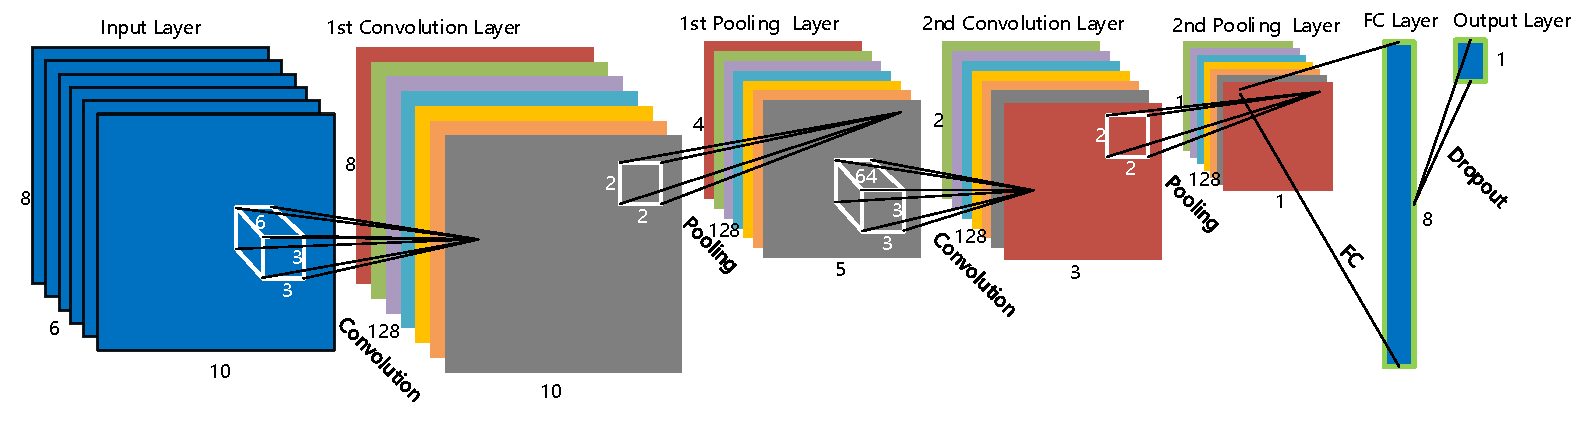
\includegraphics[width=\textwidth]{figure/cnn-architecture.pdf}
  \bicaption
    {CNN模型架构}
    {CNN achitecture}
  \label{fig:cnn-architecture}
\end{figure}

首先,距离矩阵作为一个三维张量输入第一层卷积层,该卷积层的激活函数是表达式为$max(0,x)$的\textit{RELU}。填充(padding)方式为\textit{SAME},用以保持输入尺寸与输出尺寸一样。第一层卷积层的输出被作为输入,输入到第一层池化层中,用以降采样操作,减小模型容量。池化层的输出作为下一层卷积池化层的输入。值得注意的是,每层卷积层的卷积核大小和数量被经验性地设为3和128,本文采用的池化类型为\textit{max pooling},这是一种最常用的池化操作,池化层的池化大小为2。虽然两重卷积池化层具有相似的配置,但是它们在模型中扮演着不同的角色:第一层卷积层旨在收集低层的特征信息,而第二层卷积层旨在收集较高层的特征信息。在选择卷积核数量的时候,本文在特征数量和计算开销之间进行了折衷,此外过多的卷积核更容易导致过拟合。


其次,最后一层卷积池化层的输出被铺平成一个向量。为了让CNN模型有更好的收敛速度,添加了一个批正规化层(Batch Normalization, BN)~\cite{ioffe2015batch},它不仅解耦了最后一层卷积池化层,而且保留了数据的表示能力。并且BN具有正则化的效果,不同小批之间差异性造成的随机噪声可以增加CNN模型的泛化性能。BN层的输出流入具有8个激活函数为\textit{RELU}的神经元的全连接层。为了进一步增加模型的泛化性能,采用了正则化的方法对核权重矩阵施加了一个$\alpha=0.001$的$L^2$的正则化,对全连接输出层施加了一个$\alpha=0.001$的$L^1$的正则化。此外,全连接层被施加了另外一个正则化技术,dropout~\cite{srivastava2014dropout},它通过以一定概率丢弃神经元来防止过拟合,本文经验性设置dropout rate为0.2。

最后,施加了dropout的输出被输入到输出层里,输出层只有一个激活函数为\textit{Sigmoid}的神经元,输出值的取值范围在0到1,代表了查询签名为真实签名的概率。与输出层的结构相对应地,二元交叉熵损失(binary cross entropy loss)被用于训练CNN模型。

\section{本章小结}
本章是基于声波的签名认证的关键技术研究,首先对要解决的问题进行了描述,然后提出一种基于声波的签名认证方案,该方案主要包含四个模块,对应了四种关键技术,依次对涉及到的音频设备硬件补偿技术、基于声波的相位相关信息的感知技术、基于声波的相位相关信息的特征提取技术和基于声波特征的建模技术进行深入研究,详细描述了方案中各模块的设计思想和技术细节。


\chapter{基于声波的签名认证方案的实验}
本章将对基于声波的签名认证方案进行实验验证以及分析。首先介绍在一定实验配置下的数据采集过程,然后展示评估实验及其相应的结果,这些评估实验包括:验证精度、交叉用户可用性、硬件补偿的效果、系统鲁棒性、微基准实验、对比实验和重放攻击。

\section{实验准备}
使用Kotlin语言开发了一个运行在安卓平台上的数据采集应用程序,将其安装在三星Galaxy S6上,使用主扬声器播放生成的WAV格式的音频文件,使用主麦克风接收声波。为了高效地采集数据,接收的声波数据首先保存在智能手机的本地存储空间里,等一个或者多个用户完成试验后,通过局域网传输到电脑上。所有分析过程和生成WAV文件的函数都使用Python语言实现,运行在电脑上用于分析和评估。CNN模型的训练和评估得到一台笔记本上的NVIDIA GeForce GTX 860M GPU的加速,这台笔记本还搭载了16GB RAM和一颗Intel Core i7-4710MQ 2.5GHz CPU。本研究实现了一个原型系统——ASSV,该原型系统由两部分组成1)一个安卓应用程序(apk大小:38.9 MB),执行的任务包括:数据采集、预处理和特征提取;2)一个运行在服务器上的分类器,它接收来自安卓应用程序的距离矩阵并返回结果。

志愿者受邀请到配合做实验,实验环境中有正在运行的空调、正在工作的电脑散热器和正在走路或者讲话的人员,实验环境,充满噪声,给系统带来了较大挑战。在做实验之前,每个志愿者会得到10分钟的训练,以熟悉采集程序并知道如何使用它。图~\ref{fig:app-ui}展示应用程序的用户界面,它支持的操作包括:开始采集,停止采集,输入保存接收的声波数据的文件名和路径上的两个目录名,删除所有的声音文件,以表格形式列出已经保存的声音文件,显示播放时间等。要求志愿者将智能手机放在一张经过精心设计的A4的纸上,该A4纸的每一面上包含28个签名区域,如图~\ref{fig:smartphone-setting}所示,
每个签名区域包含两条线段:一条9毫米长的分隔线段(separation line)和一条38毫米长的写线段(writing line),分隔线段的一端有一个十字,用于指引将智能手机的麦克风放在十字上方,并且它的底部边界与分隔线段和写线段所在的直线重合。在正确放置智能手机之后,志愿者按四个步骤在写线段上签名,如图所示~\ref{fig:data-collection}:
\begin{figure}[!htp]
  \centering
  \begin{minipage}[t]{0.32\textwidth}
    \centering
    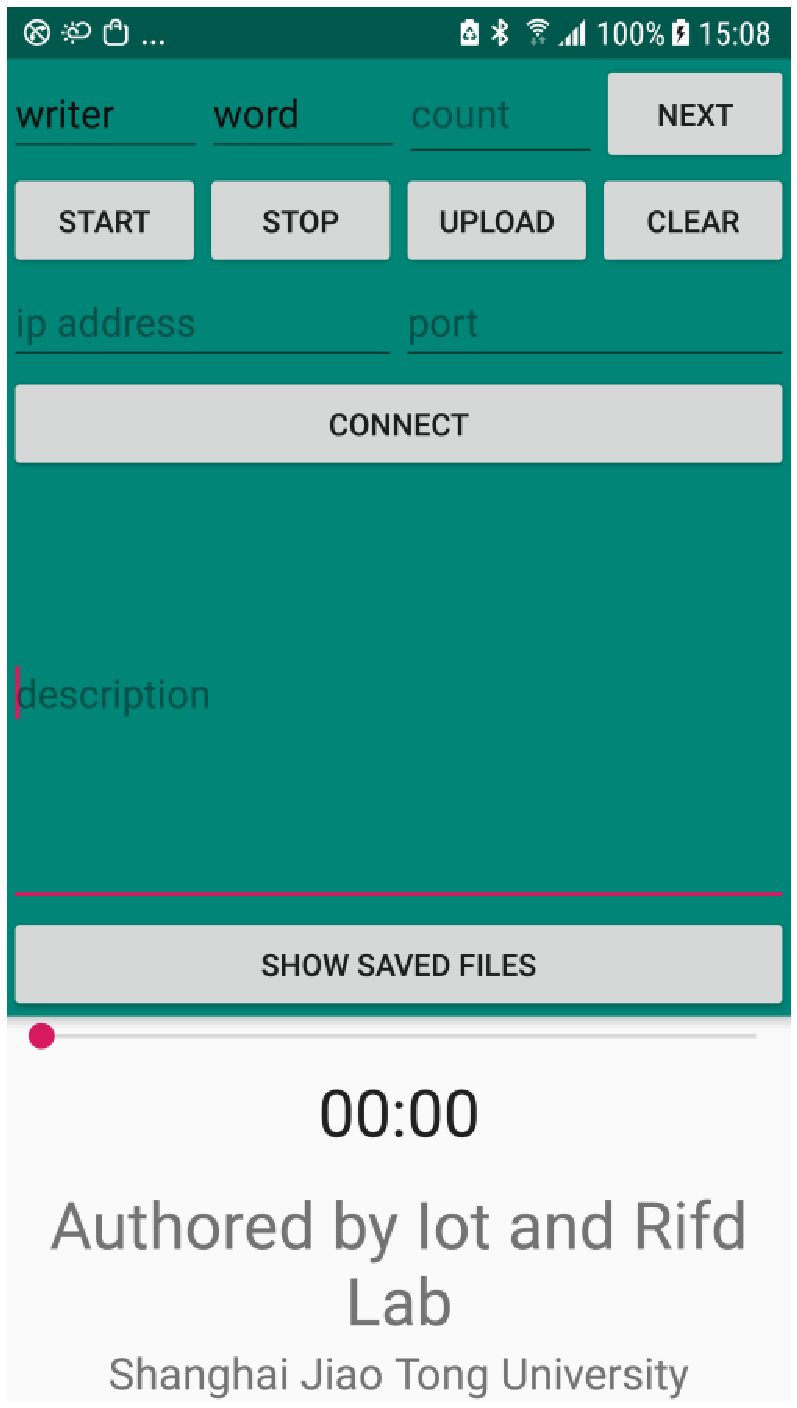
\includegraphics[width=\textwidth]{figure/app-ui.pdf}
      \bicaption{应用程序界面}
      {App UI}
        \label{fig:app-ui}
  \end{minipage}
  \centering
  \begin{minipage}[t]{0.32\textwidth}
    \centering
    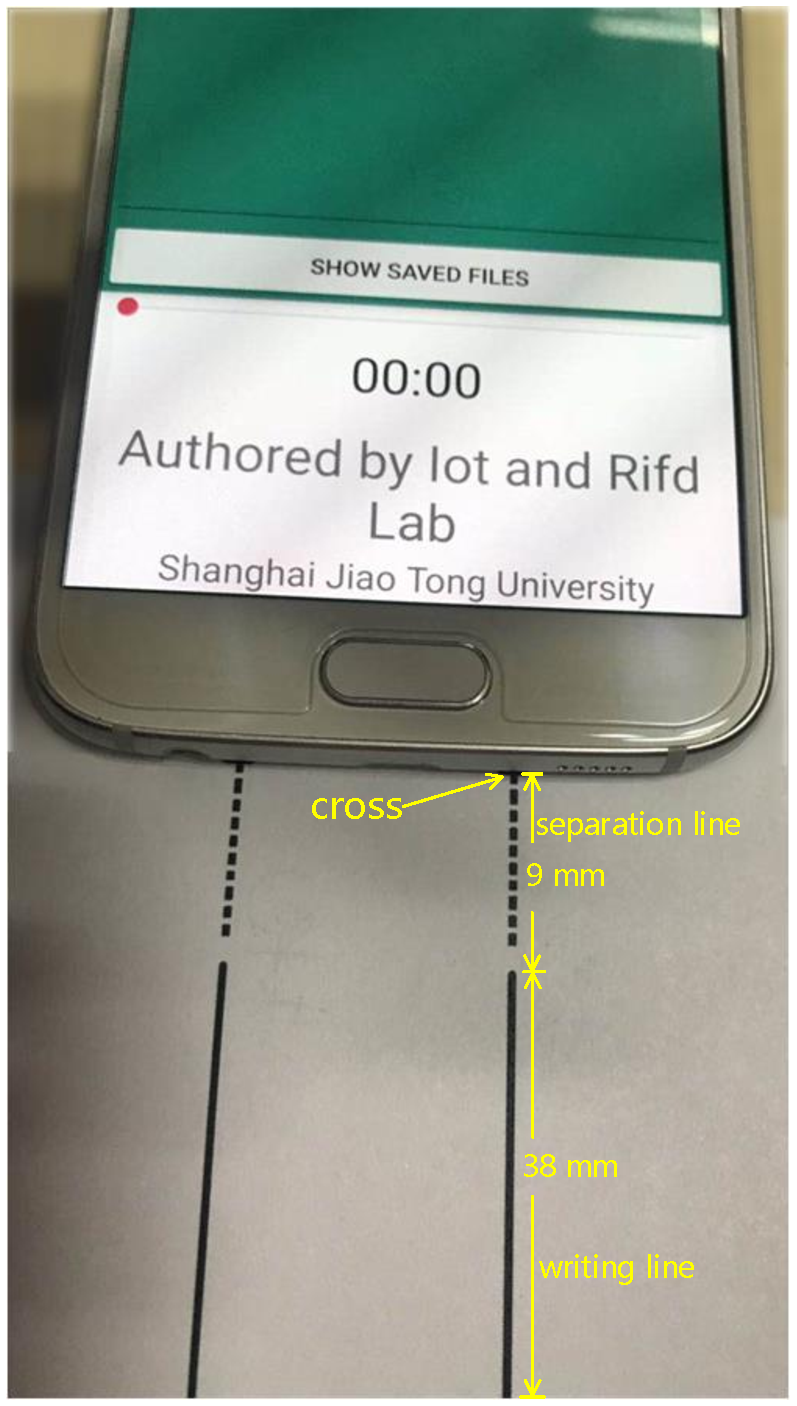
\includegraphics[width=\textwidth]{figure/app-smartphone-setting.pdf}
    \bicaption
    {智能手机设置}
    {Smartphone setting}
    \label{fig:smartphone-setting}
   \end{minipage}
   \begin{minipage}[t]{0.32\textwidth}
    \centering
    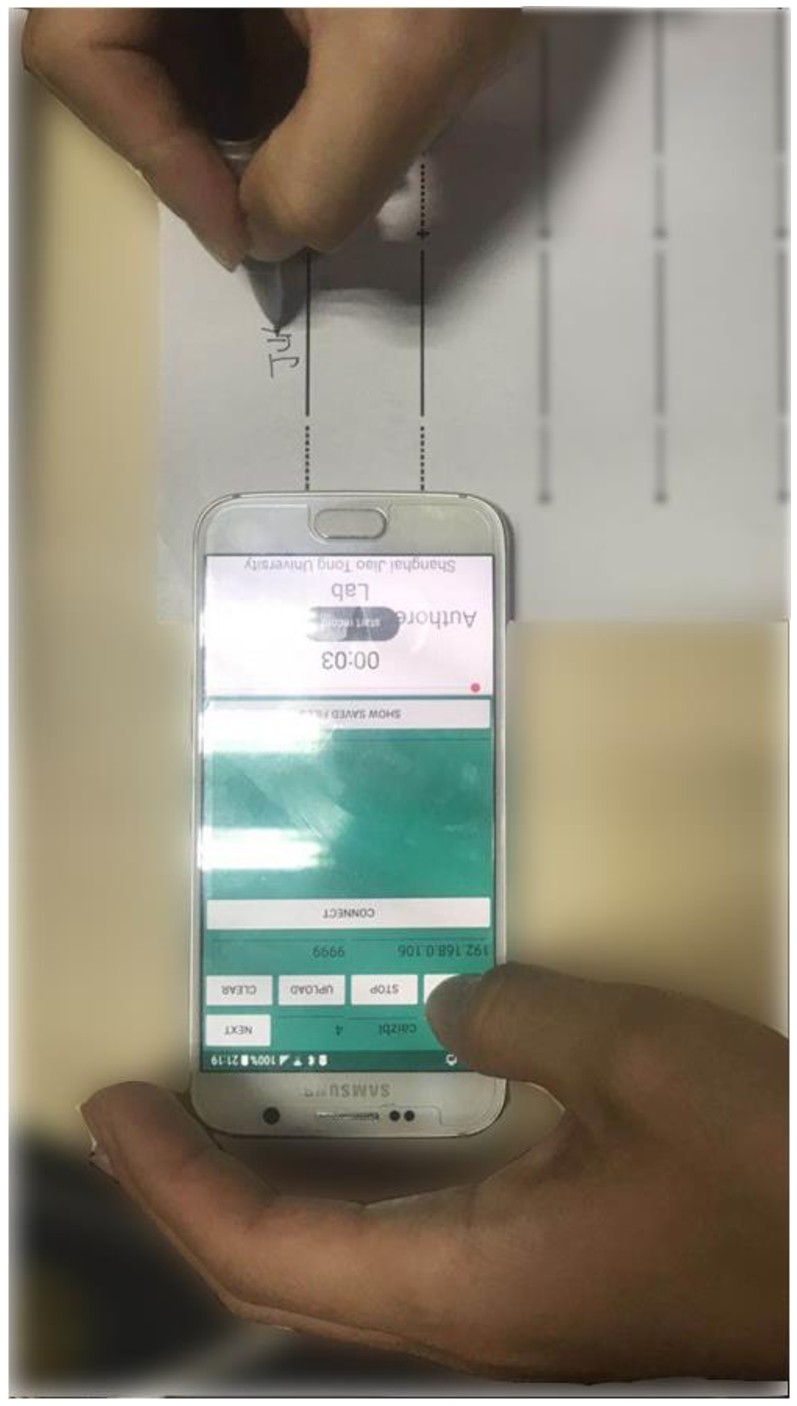
\includegraphics[width=\textwidth]{figure/app-data-collection.pdf}
    \bicaption
    {数据采集}
    {Data collection}
    \label{fig:data-collection}
   \end{minipage}
\end{figure}

1)右手握住笔,做好准备在写线段上开始写的姿势;

2)使用左手点击\textit{start}按钮;

3)根据手机界面上的时间显示,在1秒钟之后开始写;

4)在书写动作结束之后,使用左手点击\textit{stop}按钮。注意,每写完一个签名,手机界面上的计数器会自增一次,计数器上的数字组成了保存声波数据文件的文件名前缀。

14名研究生志愿者被邀请参加两阶段的签名实验,14位志愿者包含3名女生和11名男生,所有的志愿者习惯使用右手写字。两阶段的签名实验过程如下:

(1)在第一阶段,每个志愿者被邀请书写他/她的签名。每个志愿者会写112个签名,大概耗费30分钟。

(2)在第二阶段,随机地打乱志愿者的名单以获得一个循环队列。向志愿者展示循环队列中在他/她之后的五个志愿者的签名记录。为了成为一个熟练的模仿者,志愿者必须照着被模仿者的签名记录练习模仿签名,以致于模仿的签名和被模仿者的足够相似,然后为每个选中的被模仿者提供12个模仿签名。

总之,每个志愿者有112个真实签名和60个熟练仿造签名。

两星期后又另外邀请了22位本科生志愿者帮助做签名实验,由4名女生和18名男生组成,他们都是习惯使用右手写字,限于每位学生只有15分钟的实验时间,每位本科生被要求写32个真实签名和16个熟练模仿签名,后18位学生志愿者,每人需要模仿他/她前面4个同学的签名,为每个被模仿者提供4个熟练模仿签名,因此对于前18个志愿者,他们每人有32个真实签名和16个熟练模仿签名。最后,没有使用后4位同学提供的真实签名。由于每次实验的时间限制,这个本科生的数据集比研究生的数据集质量差,但是这个数据集可以用作交叉用户可用性测试。

\section{硬件补偿评估实验}
为了评估启发式方法的硬件补偿方案,本研究生成了两个WAV格式的音频文件:一个使用了硬件补偿,另外一个没有使用硬件补偿,每个音频文件以48 kHz的频率播放6秒钟。在每种情况中,截取第3秒记录的声波数据,对这些数据做FFT,获得48000个输出系数,考虑在8个频率上的FFT系数幅度。如图~\ref{fig:fft-wo-compensation}所示,当没有使用硬件补偿方法时,最小值、最大值、极差和标准差分别是77.8、323.5、245.7和76.4。相反地,如图~\ref{fig:fft-compensation}所示,当使用硬件补偿方法时,最小值、最大值、极差和标准差分别是137.2、164.4、27.1和8.5。很明显,硬件补偿方法大大减少了极差和标准差。进一步,由于过小的幅度导致过小的信噪比,因此该硬件补偿方案通过增加最小值的幅度还可以避免一种情况:在任何一个频率上的信噪比都不至于过小。
\begin{figure}[!htp]
  \centering
  \begin{minipage}[t]{0.49\textwidth}
    \centering
    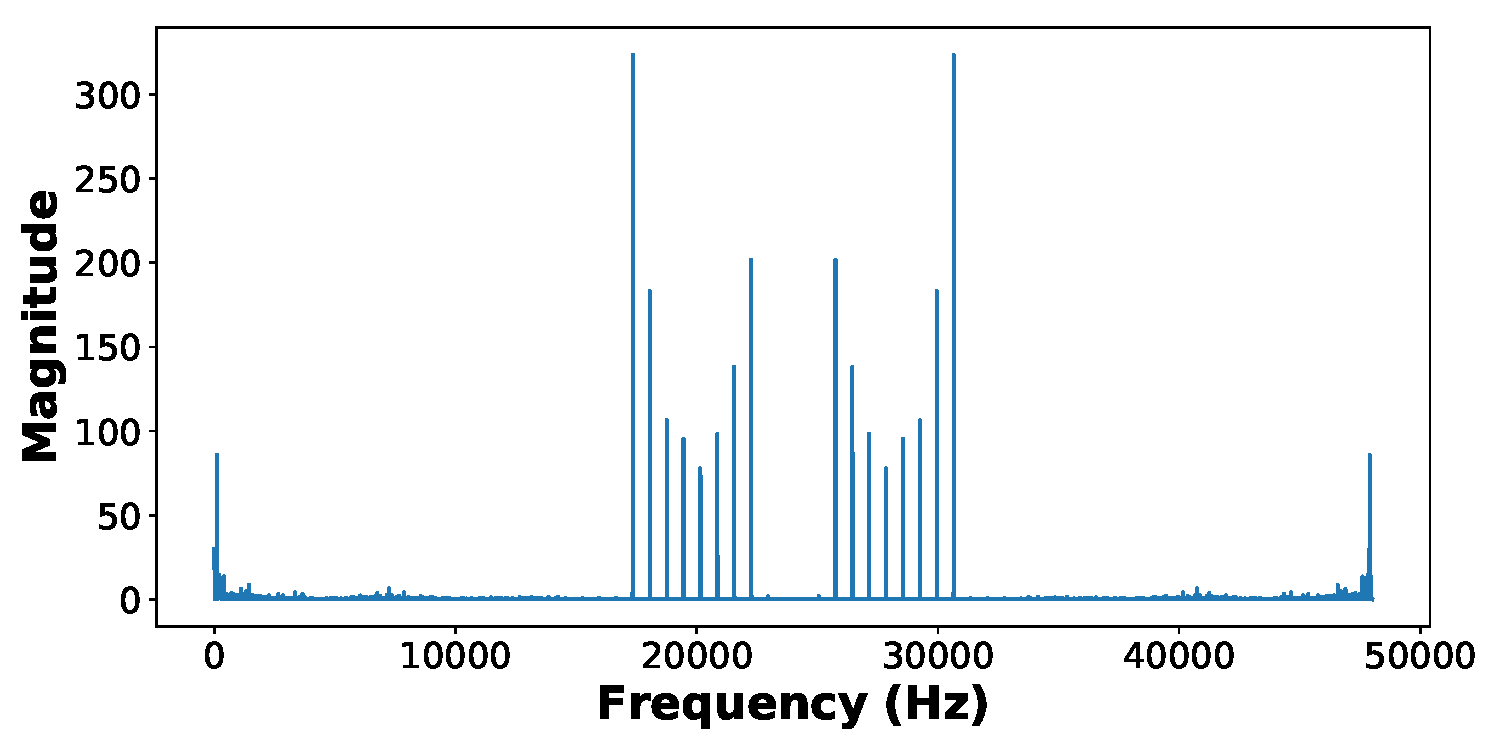
\includegraphics[width=\textwidth]{figure/nocompensation.pdf}
      \bicaption{没有硬件补偿时的FFT系数幅度}
      {FFT coefficient magnitudes w/o compensation}
        \label{fig:fft-wo-compensation}
  \end{minipage}
  \centering
  \begin{minipage}[t]{0.49\textwidth}
    \centering
    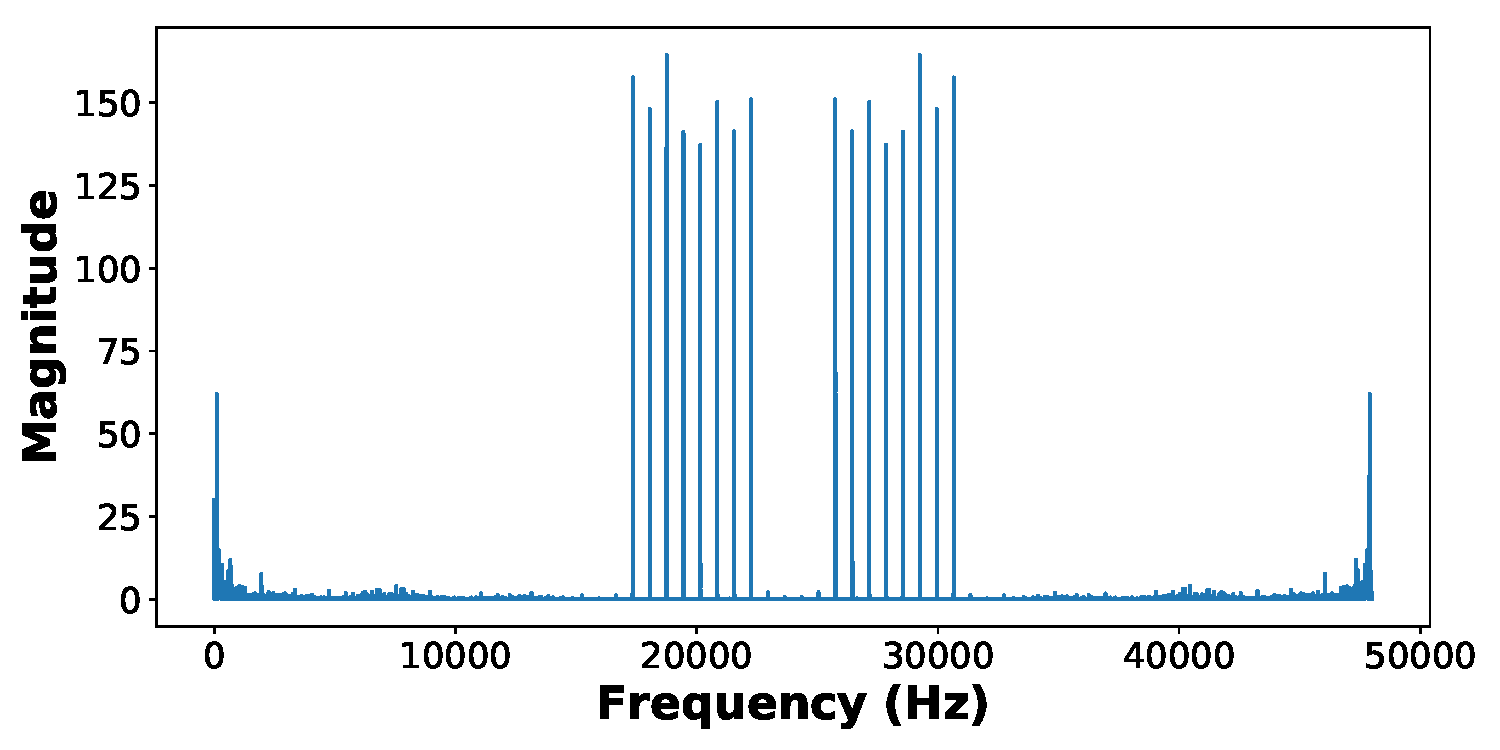
\includegraphics[width=\textwidth]{figure/compensation.pdf}
    \bicaption
    {有硬件补偿时的FFT系数幅度}
    {Smartphone setting}
    \label{fig:fft-compensation}
   \end{minipage}
\end{figure}

\section{精度评估实验}
\label{sec:accuracy-experiment}

与相关研究~\cite{fischer2015robust,levy2018handwritten}类似,本研究使用两个度量指标衡量验证准确度:ROC曲线下方的面积AUC和等错误率EER。EER是ROC曲线中FAR(false acceptance rate)和FRR(false rejection rate)相等的点,一个出色的手写签名认证系统应该具备较高的AUC和较低的EER。在本节评估中,使用研究生数据集进行分析和评估,展示在熟练仿冒者、随机仿冒者和两者结合这三种情况下的两个度量指标的值。给定一个志愿者,通过在其余志愿者的真实签名集中随机挑选4个签名,来组成该志愿者的随机仿造签名的集合,所以每个志愿者具有112个真实签名,60个熟练仿造签名和65个随机仿造签名。

打乱每个研究生的真实签名,前20个真实签名被用作参考签名,它们被用于产生参考矩阵$S_{reference}$(\S\ref{sec:feature-distance-matrix}),接下来的90个签名被用作查询签名,和参考矩阵相结合,用于产生距离矩阵。随机地从熟练模仿签名中挑选45个,从随机模仿签名中挑选45个,这样每名研究生志愿者总共有180个签名,包括:90个真实签名、45个熟练模仿签名和45个随机模仿签名,将总共拥有$180\times 14=2520$个带标签记录。再次将这些记录打乱,将它们分为:训练集和测试集两个部分,训练集有1764条带标签记录,占总记录数的70\%,测试集有756条带标签记录,占总记录数的30\%。为了绘制ROC曲线,通过改变CNN模型输出值(0到1)的阈值,获得一系列的TPR(true positive rate)和相对应的FPR(false positive rate)。给定一个查询签名,如果CNN模型的预测值大于选中的阈值,它将被判别为真实签名,否则将被判定为仿造签名。图~\ref{fig:roc-forgers}展示
\begin{figure}[!htp]
  \centering
  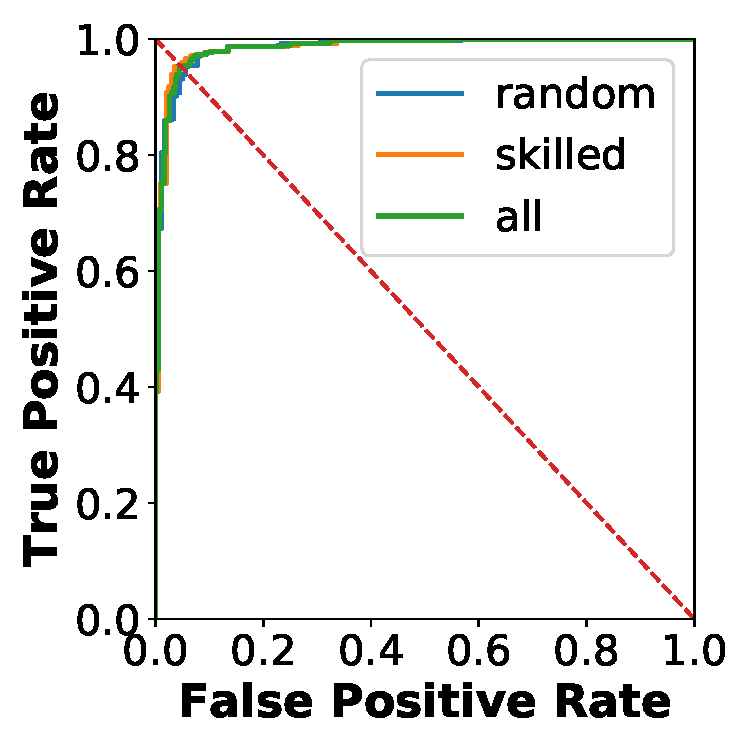
\includegraphics[width=0.4\textwidth]{figure/mimic-random-total-ROC-curves.pdf}
  \bicaption{三种仿造类型的ROC曲线}
      {ROC curves for the three types of forgers}
  \label{fig:roc-forgers}
\end{figure}
了三条ROC曲线,包括:熟练仿造签名情况下的ROC曲线、随机仿造签名情况下的ROC曲线和两种都有的情况下的ROC曲线。为了计算三种情况下的AUC值,计算三条ROC曲线下方的面积,为了获得三种情况下的EER值,在单元正方形中绘制一条主对角线,从该对角线与ROC曲线的交点可以获得EER值。

将以上过程重复了20次,从而可以求得AUC和EER值的平均值。如图~\ref{fig:mean-auc-forgers}所示,
\begin{figure}[!htp]
  \centering
  \begin{minipage}[t]{0.49\textwidth}
    \centering
    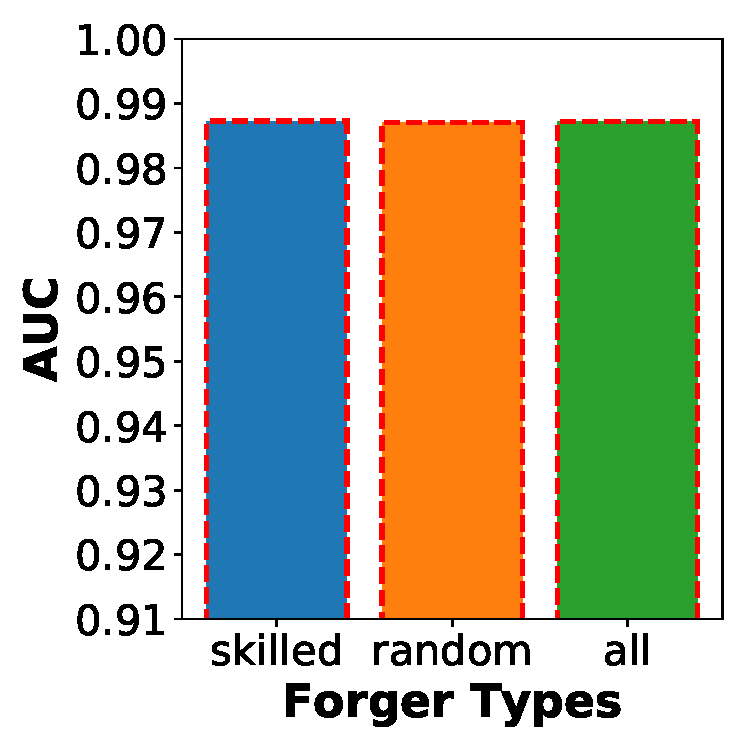
\includegraphics[width=\textwidth]{figure/auc-bars.pdf}
      \bicaption{三种仿造类型的平均AUC值}
      {Mean AUCs for the three types of forgers}
        \label{fig:mean-auc-forgers}
  \end{minipage}
  \centering
  \begin{minipage}[t]{0.49\textwidth}
    \centering
    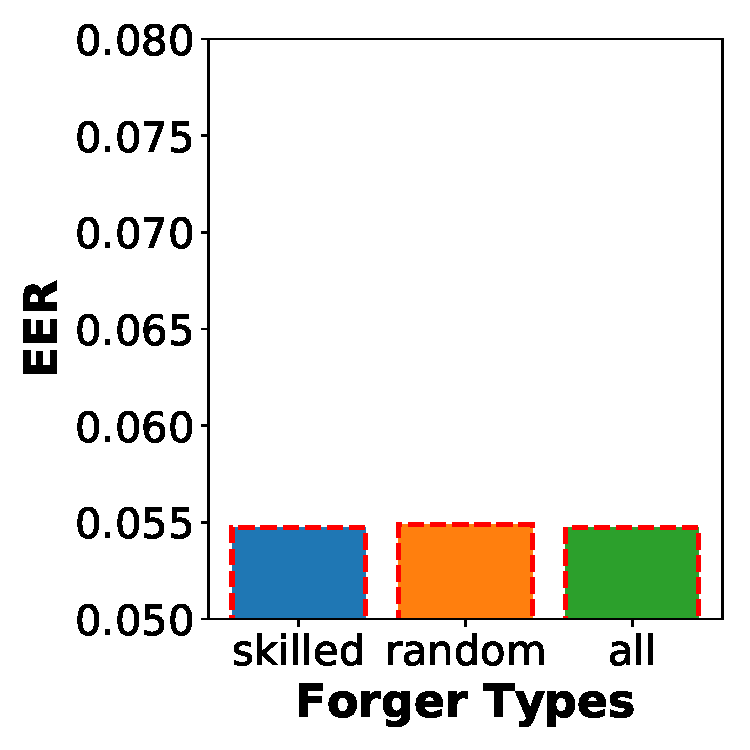
\includegraphics[width=\textwidth]{figure/eer-bars.pdf}
    \bicaption
    {三种仿造类型的平均EER值}
    {Mean ERRs for the three types of forgers}
    \label{fig:mean-eer-forgers}
   \end{minipage}
\end{figure}
在随机仿冒的情况下AUC=0.987,在熟练仿冒的情况下AUC=0.987,在两者结合的情况下AUC=0.987。如图~\ref{fig:mean-eer-forgers}所示,在随机仿冒的情况下EER=0.055,在熟练仿冒的情况下EER=0.055,在两者结合的情况下EER=0.055。通常地,因为熟练仿造的签名往往与真实签名在形状上非常相似,所以当使用扫描图像识别熟练仿造签名的离线签名认证系统会遭受巨大挑战,然而ASSV在熟练仿造签名识别中表现出了良好的性能。

\section{交叉用户可用性}

关于交叉用户可用性的实验中使用的CNN模型,使用研究生志愿者的数据集作为训练集,使用本科生志愿者的数据集作为测试集。这种类型的实验经常被现有的研究工作所忽略,这些研究的测试集和训练集中的用户有重合。本研究的系统模型是一个用户独立的模型,当有新用户注册的时候,可以不需要额外的高开销的训练过程,所以进行一个交互用户可用性测试是非常有必要的。在实验中采用10个参考签名通过重复切分数据集和训练操作,得到20个模型,然后建立测试数据集,对于每个测试用户,随机挑选10+20个真实签名(10个参考签名和20个真实签名),10个熟练仿造签名,10个随机仿造签名(挑选五个其他用户,每用户提供2个真实签名),最终拥有$22\times (20+10+10)=880$个距离矩阵用于测试。重复以上生成距离矩阵集合的过程10次,获得10个不同距离矩阵集合。

接着实施评估,$20\times 10=200$个AUC和EER对被获得而用于计算平均AUC和EER对,如表~\ref{table:cross-eer}和表~\ref{table:cross-auc}所示,
\begin{table}[ht]
  \centering
    \bicaption{交叉用户可用性 - EER}
    {Cross-user usability - EER}
    \label{table:cross-eer}
    \begin{tabular}{c c c c}
      \hline\hline 
      Model & Random(\%) & Skilled(\%) & All(\%) \\ 
      \hline 
      No-cross-user & 6.1 & 5.8 & 5.8 \\
      Cross-user & 14.1 & 19.9 & 17.1 \\
      Retrained & 4.4 & 9.4 & 7.9 \\
      \hline 
    \end{tabular}
\end{table}
\begin{table}[ht]
  \centering
  \bicaption{交叉用户可用性 - AUC}
  {Crooss-user usability - AUC} 
  \label{table:cross-auc} 
  \begin{tabular}{c c c c} 
    \hline\hline 
    Model & Random(\%) & Skilled(\%) & All(\%) \\ 
    \hline 
    No-cross-user & 98.3 & 98.5 & 98.4 \\
    Cross-user & 92.8 & 88.3 & 90.5 \\
    Retrained & 99.0 & 97.6 & 98.2 \\
    \hline 
  \end{tabular}
\end{table}
相比于非交叉用户评估,交叉用户试验的性能有所下降,但是系统仍然保持不错的交叉用户可用性。

将测试模型用作一个预训练模型,测试集中20\%的数据用于再次训练模型从而获得一个新的模型,这个模型使用剩下的80\%的数据进行测试,结果发现性能得到了很大的提升:第一种情况中,EER达到4.4\%,AUC达到99.0\%;第二种情况中,EER达到9.4\%,AUC达到97.6\%;第三种情况中,EER达到7.9\%,AUC达到98.2\%。

\section{鲁棒性评估实验}
\label{sec:robustness-experiment}
为了测试系统的鲁棒性,本研究做了三种实验:不同环境下的实验、不同距离下的实验和不同日期下的实验,邀请了4位志愿者参与鲁棒性实验,包括2位男性和2位女性。在每种实验的每种情况下,每位志愿者被要求写下20个他/她的签名。在同一个鲁棒性实验中的所有情况中,选择其中一个情况中所得的签名用作参考签名,人工地选择那个用作参考签名的情况。实际上,一个适应算法可以在未来被提出用于为每个用户选择合适的签名,这个超出了本文的研究范围。记录分类器的每个输出(0-1),对于每个查询情况输出值的中位数规整为0-100的度量值,越高的度量值意味着查询签名和参考签名之间的相似度越高,进一步意味着系统更具鲁棒性。三种鲁棒性实验的具体情况如下:

\textbf{(1)不同环境}:每名志愿者被要求在三个不同的环境下进行签名,这三个环境包括:安静的环境,有播放音乐的环境,有人在旁边行走的环境。在安静的环境中,没有人在房间内说话,也没有人走路;在有播放音乐的环境中,另外一个智能手机放在是实验智能手机的旁边播放音乐;在有人在旁边行走的环境中,有人在实验者签名的时候在其旁边行走。

\textbf{(2)不同距离}:每个志愿者被要求在改变智能手机到签名线的距离时,进行签名。这些距离包括:3cm, 6cm,9cm。

\textbf{(3)不同日期}:每个志愿者被要求在不同的日期下进行签名,总共有3个不同的日期。


表~\ref{table:system-robustness}显示
\begin{table}[ht]
  \centering
  \bicaption[系统鲁棒性]
  {系统鲁棒性 - \textbf{RS} 意思是 \textit{reference signatures}(参考签名)}
  {System robustness - \textbf{RS} means \textit{reference signatures}}
  \label{table:system-robustness}
  \begin{tabular}{|c|ccc|ccc|ccc|}
    \hline
    \multirow{2}{*}{\textbf{Volunteer}} & \multicolumn{3}{|c|}{\textbf{Environment}} & \multicolumn{3}{|c|}{\textbf{Distance}} & \multicolumn{3}{|c|}{\textbf{Day}} \\
    \cline{2-10}
     & \textit{Quiet} & \textit{Music} & \textit{Walk} & \textit{3 cm} &  \textit{6 cm} & \textit{9 cm} & \textit{Day 1} & \textit{Day 2} & \textit{Day 3}\\
    \hline
    No. 1 & RS   & 93.3 & 86.1  & \textbf{4.8} & 91.4 & RS &  RS & \textbf{67.1} & 93.4  \\  
    \hline
    No. 2 & RS & 81.2 & 93.3  & \textbf{53.3} & 93.6 & RS & RS & 94.0 & 95.4 \\
    \hline
    No. 3 & RS & 94.4 & 97.3  & \textbf{57.3} & 89.8 & RS & RS &  94.4 & 96.7 \\
    \hline
    No. 4 & RS & 83.2 & 84.8  & \textbf{4.4} & 84.9 & RS & RS &  84.6 & 90.1 \\
    \hline 
  \end{tabular}
\end{table}
了鲁棒性实验结果。在改变环境或日期的情况下,本文中的系统保持了鲁棒性。然而,当将智能手机和签名线之间距离设置为9cm的情况下所得的签名作为参考签名,发现在3cm的情况下所得的签名作为查询签名时效果较差,而在6cm的情况下所得的签名作为查询签名时的效果还算可以,由此可知,当查询签名和参考签名相距为6cm时,系统性能变差。因此,建议查询签名和参考签名的距离最好控制在3cm以内。


\section{微基准测试}
ASSV在通过改变一些内部参数的情况下被评估,这些参数包括:参考签名的数量,CNN卷积核的数量,训练集大小,DCT系数数量,声波频率数量和分类器类型。

\subsection{参考签名数量}
为了评估在签名认证时,参考签名数量对AUC和EER结果的影响,选择在参考签名数量在1到22时测试系统。对于每个选择的参考签名数量,通过重复实验(参考~\S\ref{sec:accuracy-experiment})来得到平均的AUC和EER。图~\ref{fig:rcount-auc-lines}
\begin{figure}[!htp]
  \centering
  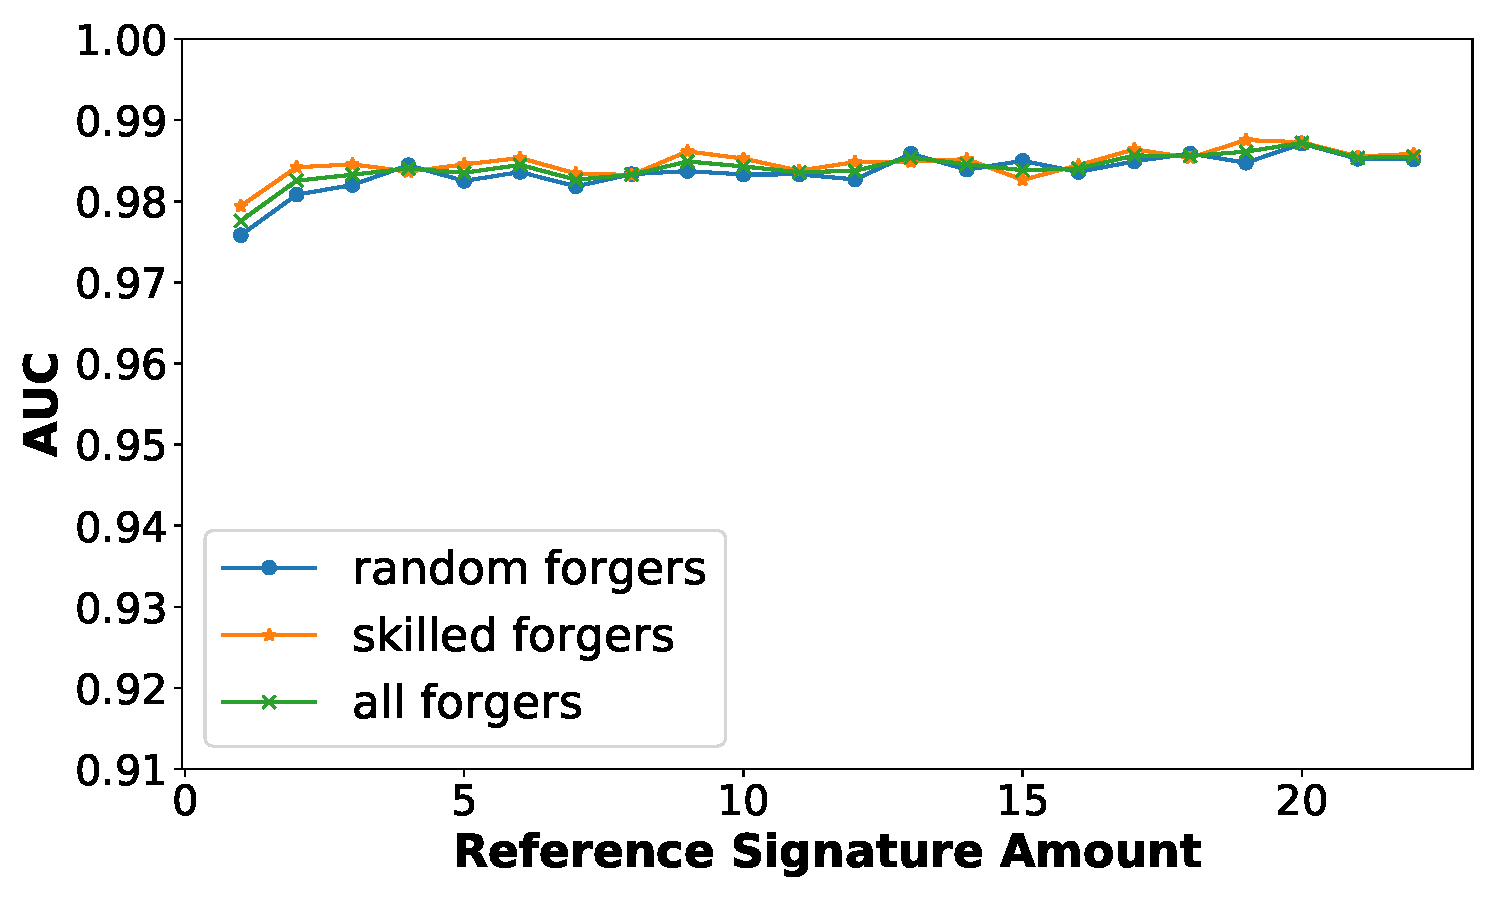
\includegraphics[width=0.6\textwidth]{figure/rcount-auc-lines.pdf}
  \bicaption{参考标签数量影响 - AUC}
      {Reference amount effect - AUC}
  \label{fig:rcount-auc-lines}
\end{figure}
和图~\ref{fig:rcount-eer-lines}显示
\begin{figure}[!htp]
  \centering
  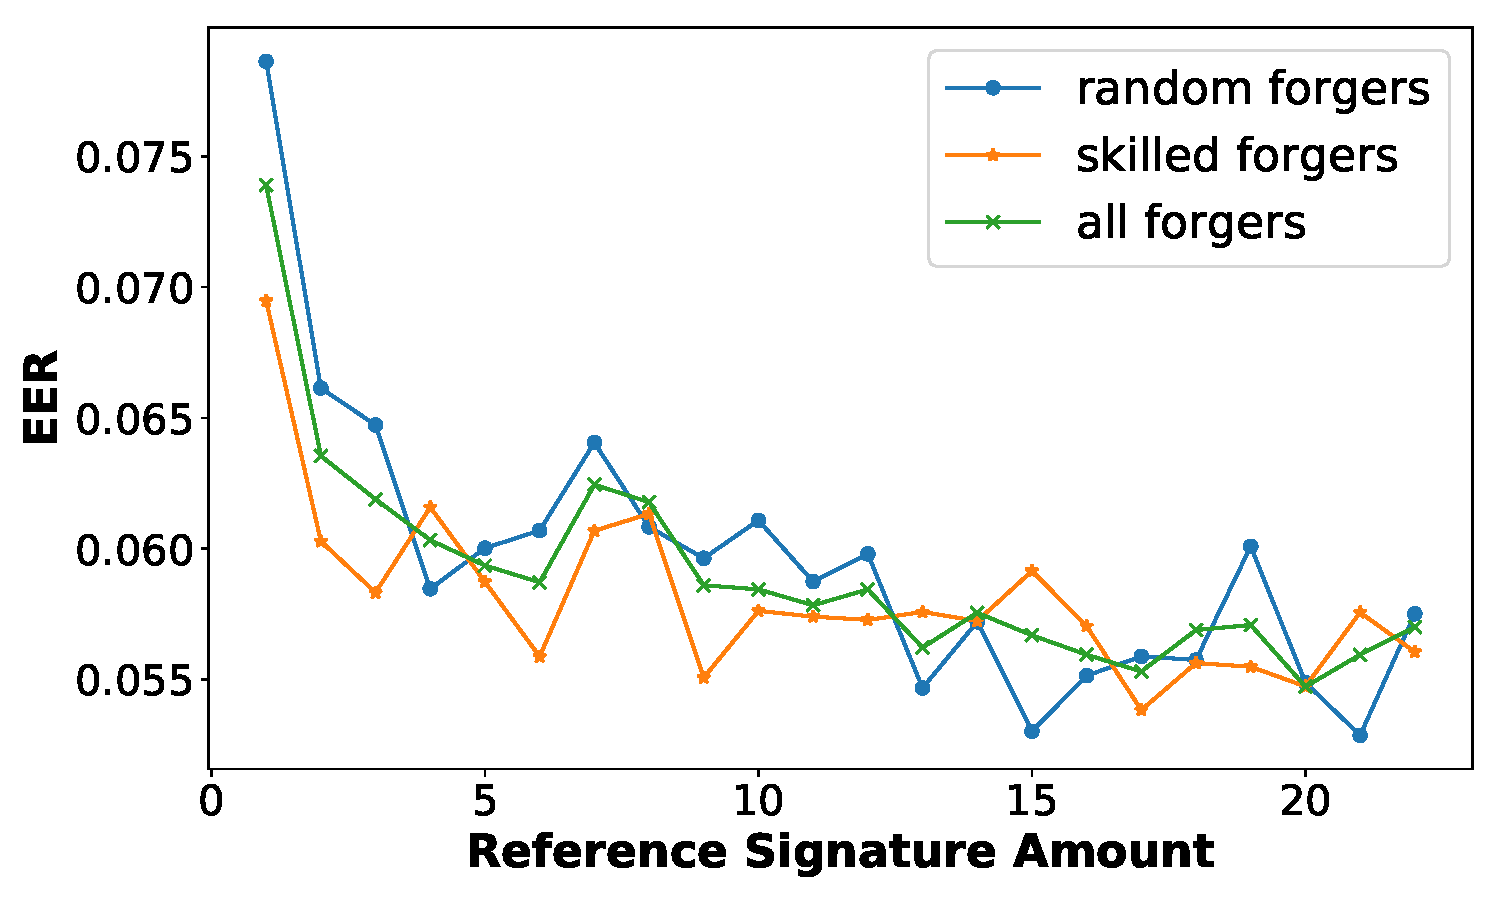
\includegraphics[width=0.6\textwidth]{figure/rcount-eer-lines.pdf}
  \bicaption{参考标签数量影响 - EER}
      {Reference amount effect - EER}
  \label{fig:rcount-eer-lines}
\end{figure}
了改变参考签名数量的试验结果。总体上,当参考签名数量增加,系统性能变好。当仅仅使用一个参考签名时,AUC=0.978和EER=0.074,当使用6个参考签名时,AUC=0.984 和 EER=0.059,可见当参考签名从1个增加到6个时,系统性能快速改善。在那之后,随着参考签名数量的增加,系统改善幅度变化不明显,意味着:通过增加参考签名所得到的益处开始收敛。所以本系统只需要很少的参考签名数量,就能达到良好的性能,好处是在用户注册阶段,新用户只需要花费较少的时间去写参考签名,这样使得本文的系统更加用户友好。


\subsection{CNN卷积核的数量}
选择20作为参考签名的数量,将CNN卷积核数目设置为8、16、32、64、128和256,在不同的卷积核数量情况下测试系统性能。图~\ref{fig:filter-number-effect}显示
\begin{figure}[!htp]
  \centering
  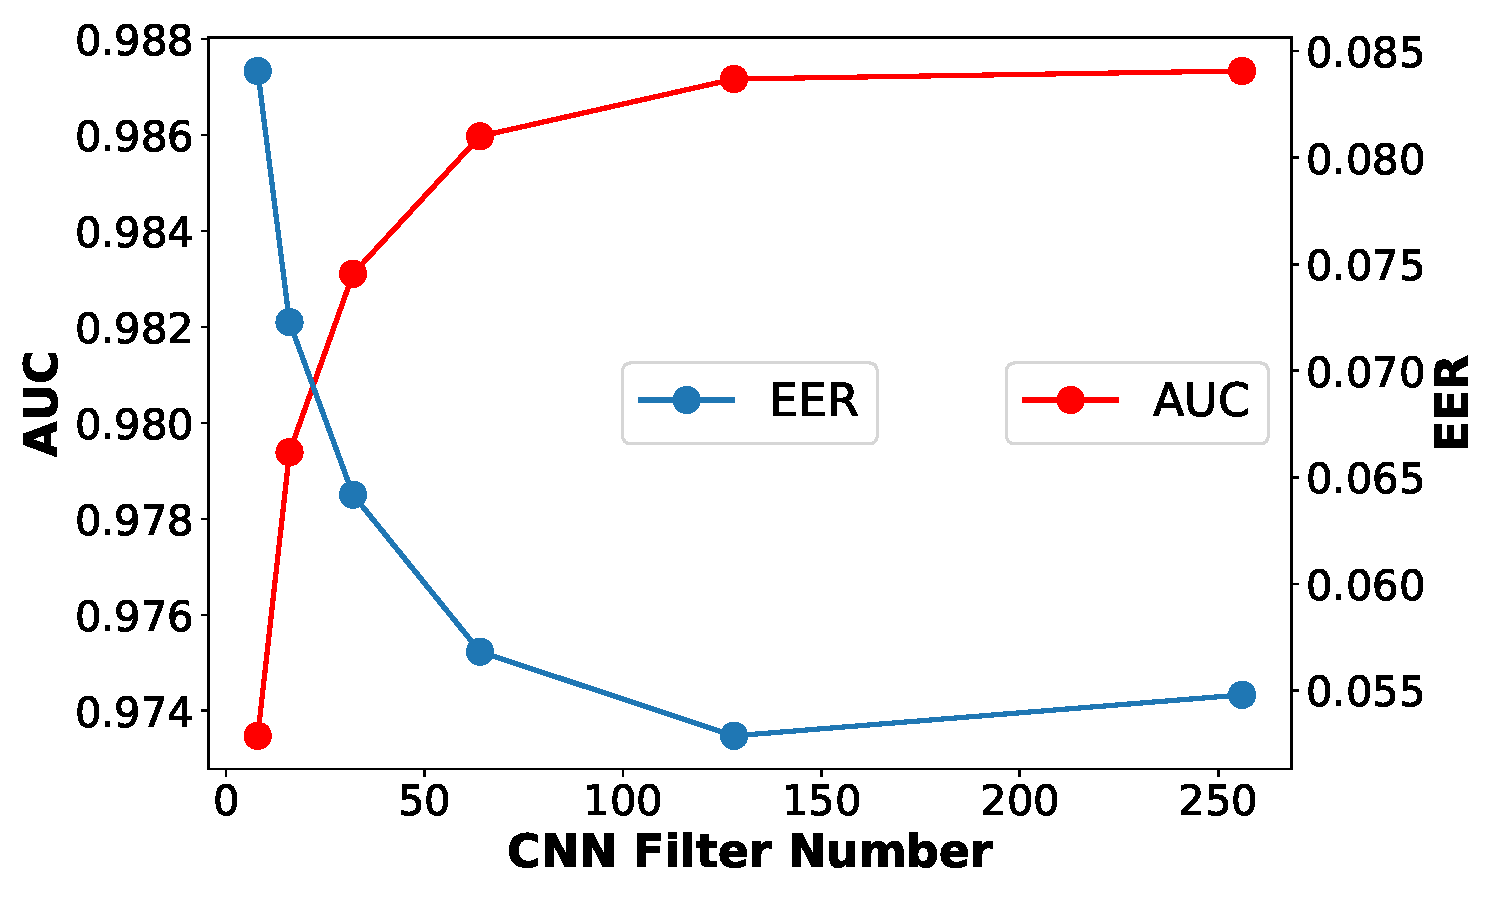
\includegraphics[width=0.5\textwidth]{figure/filter_number_auc_eer.pdf}
  \bicaption{CNN卷积核数量的影响}
      {CNN filter number effect }
  \label{fig:filter-number-effect}
\end{figure}
了在第三种情况下(\textit{all forgers})的AUC和EER的结果:当卷积核数量从8增加到128时,系统性能变得更好;当卷积核数量为128时,系统性能达到最佳:AUC=0.987 和 EER=0.053;即使当卷积核数量为最小的8时,结果仍然可以达到AUC=0.973 和 EER=0.084,显示出了特征提取的成功。 

\subsection{训练集大小}
选择20作为参考签名的数量,128作为卷积核数量。为了评估训练集大小对试验结果的影响,保持测试集的大小不变,将训练集的大小改变成100,300,...,1700。如图~\ref{fig:train-size-effect}所示,
\begin{figure}[!htp]
  \centering
  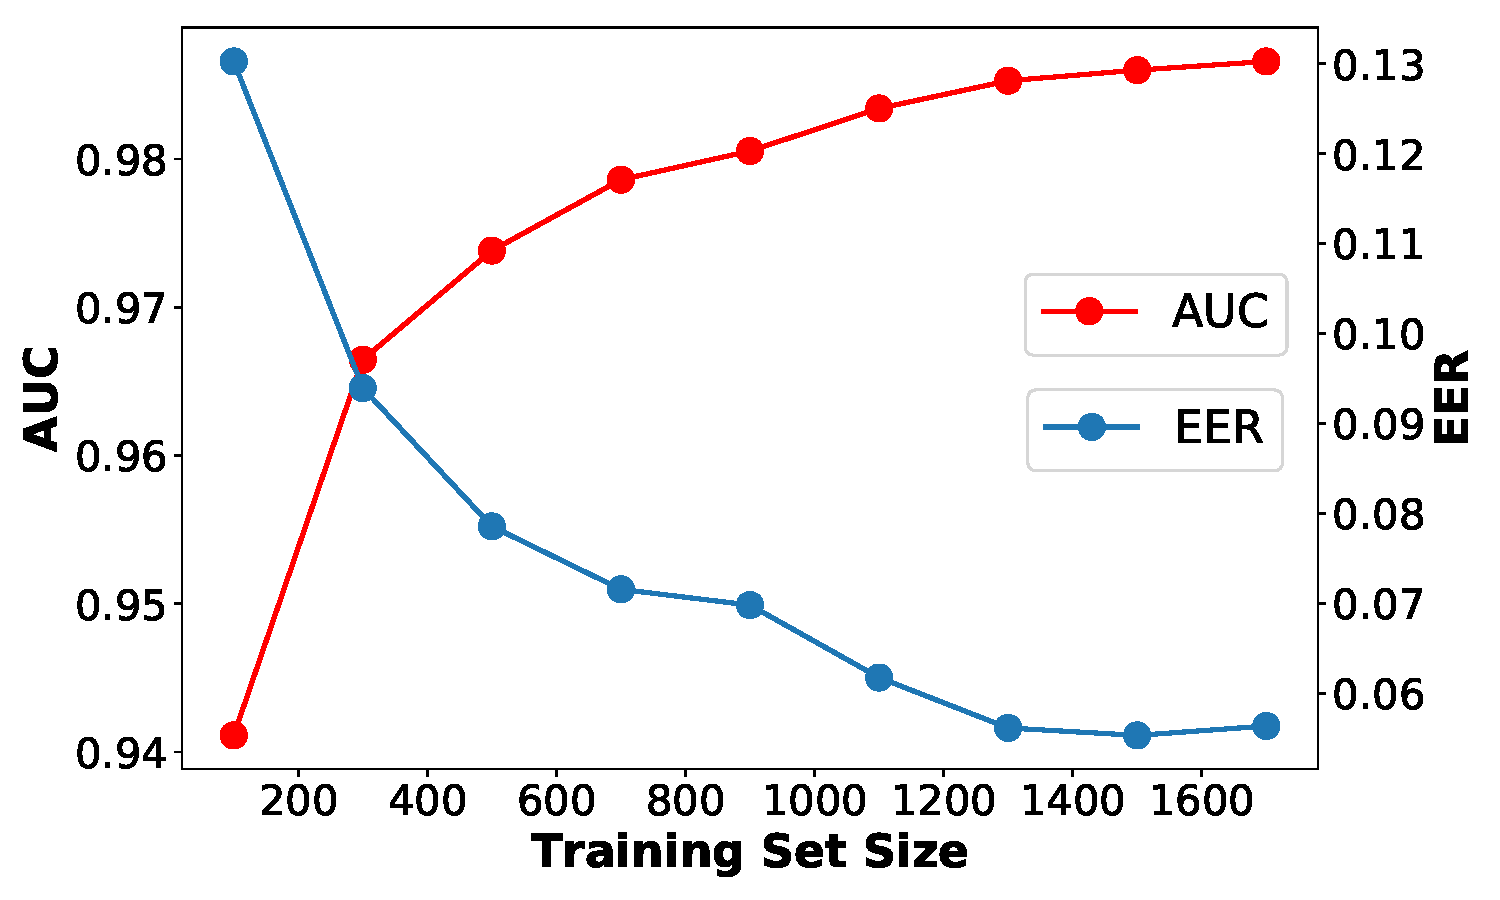
\includegraphics[width=0.5\textwidth]{figure/train_size_auc_eer.pdf}
  \bicaption{训练集大小的影响}
      {Train set size effect }
  \label{fig:train-size-effect}
\end{figure}
当训练集大小从100增加到1700时,AUC从0.814增加到0.980,EER从0.263增加到0.071。就如预期的那样,当训练集大小增加到一定程度后,AUC和EER的曲线开始收敛。

\subsection{DCT系数数量}
选择20作为参考签名的数量,为了评估DCT系数数量对实验结果的影响,将DCT系数数量设置为8、9、10、15、20、25、30、35和40。对前面的几个DCT系数数量设置间隔较小,实现较为精细的评估。在三种情况下测试DCT系数的数量的影响:第一种情况下,只有相位变化的速度信息被使用;第二种情况下,只有相位变化的加速度信息被使用;第三种情况下,相位变化的速度信息和加速度信息都被使用。假设$C$表示被设置的DCT系数数量,所以在前两种情况下,距离矩阵的形状为($C$, 8, 3),而在第三种情况中,距离矩阵的形状为($C$, 8, 6)。图~\ref{fig:dct-total-auc}和图~\ref{fig:dct-total-eer}显示了评估结果,
\begin{figure}[!htp]
  \centering
  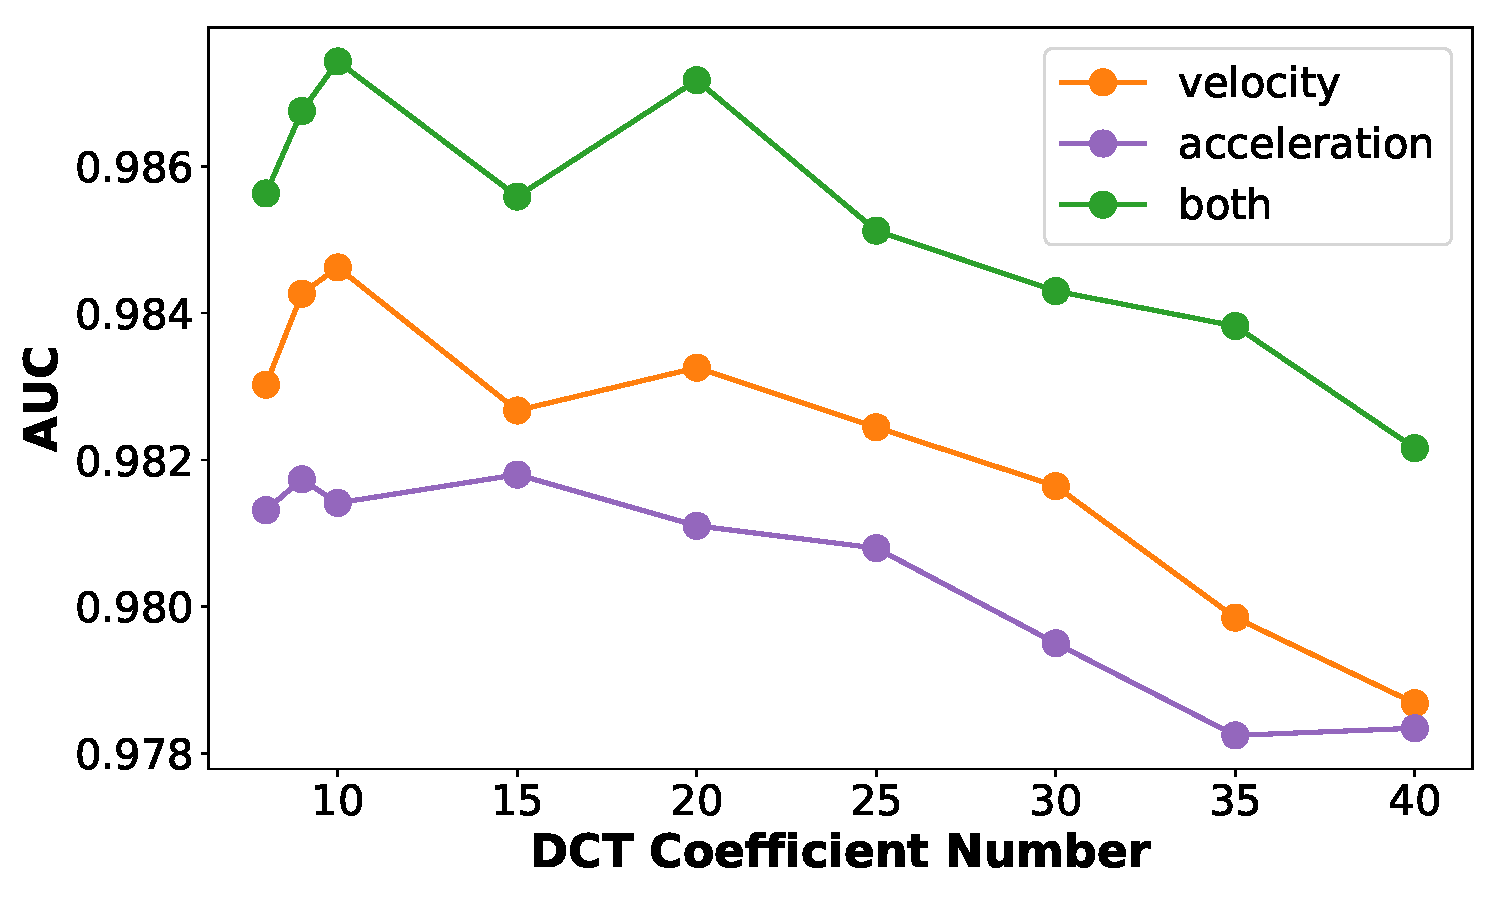
\includegraphics[width=0.5\textwidth]{figure/dct_total_auc.pdf}
  \bicaption{DCT系数数量 - AUC}
      {DCT coefficient number - AUC}
  \label{fig:dct-total-auc}
\end{figure}
\begin{figure}[!htp]
  \centering
  \includegraphics[width=0.5\textwidth]{figure/dct_total_eer.pdf}
  \bicaption{DCT系数数量 - EER}
      {DCT coefficient number - EER}
  \label{fig:dct-total-eer}
\end{figure}
当DCT系数数量是从8到40的时候,只使用相位变化的速度信息的系统性能优于只使用加速度信息的系统,总体上相位变化的速度信息和加速度信息的结合可以提升系统性能。接着,将注意力转移到第三种情况中,如图~\ref{fig:dct-total-auc}所示,当时DCT系数数量为10时,系统的性能达到最佳,当DCT系数继续增加的时候,由于噪音的增加,系统性能开始变差。

\subsection{声波频率数量}
选择20作为参考签名的数量。为了评估频率数量对试验结果的影响,将频率数量设置为$FN=3, 4,..., 8$。所以,距离矩阵的形状为$(10, FN, 6)$。由于\textit{max pooling}的降维效果,当频率数量小于8的时候,两层卷积池化层将无法工作。因此,为了能够顺利训练和测试模型,在原有的CNN模型基础上减去了一层卷积池化层,使用修改后的模型。图~\ref{fig:frequency-number}报告
\begin{figure}[!htp]
  \centering
  \includegraphics[width=0.5\textwidth]{figure/multi_frequency_auc_eer.pdf}
  \bicaption{频率数量的影响}
      {Frequency number effect}
  \label{fig:frequency-number}
\end{figure}
了结果。当频率从3增加到8的时候,AUC从0.977增加到0.984,EER从0.074减少到0.063。所以,多频率的使用可以使得ASSV更加鲁棒和准确。

\subsection{分类器类型}

选择20作为参考签名的数量,为了比较本研究的CNN模型和传统分类器的效果,将CCN模型替换为传统的分类器,比如随机森林、支持向量机或者朴素贝叶斯作为二分类器。如表~\ref{table:classifier-auc}和表~\ref{table:classifier-eer}所示,
\begin{table}[ht]
  \centering
  \bicaption
  {分类器 - AUC}
  {Classifier - AUC} 
  \label{table:classifier-auc} 
  \begin{tabular}{c c c c} 
      \hline\hline 
      Classifier & Random(\%) & Skilled(\%) & All(\%) \\ 
      \hline 
      Naive Bayes & 86.1 & 83.5 & 84.8 \\
      SVM & 92.5 & 96.3 & 94.5 \\
      Random Forest & 93.8 & 93.5 & 93.6 \\
       \textbf{CNN} &  \textbf{98.3} &  \textbf{98.5} &  \textbf{98.4} \\
      \hline 
  \end{tabular}
\end{table}
\begin{table}[ht]
  \centering
    \bicaption
    {分类器 - EER}
    {Classifier - EER}
    \label{table:classifier-eer}
    \begin{tabular}{c c c c}
      \hline\hline 
      Classifier & Random(\%) & Skilled(\%) & All(\%) \\ 
      \hline 
      Naive Bayes & 14.6 & 18.2 & 16.3 \\
      SVM & 16.7 & 9.0 & 12.3 \\
      Random Forest & 7.2 & 7.5 & 7.3 \\
       \textbf{CNN} &  \textbf{6.1} &  \textbf{5.8} &  \textbf{5.8} \\
      \hline 
    \end{tabular}
\end{table}
随机森林模型也呈现了较好的结果(第三种情况中,AUC = 93.6和EER=7.3),但是本研究的CNN达到最佳性能(第三种情况中,AUC=98.4和EER=5.8)。

\section{经典系统对比实验}
选择一个离线手写签名认证系统~\cite{hafemann2017learning}来和ASSV进行比较。为了获得两个数据集,签名图像(尺寸: 483 $\times$ 312 $px$)被扫描和切割。根据~\cite{hafemann2017learning},使用第一个数据集作为\textit{development dataset},用于训练一个写者独立的人工神经网络,这个人工神经网络将被用于特征提取,第二个数据集将被用作\textit{exploitation dataset},每个用户的10个真实签名将被用于训练一个写者依赖的分类器。下载到源代码~\footnote{https://github.com/luizgh/sigver}用于评估,如表~\ref{table:the-state-the-art}所示,尽管~\cite{hafemann2017learning}达到了96.5\%的AUC和10.6\%的EER,使用了二次训练的模型的ASSV还是达到了最优性能。
\begin{table}[ht]
  \centering
    \bicaption
    {和经典系统的比较}
    {Comparison with the state-of-the-art}
    \label{table:the-state-the-art} 
    \begin{tabular}{c c c c} 
      \hline\hline 
      Model & AUC(\%) & EER(\%) \\ 
      \hline 
      The state-of-the-art & 96.5 & 10.6\\
      Cross-user & 90.5 & 17.1 \\
      \textbf{Retrained} & \textbf{98.2} & \textbf{7.8}\\
      \hline 
    \end{tabular}
\end{table}

\section{重放攻击实验}

在重放攻击实验中,2名自愿者被邀请参加写20个参考签名,并且在写的时候,放置了另外一个用于监听的智能手机在目标智能手机的旁边,在参考签名得到处理后,监听智能手机会对每个志愿者实施20次重放攻击。本文采用与~\S\ref{sec:robustness-experiment}中相似的度量指标,40个预测值的中位数是4.1,最大值在50到60之间。所以,如果将阈值设置为50,只有一次重放攻击能够成功;如果将阈值设置为60,那么所有重放攻击都是失败的。结果显示本文系统可以很好地处理这样的重放攻击。其中一个原因是,系统中所提取的特征与智能手机和手的相对位置具有很大的关联,除非监听器和目标智能手机在同一个位置,否则监听数据所得到的特征与真实值将有很大区别。另外,在攻击的时候,有两个智能手机在发射声波,所以接收的声波信号由两部分组成,这也会导致重放攻击的失败。

\section{本章小结}
本章对基于声波的手写签名认证方案进行了实验验证和评估。在线签名认证和离线签名认证已经被研究很长时间了,在这个领域有很多先进的方法被提出,它们大多数在已有的数据集上被评估和测试。本研究是第一次将声波信号应用到手写签名认证,之前的研究使用了多模信号,实现了较高精度,本研究仅仅使用声波信号便实现了较高精度。根据评估结果,ASSV已经达到满意的结果,并且只需要使用很少的参考签名。除了准确度外,还评估系统的交叉用户可用性、鲁棒性、重放攻击,实验显示出ASSV系统良好的可用性。

\chapter{基于声波的签名认证方案的系统设计与实现}

本章针首先分析基于声波的签名认证系统的用户需求,然后完成系统架构设计,接着实现基于声波的签名认证系统,最后进行一系列实验来评估系统的运行性能。

\section{系统需求分析}

本节将设计并实现基于声波的签名认证的原型系统——ASSV。本原型系统的主要目的是让用户可以在自己的手机上实时判别自己签名是否真实,及时给出反馈,主要针对的场景是需要使用手写签名进行身份认证的场景。系统的主要需求是:用户手写自己签名用于认证,系统给出签名真实性判别结果。通过进一步分析,将面向用户的主要功能展示于图~\ref{fig:use-case}的系统用例图中。
\begin{figure}[!htp]
  \centering
  \includegraphics[width=0.5\textwidth]{figure/use-case.png}
  \bicaption{系统用例图}
      {The use case diagram}
  \label{fig:use-case}
\end{figure}

面向用户的主要功能如下:

\textbf{(1)注册。}用户使用系统之前,需要写一定数量的参考签名完成注册,完成注册之后,才能使用认证功能。

\textbf{(2)认证。}用户在认证的时候,开始记录签名动作,完成签名,系统给出反馈,告诉用户这个签名的真实性。


\section{系统设计与实现}
\subsection{系统框架设计}

根据对基于声波的签名认证系统的需求分析,为保证原型系统具有良好的可扩展性和可维护性,本研究对原型系统采用分层架构。框架设计如图~\ref{fig:system-framework},
\begin{figure}[!htp]
  \centering
  \includegraphics[width=0.5\textwidth]{figure/prototype-architecture.pdf}
  \bicaption{系统架构设计}
      {The design of system framework}
  \label{fig:system-framework}
\end{figure}
系统从下到上分为三层:最下层是数据层,主要功能是负责扬声器和麦克风相关系统接口的调用和协调,播放预先生成的音频文件发射声波,接收声波数据,上传给上层;中间层是业务逻辑层,主要负责接收到原始声波数据之后的相关处理,包括:信号下转化、相位信息估计、特征提取和分类;最上层是表示层,主要是提供一个和用户的交互UI,包括应用程序的注册界面和认证界面,用户从界面发出命令给系统,相应结果也由界面展示。整个系统分为两部分:服务端和安卓端,服务端用Python实现,运行CNN预测模型,其余部分都在安卓端实现,通过socket实现安卓端和服务端的通信。 


\subsection{数据层}
数据层主要负责声波的发射和接收,由于需要与外设扬声器和麦克风通信,这部分需要调用相关的安卓系统接口。安卓版本为android 7,apk文件的最小sdk版本是21,目标和编译sdk版本都是27。

在发射声波部分,需要调用扬声器相关的API,android.media.MediaPlayer类来实现对预先生成音频文件的播放来发射声波。如代码~\ref{src:create-media-player}所示,

\begin{lstlisting}[language={Java}, caption={创建MediaPlayer对象 \label{src:create-media-player}}]
mediaPlayer = MediaPlayer.create(this, R.raw.sound)   //创建MediaPlayer对象
\end{lstlisting}
需要创建一个MediaPlayer对象,第一个参数是上下文Context对象,第二个参数是音频文件的资源编号。代码~\ref{src:start-play}展示
\begin{lstlisting}[language={Java}, caption={开始播放 \label{src:start-play}}]
mediaPlayer.seekTo(0) //到开始位置
mediaPlayer.start()  //开始播放
\end{lstlisting}
了开始播放的执行过程,代码~\ref{src:pause-play}展示
\begin{lstlisting}[language={Java}, caption={暂停播放\label{src:pause-play}} ]
mediaPlayer.pause()  //暂停播放
\end{lstlisting}
了暂停播放的执行过程。在操作过程中,满足MediaPlayer的生命周期~\footnote{https://developer.android.com/reference/android/media/MediaPlayer},防止出错。

在接收声波部分,需要调用麦克风相关的API。使用android.media.AudioRecord类来实现声波的接收。如代码~\ref{src:create-audio-record}所示,
\begin{lstlisting}[language={Java}, caption={创建AudioRecord对象 \label{src:create-audio-record}} ]
audioRecord = AudioRecord(
ConfigInfo.audioSource,    //MediaRecorder.AudioSource.MIC
ConfigInfo.sampleRateInHz, //48000
ConfigInfo.channelConfig,  //AudioFormat.CHANNEL\_IN\_MONO
ConfigInfo.audioFormat,   //AudioFormat.ENCODING\_PCM\_FLOAT
ConfigInfo.bufferSize    // 48000*2*2
)
\end{lstlisting}


需要创建AudioRecord对象,它的startRecord和stop方法用于开始和停止声波数据的记录。麦克风产生的是流式数据,需要通过循环读来获取数据,如代码~\ref{src:read-data-stream}所示,将读到的数据写到一个输出流中。

\begin{lstlisting}[language={Java}, caption={读取数据流 \label{src:read-data-stream}} ]
fun writeData(outputStream: OutputStream) {
    val buffer: ByteBuffer = ByteBuffer.allocateDirect(ConfigInfo.bufferSize!! / 3) //创建Direct内存缓存区
    val byteArray: ByteArray = ByteArray(ConfigInfo.bufferSize!! / 3)   //创建缓存数组
    var len: Int = 0
    try {
        while (audioRecord!!.recordingState != AudioRecord.RECORDSTATE_RECORDING) {
        }
        do {
            len = audioRecord!!.read(buffer, buffer.capacity())   //循环读取数据流
            buffer.rewind()
            if (len > 0) {
                buffer.get(byteArray, 0, len)
                buffer.clear()
                outputStream.write(byteArray, 0, len)  //写入一个输出流中
            }
        } while (len > 0 || audioRecord!!.recordingState == AudioRecord.RECORDSTATE_RECORDING)
    } finally {
        outputStream.flush()
        outputStream.close()
    }
}
\end{lstlisting}


\subsection{业务逻辑层}
业务逻辑层拥有一条与数据层中的输出流通过管道相连的输入流,可以处理原始的声波数据,处理步骤包括:信号下转化、相位信息估计、特征提取和分类。当用户执行注册操作的时候,不需要分类步骤。安卓端业务逻辑部分使用Java实现,打包成Jar包,引入到安卓项目中;服务端的分类器使用Python实现;两者间,将数据使用Json序列化后,利用Socket进行TCP通信。

信号下转化,采用在线处理的方式,每获得一个数据点,就针对这个点进行信号下转化。低通滤波器采用在线Butterworth滤波器,可以实现一个一个数据点处理。运行过程如代码~\ref{src:signal-down-conversion}所示,
\begin{lstlisting}[language={Java}, caption={实时信号下转化 \label{src:signal-down-conversion}} ]
public boolean offer(double value) {
      if (this.size == BUFFER_SIZE) {
          return false;
      }
      //丢弃前面几个
      if (abandonCount < ABANDON_FORMER_COUNT) {
          ++abandonCount;
          return true;
      }
      //处理
      boolean add2Buffer = false;
      for (int i = 0; i < FREQUENCY_COUNT; ++i) {
          double IValue = getI(value, i, size);
          IValue = IFilters[i].filter(IValue);
          double QValue = getQ(value, i, size);
          QValue = QFilters[i].filter(QValue);
          if (size % 300 == 0) {
              buffer[i][0][bufferSize] = IValue;
              buffer[i][1][bufferSize] = QValue;
              add2Buffer = true;
          }
      }
      if (add2Buffer) {
          ++bufferSize;
      }
      ++size;
      return true;
    }
\end{lstlisting}
其中参数value为声波数据点,getI与getQ函数中进行三角函数的相乘操作,QFilter和IFilter为滤波器,buffer为缓存区。

相位信息估计,利用保存在缓存区buffer里的同相分量和正交分量的数据,来估计相位相关信息。

特征提取,DCT转化和使用前10个系数,返回特征矩阵,如代码~\ref{src:feature-extraction}所示。
\begin{minipage}{\linewidth}
\begin{lstlisting}[language={Java}, caption={特征提取 \label{src:feature-extraction}}]
private double[][] extractFeature(List<double[]> phaseRelatedInfos) {
    double[][] result = new double[16][10];
    for (int i = 0; i < phaseRelatedInfos.size(); ++i) {
        double[] data = phaseRelatedInfos.get(i);
        //规范化到0-1
        MinMaxScaler minMaxScaler = new MinMaxScaler();
        minMaxScaler.fit(data);
        data = minMaxScaler.transform(data);
        //提取频域特征
        double[] dctCoefficients = DCT.dct(data);
        int selectedCoefficientNum = 10;
        selectedCoefficientNum = Math.min(selectedCoefficientNum, dctCoefficients.length);
        for (int j = 0; j < selectedCoefficientNum; ++j) {
            result[i][j] = dctCoefficients[j];
        }
    }
    return result;
}
\end{lstlisting}
\end{minipage}
分类器,由Python实现,借助Keras框架进行模型的构建,安卓端远程调用模型进行判别。


\subsection{表示层}

表示层提供用户与系统的交互接口。常用的用户操作主要为开始签名和结束签名,无论是在注册阶段还是验证阶段都需要用到这两个操作。当用户第一次使用时,需要进行注册,录入参考签名,本系统设置参考签名的数量为10个,用户输入10个参考签名后,系统提示注册完成;用户认证时,从业务逻辑层可以获得一个范围为0-1的预测值,需要设置一个阈值来判断当前签名是否为真实签名,系统中该阈值设置为0.6。如图~\ref{fig:verification-result}所示,
\begin{figure}[!htp]
  \centering
  \includegraphics[width=0.2\linewidth]{figure/right.png}
  \includegraphics[width=0.2\linewidth]{figure/wrong.png}
  \bicaption
  {验证结果 - 左边为真实签名,右边为仿造签名}
  {Verification result - The left message indicates a genuine signature while the right message indicates a forged signature.}
  \label{fig:verification-result}
\end{figure}
左边为真实签名,右边为仿造签名,点击右下角的红色按钮可进入注册阶段,点击中间播放按钮可开始签名。


\section{系统运行效率评估}
为了成为一个实时系统,ASSV的内存使用和延迟必须在一定范围内,对ASSV的运行效率进行了评估,包括CPU使用、内存使用和系统延迟。让app持续发射声波24秒,同时采集智能手机性能数据,最大的内存和CPU使用分别是132.7 MB和12.8\%,作为分类器的服务端消耗内存550.8 MB,占用7\%的CPU时间。测量用户在结束签名之后的等待时间,即系统延迟;当app持续发射声波5秒结束后,测得平均延迟为0.937秒;当app持续发射声波10秒结束后,测得平均延迟为3.188秒。测延迟的两种情况中,每个过程重复了10次以得到平均值,相对于签名的时间,这个延迟已经相当小。

\section{本章小结}
实现了安卓平台上的基于声波签名认证系统,该原型系统主要提供给用户身份识别功能。该系统采用分层架构,对其中的数据层、业务逻辑层和表示层的具体实现进行了详细介绍。最后从CPU使用、内存使用和系统延迟三个方面对系统运行效率进行了评估。

\chapter{总结与展望}
\section{工作总结}
自动手写签名认证是通过现代计算机技术将手写签名真实性判别这个过程自动化,减少人力开销和人为错误。 手写签名从产生至今已经有很长的历史,被广泛应用于政府部门、银行业等领域,然而这种认证方式易于遭受仿造,减少手写签名认证错误的研究很有意义。按照数据来源划分,自动手写签名认证方式可以被分为两种:离线手写签名认证和在线手写签名认证。在线签名认证由于相比离线签名认证多出了时间维度上的信息,具有更高的准确度。先前的工作,如果要使用那些自动手写签名认证系统,需要用户使用特定的设备,或者佩戴可穿戴式设备。将无线感知技术运用到手写签名认证中,利用智能手机发射和接收声波信号感知签名者的签名行为,通过与参考签名比较来判断是否为本人签名,设计了一种非侵入式、鲁棒的、安全的、低延迟的在线手写签名认证方案,并按照该方案实现了一个原型系统——ASSV。本文取得的成果如下:

(1)基于声波信号的感知方法

声波的发射和接收装置比较容易获得,例如普通智能手机上的扬声器和麦克风便能发射和接收声波,因此近年来声波感知研究工作大量涌现。设置声波信号的频率和传播速度分别是17000 Hz 和 346 m/s,那么波长为  $346/17000\approx0.02m$,这么小的波长意味着声波的相位信息对周围物体的运动会很敏感。本文使用智能手机发射和接收声波,使用声波跟踪签名者签名时的行为特征。设计并生成了多频率的音频数据,以供扬声器发射。针对当前场景中动作微小的这个特征,使用“弦”的方法提取到声波相位相关信息,并成功避免了去直流问题。这种方法,相比其他基于定制设备或者可穿戴式设备,充分利用了无线感知技术的优势,更具普适性,并且有助于提升用户体验。

(2)基于DCT和CNN的建模方法

手写签名动作所产生的影响在相位信号中体现为低频信号,而高频信号则是由环境或者硬件造成的噪声所产生,因此可以通过将时域数据转换到频域数据,然后提取低频系数的方法,将手写签名动作的信息提取出来。DFT是一种常见的获取频域数据的方法,但它的系数是2倍冗余的复数系数,所以采用DCT作为到频域数据的转换方法,并提取其前几个低频系数作为特征。本文借助于DCT将时域信息转化为频域信息,去除高频噪声,保留低频系数,从而实现特征选择和降维,结合多频获得特征矩阵。利用参考签名的特征矩阵,获得参考矩阵。查询签名的特征矩阵和参考矩阵作差,可以获得距离矩阵,这个矩阵可以衡量查询签名和参考签名之间的相似度。得到距离矩阵之后,对距离矩阵进行而分类,分为真实签名和仿造签名,设计了CNN模型作为二分类器,并使用多种模型优化手段。

(3)方案的实验验证

本文针对基于声波的签名认证方案进行实验验证以及分析。首先介绍在一定实验配置下的数据采集过程,然后展示众多评估实验及其相应的结果,这些评估实验包括:验证精度、交叉用户可用性、硬件补偿的效果、系统鲁棒性、微基准实验、对比实验和重放攻击。系统准确度性能达到:AUC=98.7\%和EER=5.5\%。在鲁棒性测试中,改变环境、距离、日期等来对系统进行测试,观察系统准确性的变化;在安全性测试中,通过模拟重放攻击来测试系统对此类攻击的抵抗能力;在微基准测试中,改变一些超参数,来观察系统的变化,以便设置较合适的超参数;在性能测试中,通过度量系统时延,来判断系统是否具有良好的用户体验和是否对硬件要求过高。

(4)手写签名认证的原型系统

利用一个三星手机和普通的个人电脑,设计并实现了基于声波的签名认证系统。首先分析系统的用户需求,接着完成系统架构的设计,最后进行一系列评估实验来评估系统的运行效率性能效果。

\section{研究展望}
本文提出的基于声波的签名认证方案具有比较好的准确度和低延迟,有很强的普适性。但仍然存在一些不足之处:在系统的测试和评估中,声音音量都固定设置为10。不同智能手机的扬声器和麦克风的硬件特性可能有所不同,而扬声器和麦克风在智能手机上的位置也会随着手机自身架构的原因有所不同。因此,如果是其他手机(不是三星Galaxy S6),可能需要进行一些适配。

基于现有的原型系统ASSV,可以进一步探索如何提升签名认证系统的性能,有两个可行方向可以考虑:一是设计并使用更多特征提取方法,如深度学习,可以被探索;二是将离线签名认证系统(善于辨认随机仿造签名)与本系统相结合,实现多模系统。
